\documentclass[a4paper,11pt,twoside,openany]{book}

% Page layout and formatting
\usepackage[margin=3cm]{geometry}
\usepackage{fancyhdr}
\usepackage{titlesec}
\usepackage{float}

% Define admonitions
\usepackage[most]{tcolorbox}
\tcbuselibrary{skins,breakable}
\newtcolorbox{note}[2][]{breakable,sharp corners, skin=enhancedmiddle jigsaw,parbox=false,
boxrule=0mm,leftrule=2mm,boxsep=0mm,arc=0mm,outer arc=0mm,attach title to upper,
after title={.\ }, coltitle=black,colback=gray!10,colframe=black, title={#2},
fonttitle=\bfseries,#1}

% Appendix
\usepackage[toc,page]{appendix}
\usepackage{pdfpages}

% Math packages
\usepackage{amssymb}
\usepackage{amsmath}
\DeclareMathOperator*{\argmax}{arg\,max}
\DeclareMathOperator*{\argmin}{arg\,min}
\usepackage{algorithm}
\usepackage{algpseudocode}
\usepackage{siunitx}
\sisetup{range-phrase=\,--\,}  
\sisetup{range-units=single}  

% Language and encoding
\usepackage[utf8]{inputenc}
\usepackage[english]{babel}

% Font used
\usepackage{lmodern}

% Graphics and color
\usepackage{graphicx}
\usepackage[export]{adjustbox}
\usepackage{xcolor}
\graphicspath{{images/}}

% Figures and tables
\usepackage{caption}
\usepackage{subcaption}
\usepackage{booktabs}
\usepackage{colortbl}
\usepackage{multirow}
\usepackage[font=small,labelfont=bf]{caption}
\captionsetup{justification=raggedright, singlelinecheck=false}

% Bibliography
\usepackage[backend=bibtex, style=ieee]{biblatex}
\addbibresource{references.bib}  % Replace with your .bib file
\usepackage{tocbibind}  % To include the bibliography in the TOC
\usepackage{csquotes} 
\AtEveryBibitem{
    \clearfield{urlyear}
    \clearfield{urlmonth}
}

% Hyperlinks
\usepackage[hidelinks]{hyperref}
\usepackage{url}
\usepackage[capitalise, noabbrev]{cleveref}
% \usepackage{makeidx}
% \makeindex

% Acronyms and glossaries
\usepackage[toc, acronym, symbols, automake]{glossaries-extra}
\makeglossaries
\setabbreviationstyle{long-short}
\setabbreviationstyle[acronym]{long-short}
\setabbreviationstyle[symbols]{long-short}
% Description: File containing all acronyms used in the thesis
% FEL related
\newacronym{FLASH}{FLASH}{Free-electron LAser in Hamburg}
\newacronym[plural=FELs]{FEL}{FEL}{free-electron laser}
\newacronym{DESY}{DESY}{Deutsches Elektronen-Synchrotron}
\newacronym{SASE}{SASE}{self-amplified spontaneous emission}

% Data analysis software related
\newacronym{OpenCOMPES}{OpenCOMPES}{open community of multidimensional photoemission spectroscopy}
\newacronym{SED}{SED}{\href{https://github.com/OpenCOMPES/sed}{Single Event DataFrame}}
\newacronym{HDF5}{HDF5}{hierarchical data format version 5}
\newacronym{ELT}{ELT}{extract, load, transform}

% Spectroscopy related
\newacronym{XAS}{XAS}{X-ray absorption spectroscopy}

\newacronym{PES}{PES}{photoemission/photoelectron spectroscopy}
\newacronym[parent=PES]{ARPES}{ARPES}{angle-resolved photoemission spectroscopy}
\newacronym[parent=PES]{MPES}{MPES}{multidimensional photoemission spectroscopy}
\newacronym[parent=PES]{XPS}{XPS}{X-ray photoemission spectroscopy}
\newacronym[parent=PES]{trARPES}{trARPES}{time-resolved angle-resolved photoemission spectroscopy}

\newacronym{HHG}{HHG}{high harmonic generation}



\newacronym{HEXTOF}{HEXTOF}{high energy X-ray time-of-flight}
\newacronym{MM}{MM}{momentum microscopy}
\newacronym{TOF}{TOF}{time of flight}
\newacronym{DLD}{DLD}{delay line detector}
\newacronym{MCP}{MCP}{micro channel plate}
\newacronym{BAM}{BAM}{beam arrival monitor}
\newacronym{GMD}{GMD}{gas monitor detector}

\newacronym{SNR}{SNR}{signal-to-noise ratio}

% Statistical terms
\newacronym{CLT}{CLT}{central limit theorem}
\newacronym{CDF}{CDF}{cumulative distribution function}
\newacronym{PMF}{PMF}{probability mass function}

\newacronym{PSNR}{PSNR}{peak signal-to-noise ratio}
\newacronym{SSIM}{SSIM}{structural similarity index measure}
\newacronym{MSE}{MSE}{mean squared error}
\newacronym{MAE}{MAE}{mean absolute error}

% Noise removal
\newacronym{AWGN}{AWGN}{additive white Gaussian noise}
\newacronym{BM3D}{BM3D}{Block-Matching and 3D Filtering}
\newacronym{VST}{VST}{variance stabilization transform}

% Datasets
\newacronym{GrIr}{GrIr}{graphene-covered Iridium(111)}
\newglossaryentry{train}{
    name={\textit{train}},
    description={Also known as \textit{Macrobunch}. A train represents a group of closely spaced electron bunches produced and accelerated by the \gls{FEL} (or more generally, any accelerator). Each train is associated with a unique identifier called \texttt{trainId}, which is used as the primary index for much of the data reduction process}
}

\newglossaryentry{pulse}{
    name={\textit{pulse}},
    description={Also known as \textit{\gls{microbunch}}. Each \gls{train} contains about 500 pulses produced from the \gls{SASE} process (See \gls{sase}). These are which are used as a secondary index for the data reduction process},
    plural={pulses},
}

\newglossaryentry{sase}{
    name={\textit{self-amplified spontaneous emission}},
    description={is a process where the electron beam in the accelerator, when passing through an undulator, starts emitting radiation due to acceleration. The interaction between the emitted radiation and the charge distribution leads to microbunching. These microbunches emit radiation coherently, leading to the intense, coherent radition, characteristic of an \gls{FEL}. For more information see \cite{ackermannOperationFreeelectronLaser2007}}
}

\newglossaryentry{microbunch}{
    name={\textit{microbunching}},
    description={Microbunches are produced by the interaction between the oscillating electrons in the undulator and the radiation that they produce (due to the oscillatory acceleration) leads to periodic longitudinal density modulation known as Microbunching. The in-phase emitted radition adds coherently, increasing intensity and enhancing microbunching.},
    plural={Microbunches},
}

\newglossaryentry{spontaneous_emission}{
    name={\textit{spontaneous emission}},
    description={Spontaneous emission requires no external perturbation, and is explained in quantum electrodynamics by the interaction between an atom and quantized electromagnetic field, where even with no photons in the field, there is a non-zero probability of photon emission from the atom.}
}

% \newglossaryentry{stimulated_emission}{
%     name={Stimulated Emission},
%     description={}
% }

% \newglossaryentry{fel}{
%     name={free-electron laser},
%     description={
%     is an x-ray radiation source; fundamentally comprising of a linear particle accelerator and an \gls{undulator} (or a series of undulators). The accelerator produces a bunched electron beam similar to that of a synchrotron, which can be compressed to reach ultrashort pulse duration (femtosecond) with peak brightness many orders of magnitude above synchrotrons. Since the electrons move in a vacuum, it is termed Free-Electron in comparison to traditional lasers which are bound by the materials energy levels. Whereas, it is called a Laser due to there being light amplification and the shared properties with traditional optical lasers such as high pulse energy and being coherent. Taken from \cite{sohailUltrafastDynamicStudies2021}}
% }

\newglossaryentry{undulator}{
    name={\textit{undulator}},
    description={Magnets arranged periodically to produce a periodic magnetic field. It is used to produce coherent radiation by accelerating electrons through it}
}

\newglossaryentry{beamline}{
    name={\textit{beamline}},
    description={A path leading the photons from the particle accelerator to the experimental end-station.}
}

\newglossaryentry{beamtime}{
    name={\textit{beamtime}},
    description={The time allocated to an experiment at a synchrotron or \gls{FEL} facility.}
}

% shot noise
\newglossaryentry{shot_noise}{
    name={\textit{shot noise}},
    description={Shot noise originates from the quantized nature of light. It is the noise that arises from the random arrival of photons at a detector.}
}

% gas monitor detector
\newglossaryentry{gmd}{
    name={\textit{gas monitor detector}},
    description={A diagnostic tool to measure the intensity of a \gls{FEL} pulse in a non-invasive manner. The gas inside the detector is ionized by the \gls{FEL} pulse, and the resulting current can be used to detect the absolute number of photons with an accuracy of 10\%.}
}

% latent
\newglossaryentry{latent}{
    name={\textit{latent}},
    description={Latent refers to the underlying distribution of the data, which is unobserved.}
}

% noise
\newglossaryentry{noise}{
    name={\textit{noise}},
    description={The inherent fluctuations in data due to its stochastic nature.}
}
%noise2noise
\newglossaryentry{noise2noise}{
    name={\textit{Noise2Noise}},
    description={A training paradigm where both the input and target datasets are noisy, eliminating the need for clean reference data.}
}

\glsxtrnewsymbol[description={surface parallel momentum in the x-direction}]{kx}{\ensuremath{k_x}}
\glsxtrnewsymbol[description={surface parallel momentum in the y-direction}]{ky}{\ensuremath{k_y}}
\glsxtrnewsymbol[description={surface perpendiclar momentum component}]{kz}{\ensuremath{k_z}}
\glsxtrnewsymbol[description={fermi level energy}]{EF}{\ensuremath{E_F}}
\glsxtrnewsymbol[description={energy of the emitted electron}]{E}{\ensuremath{E}}
\glsxtrnewsymbol[description={pump-probe time}]{tpp}{\ensuremath{t_{pp}}}
\glsxtrnewsymbol[description={intensity}]{I}{\ensuremath{I}}

% Define datasets GrIr, NiW, WSe2, GdW
\glsxtrnewsymbol[description={Graphene on Iridium(111)}]{GrIr}{\ensuremath{\mathrm{Gr/Ir(110)}}}
\glsxtrnewsymbol[description={Nickel on Tungsten(110)}]{NiW}{\ensuremath{\mathrm{Ni/W(110)}}}
\glsxtrnewsymbol[description={Tungsten Diselenide}]{WSe2}{\ensuremath{\mathrm{WSe}_2}}
\glsxtrnewsymbol[description={Gadolinium on Tungsten(110)}]{GdW}{\ensuremath{\mathrm{Gd/W(110)}}}

% True and Noisy image
\glsxtrnewsymbol[description={latent clean (true inaccessible) image}]{Y}{\ensuremath{Y}}
\glsxtrnewsymbol[description={noisy/corrupted/incomplete image}]{X}{\ensuremath{X}}
\glsxtrnewsymbol[description={denoised/restored/reconstructed image}]{y_hat}{\ensuremath{\hat{Y}}}
% single slice and window averaged
\glsxtrnewsymbol[description={window size for averaging along an axis}]{winsize}{\ensuremath{w}}
%Total observation time
\glsxtrnewsymbol[description={total observation time/acquisition time}]{total_time}{\ensuremath{T}}
% time interval
\glsxtrnewsymbol[description={time interval}]{time_interval}{\ensuremath{\Delta t}}
% Number of counts
\glsxtrnewsymbol[description={number of observations/counts}]{ncounts}{\ensuremath{n_{\text{count}}}}
% \glsxtrnewsymbol[description={window averaging along an axis, forming a 2D image e.g. average over 15 slices as $X_{15}$, and single slice image as $X_1$}]{Xw}{\ensuremath{X_w}}


% BM3D sigma for noise level
\glsxtrnewsymbol[description={noise level parameter for BM3D denoising.}]{sigma}{\ensuremath{\sigma}}
% Poisson noise
\glsxtrnewsymbol[description={Poisson noise present in imaging processes.}]{poisson}{\ensuremath{\lambda}}

% Symbols List for Deep Learning
% Learning rate
% \glsxtrnewsymbol[description={learning rate, controls the step size of gradient descent.}]{lr}{\ensuremath{\eta}}

% Weight vector
\glsxtrnewsymbol[description={weight vector of a learner.}]{wvec}{\ensuremath{\mathbf{w}}}

% Bias term
% \glsxtrnewsymbol[description={bias term of a learner.}]{bias}{\ensuremath{b}}
% Loss function
\glsxtrnewsymbol[description={loss function, a measure of prediction error.}]{loss}{\ensuremath{\ell}}

% % Input vector
% \glsxtrnewsymbol[description={Input feature vector to the model.}]{xvec}{\ensuremath{\mathbf{x}}}

% % Output vector
% \glsxtrnewsymbol[description={Output vector or prediction of the model.}]{yhat}{\ensuremath{\hat{\mathbf{y}}}}

% % True output
% \glsxtrnewsymbol[description={True output label or ground truth.}]{ytrue}{\ensuremath{\mathbf{y}}}

% % Weight matrix
% \glsxtrnewsymbol[description={Weight matrix in a neural network.}]{wmat}{\ensuremath{\mathbf{W}}}


% % Model parameters (weights and biases)
% \glsxtrnewsymbol[description={Model parameters, typically referring to weights and biases.}]{params}{\ensuremath{\theta}}

% Hypothesis class
\glsxtrnewsymbol[description={set of functions accessible to the learner}]{hypo}{\ensuremath{\mathcal{H}}}

% Generalization error
\glsxtrnewsymbol[description={generalization error, the expected error on unseen data.}]{generr}{\ensuremath{\mathcal{R}}}
% Train error
\glsxtrnewsymbol[description={training error/empirical risk.}]{trainerr}{\ensuremath{\mathcal{L}}}

% hypothesis
\glsxtrnewsymbol[description={hypothesis of a model.}]{hypothesis}{\ensuremath{h}}
\setlength{\glsdescwidth}{0.8\hsize}

% Other utilities
\usepackage{notoccite}

\setlength{\marginparwidth}{2cm}
\usepackage[textsize=tiny]{todonotes}

% Customizations
\renewcommand{\baselinestretch}{1}  % Line spacing
\setlength{\parskip}{0.25em}        % Paragraph spacing
\setlength{\headheight}{15pt}       % Header height
\titleformat{\chapter}[display]{\normalfont\bfseries}{}{0pt}{\Huge}

% Fancyhdr settings
\fancyhead{}
\fancyfoot[C]{\thepage}
\fancyhead[LE]{\leftmark}
\fancyhead[RO]{\rightmark}
\renewcommand{\sectionmark}[1]{\markright{\thesection.\ #1}}
\renewcommand{\chaptermark}[1]{\markboth{\chaptername\ \thechapter.\ #1}{}}
\pagestyle{fancy}

\begin{document}

% Preliminary pages
\pagenumbering{roman}
\begin{titlepage}
    \begin{center}
        Rheinisch-Westfälische Technische Hochschule Aachen
        \vspace{0.2cm}
        
        \Large
        \textbf{Master Thesis}
            
        \vspace{0.5cm}
        \Large
        \textbf{Denoising Methods for Multi-Dimensional Photoemission Spectroscopy}
        
        \normalsize   
        \vspace{1cm}
        SUBMITTED BY
        \vspace{0.3cm} 
        
        \large
        \textbf{Muhammad Zain Sohail}
        
        \normalsize
        Rheinisch-Westfälische Technische Hochschule Aachen
        
        Christian-Albrechts-Universität zu Kiel
        
        Deutsches Elektronen Synchrotron
        
        \normalsize
        \vspace{1cm}         
        SUPERVISORS
        
        \large
        \vspace{0.3cm}

        \textbf{Prof. Dr. Benjamin Berkels }
        
        \normalsize
        Rheinisch-Westfälische Technische Hochschule Aachen
        
        
        \vspace{0.3cm}
        \large 
        \textbf{Prof. Dr. Kai Rossnagel}
        
        \normalsize
        Christian-Albrechts-Universität zu Kiel

        Deutsches Elektronen Synchrotron
            
        \vfill
            
        \begin{figure}[h]
            % \begin{subfigure}{0.33\textwidth}
            %     \includegraphics[width=0.9\linewidth, left]{RWTH_logo.png}
            % \end{subfigure}
            \begin{subfigure}{0.25\textwidth}
                
\includegraphics[width=0.8\linewidth, center]{DESY_logo.png}
            \end{subfigure}
            % \begin{subfigure}{0.33\textwidth}
            %     \includegraphics[width=0.9\linewidth, right]{Kiel_Logo.png}
            % \end{subfigure}
        \end{figure}
        
        \vspace{0.3cm}
        Aachen, October 2024
            
    \end{center}
\end{titlepage}
\chapter*{Abstract}
\addcontentsline{toc}{chapter}{Abstract}
% % In the realm of photoemission spectroscopy, the exploration of large multi-dimensional phase spaces necessitates time-intensive data acquisition to ensure statistical robustness. Despite the unparalleled capabilities of free-electron lasers (FELs), in peak brightness and ultra- short pulsed X-rays, the limitations of low repetition rates prolong the data acquisition process. This impedes the agility of decision making that could otherwise enhance experimental results in the limited and valuable beamtime. By employing denoising strategies to mitigate noise while preserving intrinsic information, our proposed approach aims to streamline the data acquisition process, and effectively manage the escalating size and complexity of multi-dimensional photoemission data.
% We present a deep learning approach based on the Noise2Noise framework to denoise multidimensional photoemission spectroscopy (MPES) data obtained with a time-of-flight momentum microscope. Specifically, a 3D U-Net architecture is trained using low- and high-count noisy data, enabling the model to learn noise characteristics without requiring clean images. Our approach excels at reconstructing images even at extremely low count levels (order of 10^-3 counts/pixel), where conventional denoising techniques simply fail. Tests show that a 10-min acquisition processed with our deep learning model resolves major features not even visible after multiple hours of measurement. The presented approach has the potential to streamline the MPES data acquisition process at table-top/laboratory sources as well as large-scale facilities like FEL FLASH. By utilizing our method in future studies, researchers will be able to efficiently optimize acquisition parameters; thus, significant beamtime could be conserved, or an existing beamtime budget could be used more effectively, allowing for the exploration of a broader parameter space.

In the realm of photoemission spectroscopy, the exploration of large multi-dimensional phase spaces necessitates time-intensive data acquisition to ensure statistical robustness. Despite the unparalleled capabilities of free-electron lasers (FELs), in peak brightness and ultra- short pulsed X-rays, the limitations of low repetition rates prolong the data acquisition process. This impedes the agility of decision making that could otherwise enhance experimental results in the limited and valuable beamtime. By employing denoising strategies to mitigate noise while preserving intrinsic information, our proposed approach aims to streamline the data acquisition process, and effectively manage the escalating size and complexity of multi-dimensional photoemission data.

We present an investigation into advanced denoising methodologies for multidimensional photoemission spectroscopy (MPES) data acquired with time-of-flight momentum microscopes. Our study focuses on two key approaches: (1) classical denoising with BM3D combined with variance stabilization via the Anscombe transform and (2) a 3D deep learning approach, using the UNET architecture, based on the Noise2Noise paradigm. 

In addition, we analyze that photoemitted electrons acquired using SASE free-electron lasers (FEL) deviate from the commonly assumed Poissonian statistics and instead adhere to a negative binomial distribution, reflecting the overdispersion intrinsic to these systems. 

Despite the non-Poissonian statistics Anscombe-BM3D approach shows promising results in noisy images due to moderate counts (order of \num{1e-2} average counts/voxel). Whereas, our deep learning approach demonstrates exceptional performance, particularly in extreme low-count regimes (order of \num{1e-3} average counts/voxel), where conventional denoising techniques fail. Remarkably, we show that MPES datasets from a 10-minute acquisition processed with our trained model can reveal major features that are unobserved even after hours of measurement. 

These methodologies have hence the potential to streamline data acquisition at both laboratory-scale table-top setups and large-scale facilities like FEL FLASH. By optimizing acquisition parameters, researchers can conserve valuable beamtime or extend the scope of their studies to broader parameter spaces, results that hold broader implications for related experimental techniques.
\tableofcontents

% Acronyms
\printglossary[style=tree, type=\acronymtype, title=List of Acronyms]
\glsaddall
\printglossary[type=symbols, style=tree, title=List of Symbols, nonumberlist]
% \addcontentsline{toc}{chapter}{List of Acronyms}

\printglossary
% \addcontentsline{toc}{chapter}{Glossary}
\glsunsetall
\glsresetall

% Main content
% \chapter{TODO}
% Attempt at table

\begin{table}[ht]
    \centering
    \begin{tabular}{cccc}
    \toprule
    \textbf{Column1} & \textbf{Column2} & \textbf{Column3} & \textbf{Column4} \\
    \midrule
    1 & 2 & 3 & 4 \\
    5 & 6 & 7 & 8 \\
    9 & 10 & 11 & 12 \\
    \bottomrule
    \end{tabular}
    \caption{Example Table}
    \label{tab:example}
\end{table}
    

\chapter{Introduction}
\pagenumbering{arabic}
Scientific methodology, especially in empirical fields such as physics, fundamentally rely on observations as the basis to understand the principles of nature. The act of measurement, however, is seldom free from ambiguity. Ingeniously designed experiments, sophisticated detection schemes, and controlled environments--such as ultra-low temperatures or precisely engineered detection schemes--all contribute to minimizing external noise and improving the quality of data collected. However, as experiments push the boundaries of scale and precision, the limitations imposed by quantum mechanics, such as uncertainty and fluctuations, remain unavoidable \cite{heisenbergPhysicalPrinciplesQuantum2009,sakuraiModernQuantumMechanics2020,binneyPhysicsQuantumMechanics2014}.

One important area where such challenges are evident is \gls{PES}. \Gls{PES} is used to study the electronic structure of materials by measuring the energy (and momentum) of emitted electrons from a sample, irradiated by a light source \cite{cardonaGeneralPrinciples1978}, allowing to understand material properties at an atomic level. This makes \gls{PES} an invaluable tool in modern material science. 

Importantly, this entire process of photon absorption and electron emission is inherently probabilistic. When a material is irradiated, each photon has a certain probability of interacting with electrons in the material, and the electrons have a certain probability of being emitted, thus introducing stochastic variability in the measurements.

Despite this stochastic nature, experimentalist can rely on the fundamental law in probability theory, the \gls{LLN}\footnote{Refer to \cref{section:law-of-large-numbers}}, guaranteeing that the observed data converges to the true distribution as the number of observations increases. However, while adding more data reduces \gls{noise}, the improvement occurs at a diminishing rate. This is highlighted by the rate of convergence being proportional to the inverse square root of the number of observations\footnote{$\mathcal{O}(g(n))$, describes an upper bound on the growth rate of a function.}, $\mathcal{O}(1/\sqrt{n})$. This implies that in experiments with limited time or resources, it is often impractical to collect enough data to achieve the desired precision.

\Gls{MPES} extends \gls{PES} by measuring across multiple dimensions, such as time, spin, probe energy etc., allowing researchers to capture a more comprehensive view of the electronic structure and dynamics of materials. The increase in dimensionality, however, necessitates exponentially more events to fill the sample space. This becomes particularly problematic when event detection is constrained by rare phenomena, specific measurement schemes \cite{maklarQuantitativeComparisonTimeflight2020}, space-charge effect \cite{schonhenseMultidimensionalPhotoemissionSpectroscopy2018}, or short timescales of transient events, constraining the data acquisition time-window. The result is a low number of counts, insufficient to accurately estimate the \gls{latent} distribution. 

While increasing the acquisition times would reduce these fluctuations, experiments at large-scale facilities, like \gls{FEL} or synchrotrons, are often limited by strict \gls{beamtime} allocations. Therefore, techniques that can extract the maximum information from the limited data are essential; techniques that access correlations and structures in the multidimensional space to improve the estimation of the latent distribution.

The present thesis is hence concerned with the estimation of the latent multidimensional images from incomplete observations generated by the \gls{MPES} experiments, a complex problem at the intersection of experimental physics and data science. The primary focus is on developing methods to enhance the quality of noisy photoemission data, a challenge that holds significance for experimental physicists working with advanced light sources, such as \glspl{FEL}, and for data scientists interested in cutting-edge image restoration techniques. Another focus of this work is to examine the statistical properties of photoemitted electrons, an interesting study in its own right, but one that can also aid in identifying characteristics informing more effective restoration approaches. Additionally, emphasis is placed on explaining the instrumentation, as these details are critical to understanding how the data is generated.

In \cref{ch:pes}, an overview of the fundamental concepts of \gls{PES} is provided. We discuss the time-resolved variant of \gls{PES} and light sources such as lasers and \glspl{FEL} used in these studies, the spectrometer, and the detector. This experimental scheme, being at the forefront of experimental physics, introduces significant challenges in terms of data acquisition, complicating the collection of sufficient data in multidimensional experiments. This chapter further addresses how these experimental constraints impact the quality and quantity of data obtained, setting the stage for the denoising and image reconstruction techniques developed later in the thesis.

Following this introduction, in \cref{ch:denoising}, the thesis moves into an exploration of the image corruption model and reviews  classical image denoising techniques, culminating in a focus on the application of \gls{BM3D}. Additionally, noise modeling is discussed with particular emphasis on Poisson noise, commonly assumed in event-counting experiments. The Anscombe transform, and its inversion are introduced as techniques to stabilize the variance of noisy data.

The subsequent chapter, \cref{ch:datasets_bm3d}, describes the specific datasets used throughout the thesis. We look at the  process by which the single-event data is transformed into multidimensional images, how noisy realizations are generated, and the metrics employed to assess image quality. Finally, we evaluate the performance of \gls{BM3D} with and without the Anscombe transform on these datasets. This evaluation involves optimizing hyperparameters and then examining how denoising effectiveness varies with electron counts, allowing us to understand the denoising effectiveness in low-count scenarios.

Recognizing the limitations of the Poisson noise model and classical denoising techniques, the thesis shifts toward a statistical characterization of photoemission events in \cref{ch:pes-statistics}, particularly in the context of \gls{FEL} light sources. The photoelectron emission process is described using the doubly stochastic Poisson point process, a generalization of the Poisson process, which accounts for the non-Poissonian nature of \gls{FEL} light. We then explore how single-event measurements can be utilized to estimate the temporal distribution of photoemission events, providing deeper insight into the underlying data generation process.

With the complexity of high-dimensional datasets and non-Poissonian statistics, we employ a deep learning-based approach in \cref{ch:deep_learning}. Specifically, a 3D \gls{CNN} (UNet3D) is trained to denoise \gls{MPES} data. The training follows the \gls{noise2noise} paradigm, utilizing multiple noisy realizations derived from the single-event data. This novel method offers a promising solution for denoising complex, multidimensional data generated in \gls{MPES} experiments. Furthermore, considerable effort is made to demystify learning based models. Key concepts in machine learning and neural networks are presented in-depth, providing a clearer understanding of how these tools can be effectively applied in experimental data processing.

In summary, this thesis not only aims to develop denoising techniques and model the data-generating process for \gls{MPES} data but also to serve as an introduction to both \gls{PES} and the application of denoising, both classical and learning-based, in this domain. By combining these topics, it is hoped that this work will be a useful resource for both physicists and data scientists interested in these interconnected fields.

\chapter[Photoemission Spectroscopy: Interaction, Light Sources, and Detection]{Photoemission Spectroscopy:\\Interaction, Light Sources, and Detection}\label{ch:pes}
In the seminal paper by Einstein \cite{einsteinUberErzeugungUnd1905}, that laid foundations to Quantum Mechanics, Einstein postulated that light is made of discrete quanta of energy $E = h\nu$ to explain the observations by Hertz and J.J. Thompson; explaining the photoelectric effect. The effect can be described by the Equation \ref{eq:photoelectric} where $E_e$ the emitted kinetic energy, $h$ is the plank's constant, $\nu$ the frequency of the incoming photon and  $\phi$ the material-specific work function (also known as binding energy). 

\begin{equation}\label{eq:photoelectric}
    E_e = h\nu - \phi
\end{equation}

The equation describes how incident photons on a surface eject photoelectrons, provided the photon energy $h\nu$ exceeds $\phi$. This also highlights that the emitted kinetic energy $E_e$ does not depend on the photon flux (photon counts per second). However, the flux increases the total amount of electrons released from the material.

It is then apparent that the binding energy of electrons can be found by irradiating light onto the material and measuring the $E_e$ of photoelectrons. \gls{PES}, is exactly such a technique that leverages this principle to probe the electronic structure of materials. While the above equation describes at what energies electron come out, it does not explain why 



A complete treatment of photoemission process needs the quantum theory of light-matter interaction, and this shall be introduced where necessary. 

\section{Light-Matter Interaction}\label{section:light-matter-interaction}
Where a complete description is not always necessary.
\section{Light Sources}\label{section:light-sources}
Table top, Synchrotrons, FELs. Time resolved PES and how it relates to acquisition times.

\begin{figure}
    \centering
    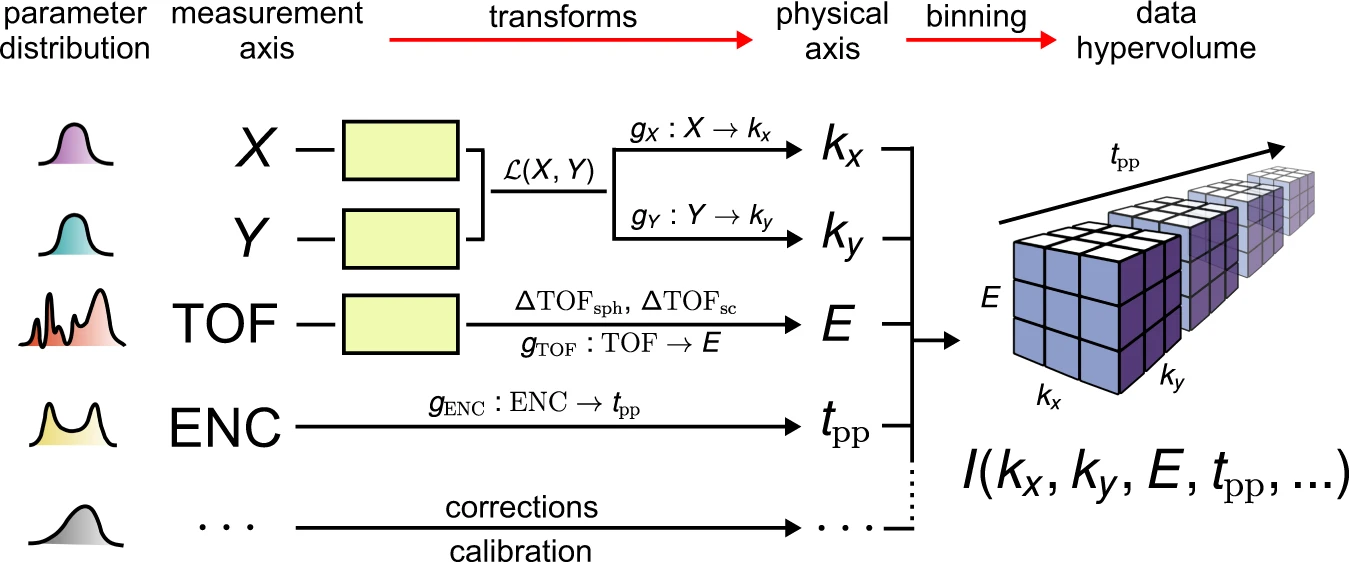
\includegraphics[width=1\linewidth]{images/2024-08-25-22-36-44.png}
    \caption{MPES taken from \cite{xianOpensourceEndtoendWorkflow2020}}
    % \label{fig:enter-label}
\end{figure}

\section{SASE FELs}

\section{HEXTOF Setup at FLASH}
\gls*{DESY} is a national 
\begin{figure}
    \centering
    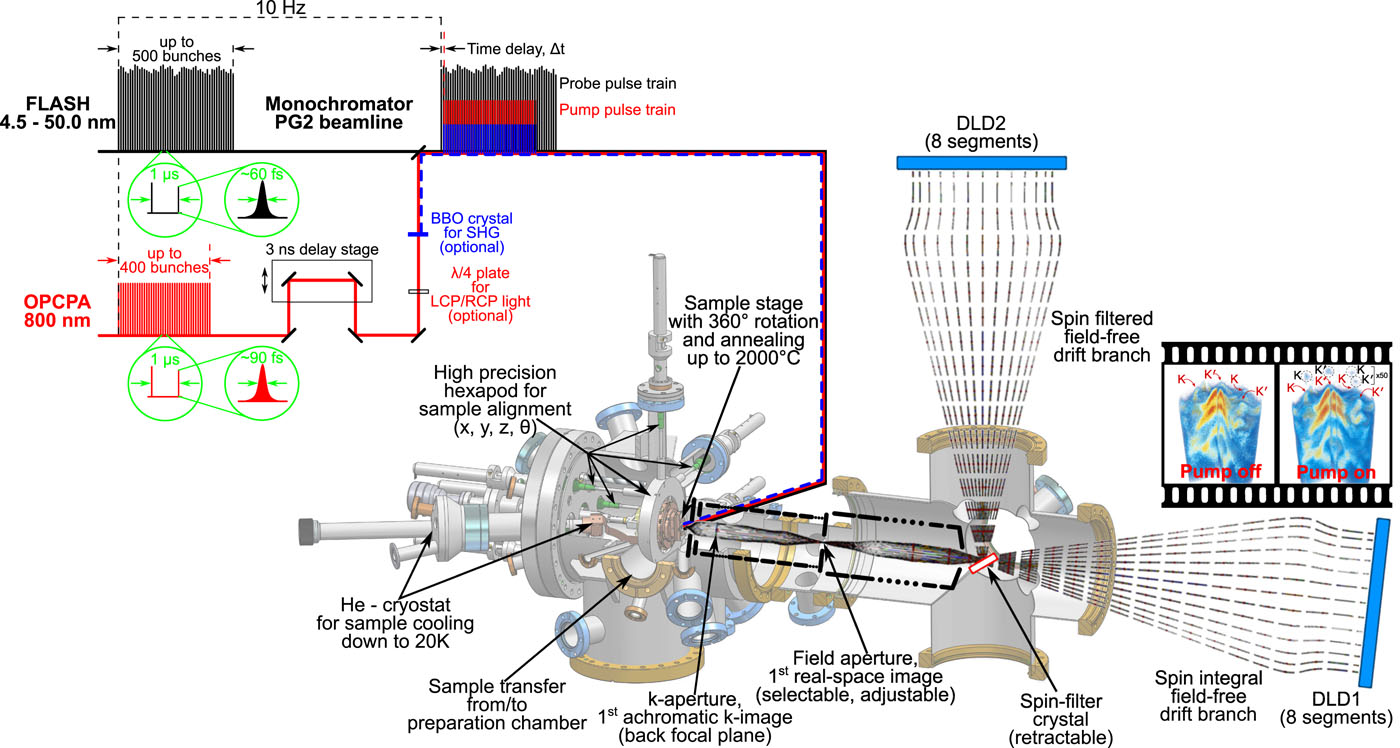
\includegraphics[width=1\linewidth]{images/2024-08-27-10-50-01.png}
    \caption{HEXTOF taken from \cite{kutnyakhovTimeMomentumresolvedPhotoemission2020}}
    % \label{fig:enter-label}
\end{figure}



\chapter{Denoising preliminaries and BM3D}\label{ch:denoising}
Rather than calling it denoising, better word in image reconstruction because
Image Reconstruction:

Purpose: To reconstruct an image from incomplete, noisy, or indirect measurements. This is often used in medical imaging (e.g., MRI, CT scans), computational photography, and computer vision applications. 

Reconstruction involves generating a complete image from partial or indirect data, which can include denoising and deblurring as sub-tasks.

\section{Address reconstruction/denoising schemes}
VST with BM3D: BM3D uses collaborative filtering, which is also used in recommender systems [citation need]
PnP iterative stuff
maybe non local sometime
UNET noise2noise

\section{What is poisson}

\begin{figure}
    \centering
    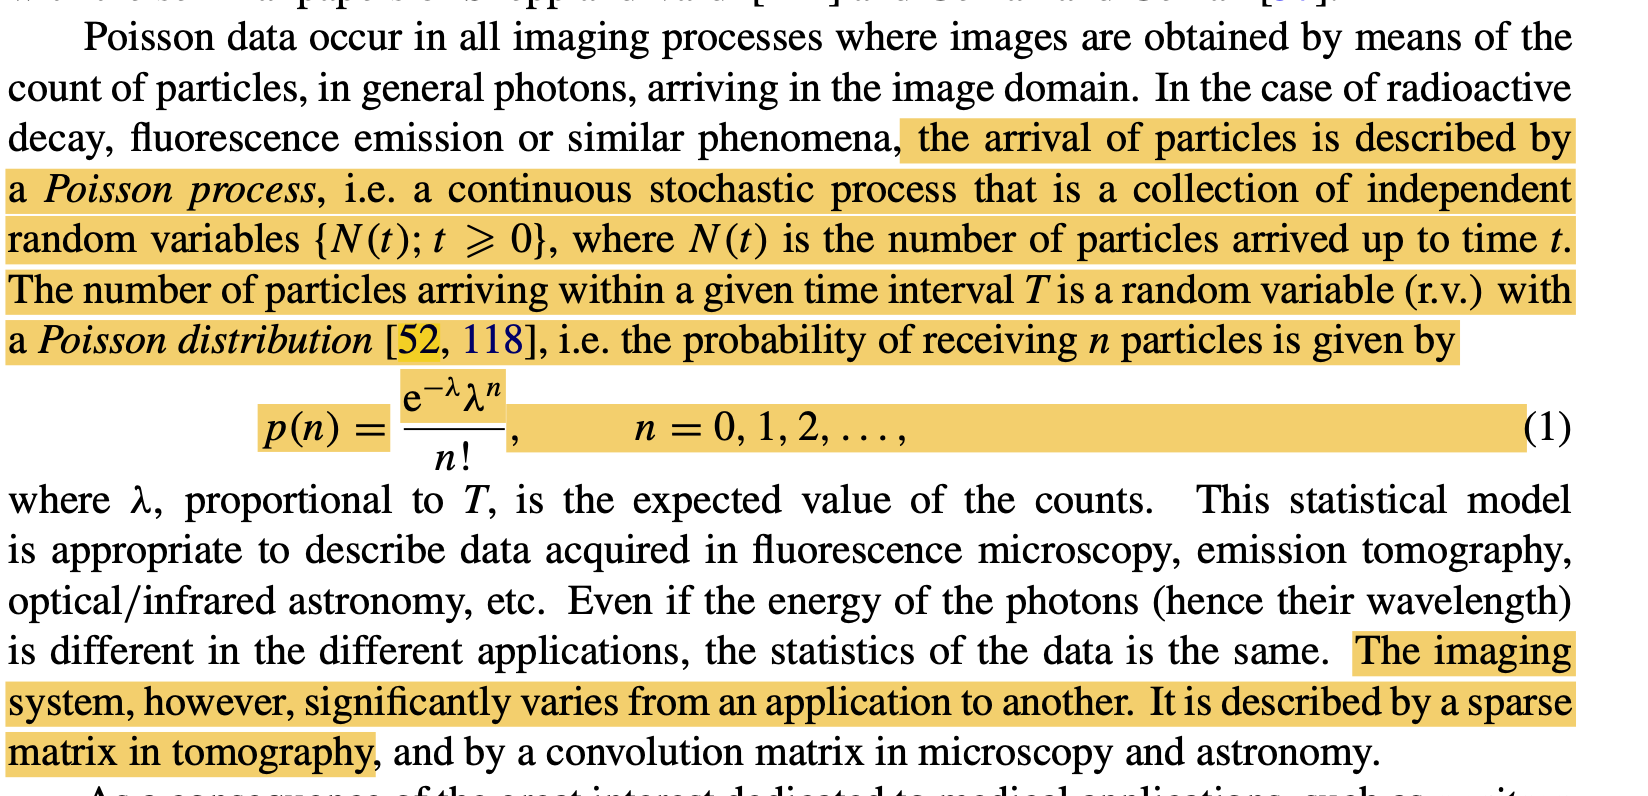
\includegraphics[width=1\linewidth]{images/JD-54-image.png}
    \caption{Enter Caption}
    \label{fig:enter-label}
\end{figure}

Taken from \cite{bertero_image_2009} which cites \cite{feller_introduction_1968}

\section{Comparsion of bm3d }
with and without anscombe on different datasets from flash, lab and fhi
Testing s

\section{Algorithms}

ERM 
Deep learning is just linear sepeartor problem with a non linear function applied to it like RELU
% Rather than calling it denoising, better word in image reconstruction because
Image Reconstruction:

Purpose: To reconstruct an image from incomplete, noisy, or indirect measurements. This is often used in medical imaging (e.g., MRI, CT scans), computational photography, and computer vision applications. 

Reconstruction involves generating a complete image from partial or indirect data, which can include denoising and deblurring as sub-tasks.

\section{Address reconstruction/denoising schemes}
VST with BM3D: BM3D uses collaborative filtering, which is also used in recommender systems [citation need]
PnP iterative stuff
maybe non local sometime
UNET noise2noise

\section{What is poisson}

\begin{figure}
    \centering
    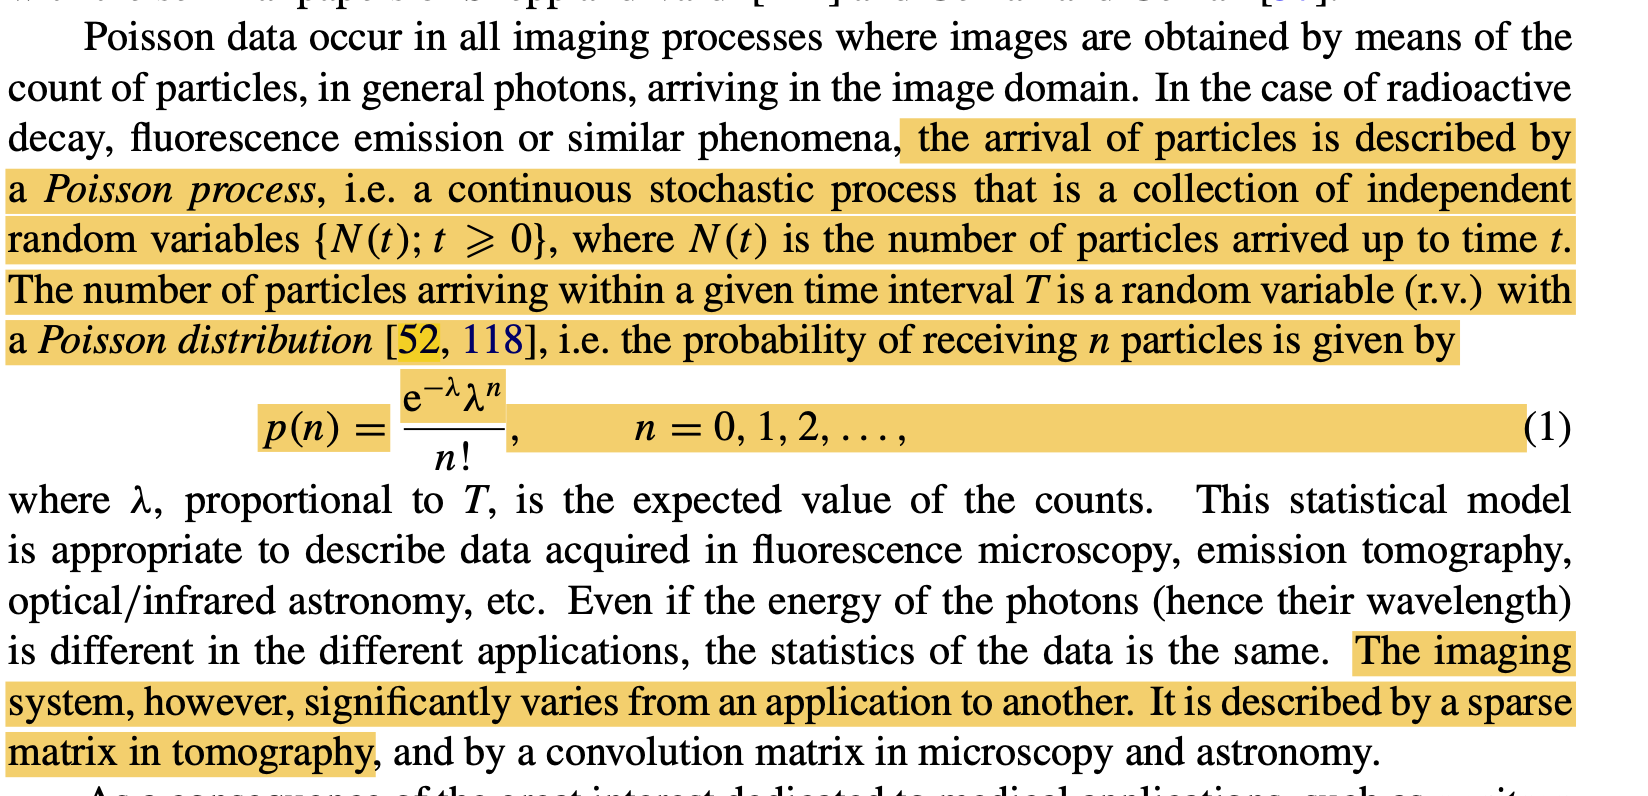
\includegraphics[width=1\linewidth]{images/JD-54-image.png}
    \caption{Enter Caption}
    \label{fig:enter-label}
\end{figure}

Taken from \cite{bertero_image_2009} which cites \cite{feller_introduction_1968}

\section{Comparsion of bm3d }
with and without anscombe on different datasets from flash, lab and fhi
Testing s

\section{Algorithms}

ERM 
Deep learning is just linear sepeartor problem with a non linear function applied to it like RELU

\chapter{Characterizing Photon and Photoelectron Statistics}\label{ch:pes-statistics}
To attempt at reconstructing the latent signal from incomplete observations, it is generally of interest to understand the underlying statistics, as this informs both noise characteristics and the likelihood of different observations. In many imaging and detection systems, especially those involving photons and photoelectron emissions, the observed data is inherently stochastic. Classical and quantum optics provide a comprehensive theoretical foundation to explain photon statistics. For instance, it is well understood that photons from a coherent light source follow a Poisson distribution (an outcome \cref{sec:poisson-noise-model} was based on), often referred to as shot-noise. Whereas, for chaotic (bunched) light, the variance exceeds that compared to their mean, dubbed super-Poissonian. And finally for a squeezed light source, the distribution is sub-Poissonian \cite[Chapter~5]{foxQuantumOpticsIntroduction2006}. The same principle can be extended to photoelectron emission. When photons interact with a material, the resulting photoelectron emission follows the same statistical behavior as the incident photons \cite{mandelFluctuationsPhotonBeams1958,mandelFluctuationsPhotonBeams1959}. 

In this chapter, we begin by formally defining a general model for describing photoelectron event data using a \gls{PPP}, that captures the Poisson-distributed counting statistics for coherent light sources and the \gls{NB} distribution for \gls{SASE} \glspl{FEL}. These model are then tested for counting statistics of photoemitted electrons on data from a pulsed coherent light source and a \gls{SASE} \gls{FEL}.

\section{Modelling Photoelectron Statistics}\label{section:photoelectron-counting-stats}
Let us start by developing an intuition for why photons exhibit stochastic behavior. Photons are the quantized form of electromagnetic light and can be thought of as discrete energy packets. The energy of a photon is given by $E = h\nu$, where $h$ is the Planck constant and $\nu$ is the frequency of the light. Due to the discrete nature of photons, it can be shown that the number of photons in a short time interval $\Delta t$ is not constant. These fluctuations are known as photon shot noise.

For a light source with a constant flux\footnote{Flux is the average number of photons passing through the cross-section of a beam per unit time.} $\phi$ such as a single-mode laser, the average number of photons in a beam segment of length is given by $L$, $\lambda = \phi \frac{L}{c}$, where $c$ is the speed of light. If we subdivide this $L$ into many small intervals  of size $L/N$, where $N$ is large enough so that there is low probability of a photon being in an interval, eventually there will be divisions with no photons, divisions with only single photon, and negligible divisions with multiple photons. For all possible orderings, the probability of finding $n$ subdivisions with a single photon and $(N-n)$ with no photons can be modeled by the Binomial distribution as follows, with $p=\frac{\lambda}{N}$ being the probability of a photon being in a segment:

\begin{equation}
    P(n) = \binom{N}{n} p^n (1 - p)^{N - n}
\end{equation}

Using the Poisson Limit Theorem \cite{fellerIntroductionProbabilityTheory1991a}, it can be shown that as $N \to \infty$, and the probability $p \to 0$ such that $Np = \lambda$ remains constant, there is a convergence in distribution to the Poisson distribution (\cref{note:poisson-distribution}). Hence, the Poisson distribution is a suitable model for counting statistics of photons from a coherent light source.

\subsection{Photoelectron Counting}
\citeauthor{mandelFluctuationsPhotonBeams1958} \cite{mandelFluctuationsPhotonBeams1958,mandelFluctuationsPhotonBeams1959} and others have shown that the transition probability of an electron from its ground state to an unbounded state at the surface of a photodetector is directly proportional to both the duration of the time interval $\Delta t$ and the instantaneous light intensity $I(t)$. This suggests that the rate density of photoelectrons is proportional to the light intensity $\lambda(t) \propto \int_{A} I(t)$, where $A$ is the detector area.

The aforementioned can be mathematically formalized through one-dimensional stochastic process known as a \gls{PP}\footnote{For a more generalized description of \gls{PP}, the reader is referred to \cite{chiuStochasticGeometryIts2013}.}. A \gls{PP} is used to model occurrences of stochastic events that happen in some space. If we look at the time domain, the \gls{PP} allows us to the model the occurrence of events in time. The process generates a series of time points $\{t_1, t_2, \dots, t_n\}$ where the events occur, within a time interval $[0, T]$.

A \gls{PP} often used to model events is the \glsxtrfull{PPP}, describable by the rate density function $\Lambda(t)$ (also known as the intensity function). The key property of such a process is that the events are statistically independent:

\begin{equation}
    \Lambda(t_1, t_2, \dots, t_n) = \prod_{i=1}^{n} \Lambda(t_i)
\end{equation}

If the rate density function is constant, $\Lambda(t) = \Lambda$, the process is known as a homogeneous (or stationary) \gls{PPP}, such as the case with a coherent laser light source \cite{salehPhotoelectronStatistics1978}. If the rate function is time-dependent and deterministic $\Lambda(t)$, it is known as the inhomogeneous \gls{PPP}. Such a situation could occur when the intensity of light is modulated, as is the case with a pulsed laser source. In a situation such as where the $\Lambda(t)$ itself is a stochastic variable, the process is known as the doubly stochastic \gls{PPP}, or Cox process. 

% Such is the case if the light source is a \gls{SASE} \gls{FEL}, where the intensity of light fluctuates stochastically (see \cref{section:light-sources} for why this happens). Due to this process, the photoelectron counting statistics in this case also deviate from the Poisson distribution, as we shall see later.

Integrating light intensity $I(t)$ over the time interval $\Delta t$ can be treated as a random variable with probability density $P(W)$, with $W$ as:
\begin{equation}
    W = \int_{\Delta t}^{t+\Delta t} I(t') dt
\end{equation}

The probability of detecting $n$ photoelectrons in that time interval is then given by the Poisson transform relation \cite{mehtaVIIITheoryPhotoelectron1970} (a realization of the doubly stochastic \gls{PPP}):
\begin{equation}\label{eq:mandel-photo-electron}
    P(n, t, \Delta t) = \int_{0}^{\infty} \frac{\alpha W^n}{n!} e^{-\alpha W} P(W) \, dW
\end{equation}

With a constant intensity light source, $W$ becomes deterministic and \cref{eq:mandel-photo-electron} simplifies to a Poisson distribution:
\begin{equation}
    P(n, t, \Delta t) = \frac{W^n e^{-W}}{n!} 
\end{equation}

Due to the \gls{SASE} process of an \gls{FEL} light, discussed briefly in \cref{section:light-sources}, the light intensity fluctuates stochastically. This leads to the photoelectron counting statistics being over dispersed and deviating from the Poisson distribution. \citeauthor{saldinStatisticalPropertiesRadiation1998} have shown in \cite{saldinStatisticalPropertiesRadiation1998} that the photoelectron counting statistics from a \gls{SASE} \gls{FEL} light source can be modeled by a \gls{NB} distribution (\gls{PMF} and other details defined in \cref{note:negative-binomial-distribution}), a realization of the Cox process. And due to the light and photoelectron statistics relation, the photoelectron counting statistics also follow the same distribution.

The important thing to note here is that above discussion is about the statistics of photoelectrons from photon detection. Whereas, our experiment is of \gls{PES}, where we are then interested in the (detected) emitted electrons (electron count distributions).

\section{Testing of Counting Statistics}
There are two simple ways to test a \gls{PPP}\footnote{Specialized tests do exist to directly test for a homogeneous \gls{PP}, hypothesizing complete spatial randomness. Ripley's K-function can be used as a goodness of fit test \cite[Section~2.6.4]{chiuStochasticGeometryIts2013}. However, these do not test for the doubly stochastic \gls{PPP}.}. \textit{The interval statistics}, where the time intervals between events $\Delta t$ should follow an exponential distribution for a \gls{PPP}. The other is \textit{counting statistics}, where the number of events ($\gls{ncounts}$) within a fixed time interval $\Delta t$ should follow a distribution based on \cref{{eq:mandel-photo-electron}}.

We consider the latter case, for two reasons. First, from the discussion above, we have well-established hypotheses between the expected distributions for different light sources. Second, the timing information from the light source is coarser than the electron detection time. While the \gls{DLD} detector measures the \gls{TOF} of each electron, allowing us to get individual timing, the detector's dead-time could influence the time-interval statistics. Therefore, we analyze the \textit{counting statistics}.

\begin{figure}
    \centering
    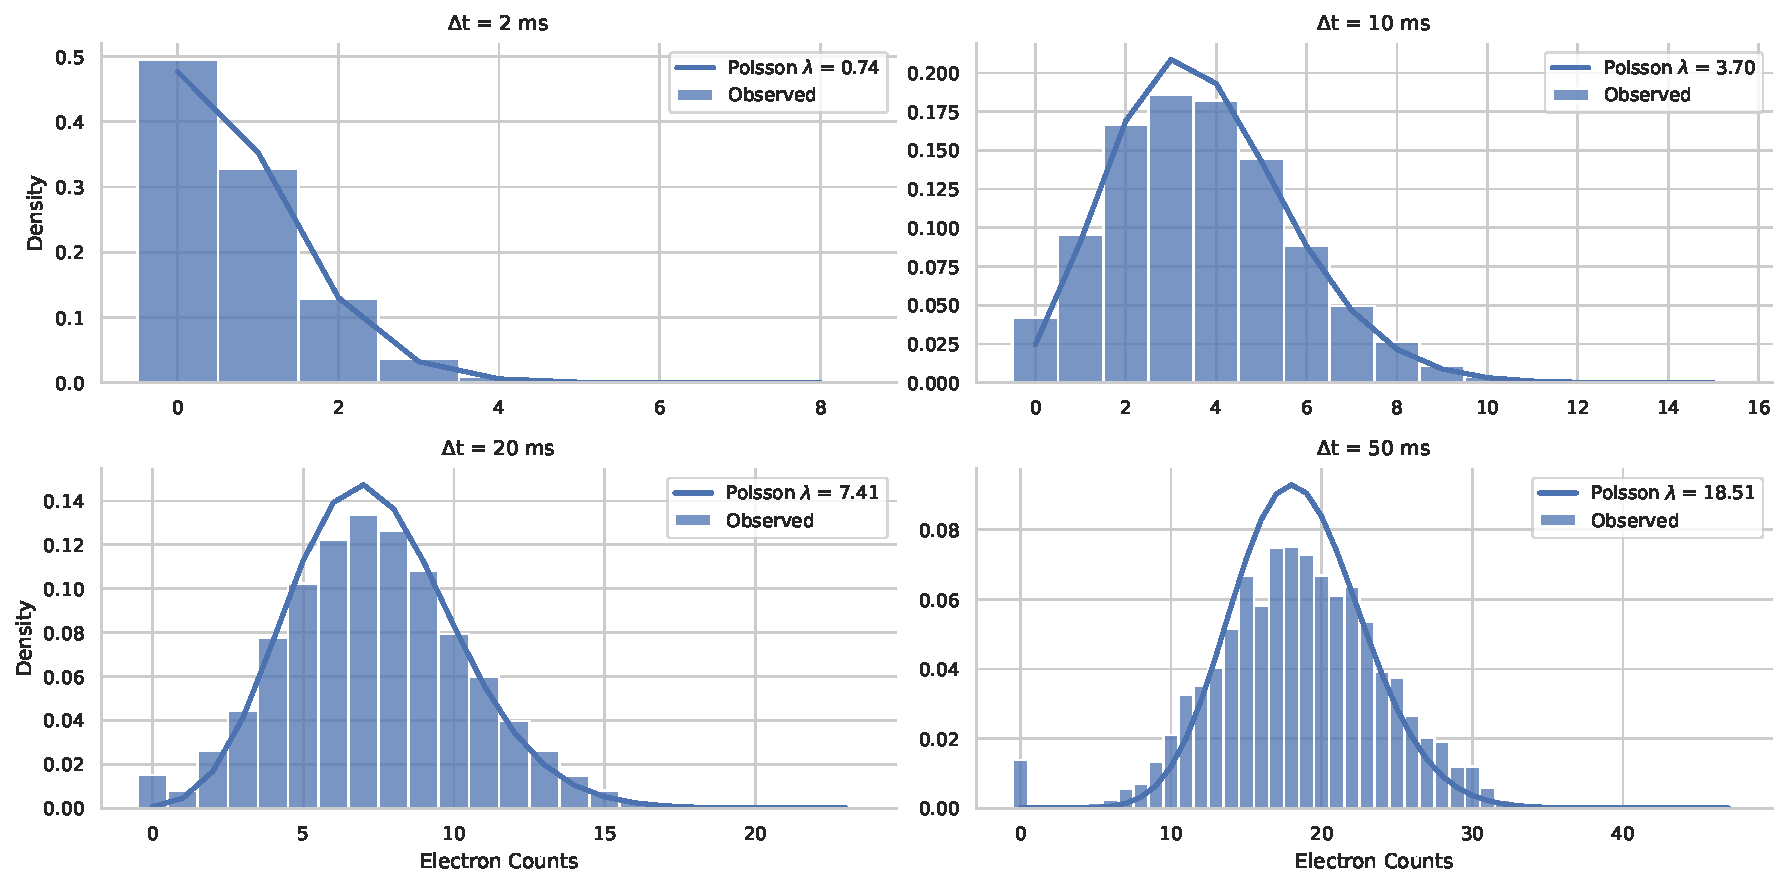
\includegraphics[width=1\linewidth]{images/hist_counts_facetgrid_1_wse2.pdf}
    \caption{Distribution of photoelectron counts at time intervals $\Delta t =$ \qtylist{2;10;20;50}{ms} for a selected volumetric subset of the full \gls{WSe2} dataset. Poisson statistics are observed at smaller time intervals, but as the time window increases ($\Delta t = \qty{50}{ms}$), the data starts to deviate from the Poisson distribution, as spatial correlations become apparent. The total counts in this selected region are $\gls{ncounts}=\num{4.7e4}$ with total observation time $T=\qty{126}{s}$.}
    \label{fig:wse2-stats}
\end{figure}

We test the counting statistics observed for \gls{PES} at two different light sources: a pulsed \gls{HHG} laser (\gls{WSe2} dataset), and a \gls{SASE} \gls{FEL} light source (\gls{GrIr} dataset). Based on theoretical considerations, we hypothesize that the counting statistics of the photoelectrons from the laser source would align a Poisson distribution, and from the \gls{SASE} \gls{FEL} source, with a \gls{NB} distribution. 
% The hypothesized counting statistics are tested using the Poisson dispersion test, and if that is rejected, using the Chi-Square test (for details regarding this, refer to \cref{section:chi-test}).

While the \gls{PPP} should exhibit the same counting statistics for any time window $\Delta t$, practical challenges such as the long-term measurement drifts in intensity, can make that hard to realize. To account for this, we will analyze several time intervals to determine if the statistics remain valid based on the light source used. Given that the goal of \gls{MPES} is to map band structures whose feature sizes are generally much larger than a single voxel, the data inherently exhibits spatial correlations\footnote{Spatial here means in the image space, which also includes the time delay axis.}. An ideal experimental setup to measure counting statistics would instead minimize spatial correlations and allow for long acquisition times to obtain reliable statistical estimates across different time windows.

In our analysis, we consider the detector-defined 3D subsets of data, which are often sparsely populated. While the most precise assessment of counting statistics would involve analyzing a single voxel, the sparsity of the data necessitates examining small subsets of the 3D volume instead. We select sufficiently small $\Delta t$ to ensure that spatial correlations have minimal impact on the observed statistics, and also look at the cases where it is high.

\subsection{HHG Light Source}
Let us look at the dataset using \gls{HHG} laser first: \gls{WSe2}. \cref{fig:wse2-stats} shows the count distribution at $\Delta t =$ \qtylist{2;10;20;50}{ms}, with an observation time $T=\qty{126}{s}$, and one specific volumetric subset. The count distributions for smaller time intervals ($\Delta t = \qtylist{2;10;20}{ms}$) follow Poisson statistics, as expected from an uncorrelated photoemission process where spatial and temporal fluctuations are minimal. However, for longer time intervals ($\Delta t = \qty{50}{ms}$), the distribution starts to deviate from the Poisson distribution. This deviation suggests that spatial correlations, due to the material properties of the sample, become significant enough to impact the distribution. While the impact of pulse light source should be minimal since the time intervals we look at are much longer than the pulse durations, the intensity drifts could also cause the deviation. \cref{fig:wse2-stats-2} shows count statistics from a different volumetric subset, forming the same conclusions.

From the above, we can conclude that the photoemitted electrons statistics are a realization of a \gls{PPP}. \citeauthor{heimerlMultiphotonElectronEmission2024} \cite{heimerlMultiphotonElectronEmission2024} have also recently showed that the emitted electrons show a Poisson distribution with a (coherent) pulsed laser light source.

To determine the homogeneity of the process, if we look at $\Delta t = \qty{50}{ms}$ in both \cref{fig:wse2-stats} and \cref{fig:wse2-stats-2}, the zero counts start forming a bimodal characteristic. This could be attributed to the pulse structure of the laser light source, where the absence of photons between pulses leads to a high occurrence of zero counts. Hence, due to this inhomogeneity in intensity, the  statistics might be better modeled with an inhomogeneous \gls{PPP}. For a pulsed light source with pulse interval $\tau_{\text{pulse}}$, the counting statistics should still be Poisson for $\Delta t >> \tau_{\text{pulse}}$, and otherwise due to regular spacing when no events occur, it is better modeled by an inhomogeneous \gls{PPP}.

% Applying the Poisson dispersion test at a significance level of $\alpha=0.05$ for \num{1000} samples at each $\Delta t$ of \qtylist{2;10;20;50}{ms}, we report $p$-values of \numlist{0.88;0.87;0.10;0.00}, respectively. The test fails to reject the null hypothesis of Poisson distribution for $\Delta t = \qtylist{2;10;20}{ms}$, but rejects it for $\Delta t = \qty{50}{ms}$.

It must be noted that for \gls{HHG} sources, \citeauthor{gorlachQuantumopticalNatureHigh2020} \cite{gorlachQuantumopticalNatureHigh2020} have shown that the highly non-linear \gls{HHG} process can significantly affect the photon statistics. They have shown that depending on the generated harmonic, the photon statistics vary, with some harmonics able to exhibit squeezed light properties, and others over-dispersion. The seventh harmonic (\qty{21.7}{eV}) up-converted to \gls{XUV} via \gls{HHG} was used for the \gls{PES} of \gls{WSe2} \cite{maklarQuantitativeComparisonTimeflight2020}. Hence, in view of the above-mentioned work, further studies are required to understand the photon and the corresponding photoemitted statistics.

\begin{figure}
    \centering
    \begin{subfigure}[t]{0.49\linewidth}
        \centering
        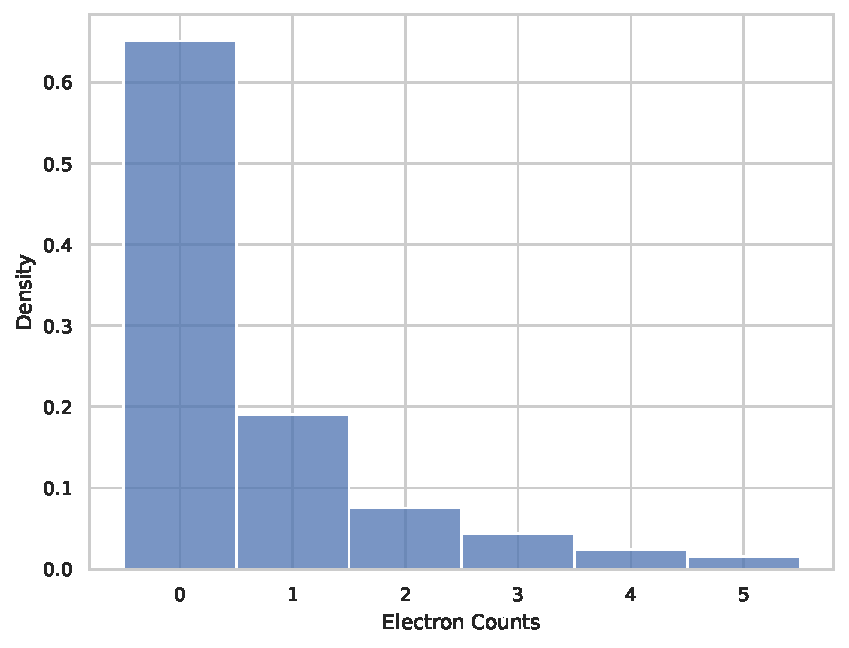
\includegraphics[width=\linewidth]{images/hist_counts_1_layer.pdf}
        \caption{Single layer of the \gls{DLD}.}
        \label{fig:grir-stats-1-layer}
    \end{subfigure}
    \hfill
    \begin{subfigure}[t]{0.49\linewidth}
        \centering
        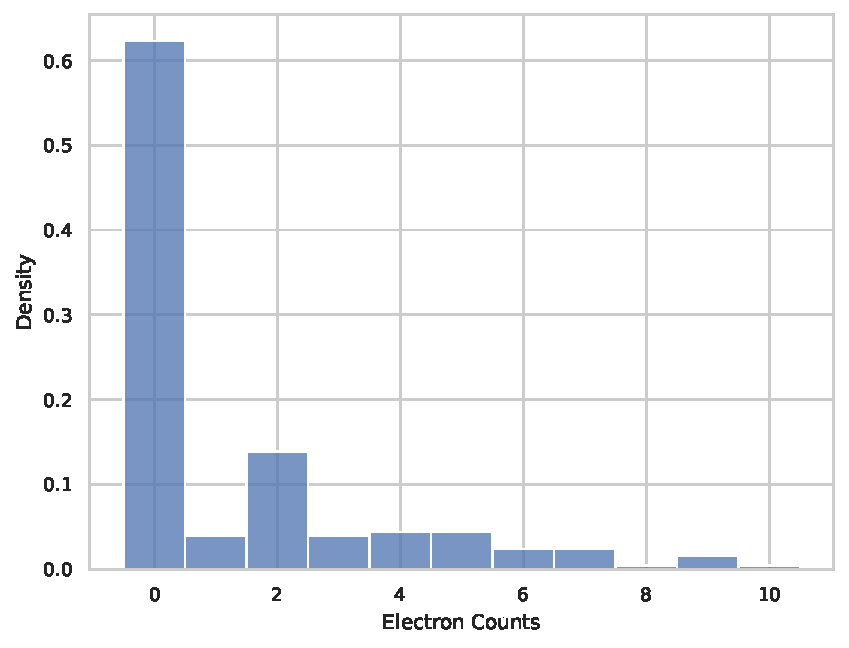
\includegraphics[width=\linewidth]{images/hist_counts_2_layer.pdf}
        \caption{Both layers of the \gls{DLD}.}
        \label{fig:grir-stats-2-layer}
    \end{subfigure}
    \caption{Counting statistics comparison for single layer or both layers of the \gls{DLD}. It is clear that the incorrect counting influences the statistics significantally.}
    \label{fig:grir-stats-dld-comparison}
\end{figure}

\subsection{SASE FEL Light Source}
Analyzing this data requires a few additional considerations. In \cref{section:dld}, we already saw that the \num{8}S \gls{DLD} shows repeated counts for a single electron, due to the segmented structure. From preliminary analysis of counting statistics shown in \cref{fig:grir-stats-dld-comparison}, it can be seen that this has a significant impact on the counting statistics, where the \num{2}-event occurrence is unnaturally high compared to the others (\cref{fig:grir-stats-2-layer}). Therefore, this analysis will only consider a single layer (from the 2-layered delay-line structure), and ideally a volumetric subset from a single segment\footnote{Due to the overlap between segments.}.



\begin{figure}
    \centering
    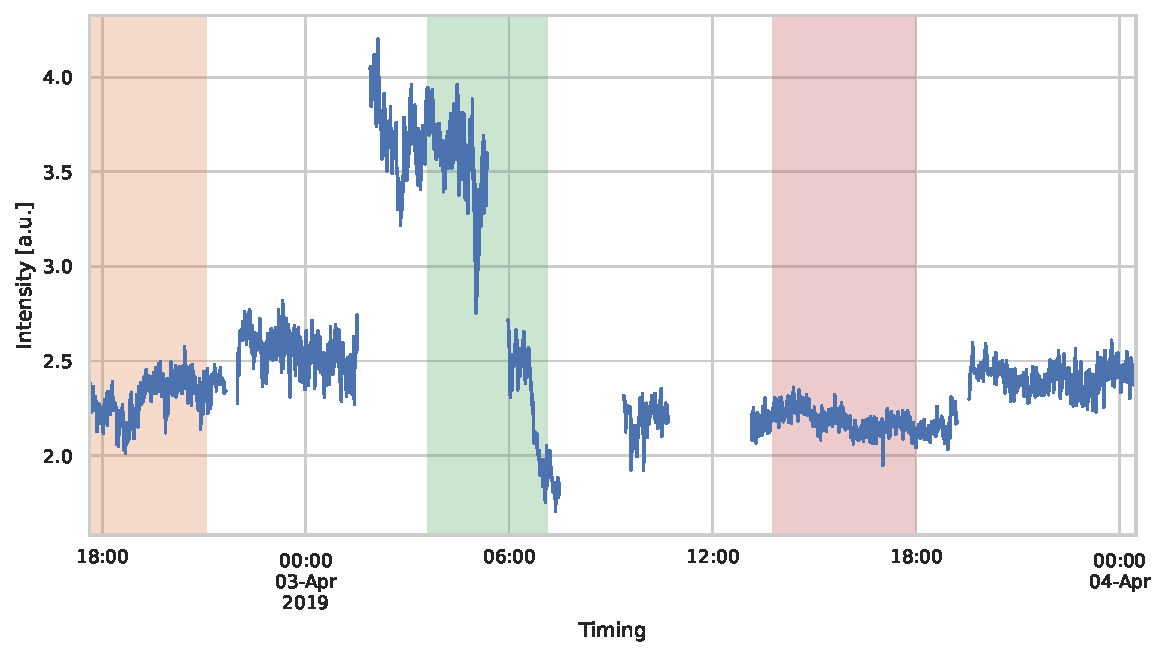
\includegraphics[width=0.8\linewidth]{images/gmd_grir.pdf}
    \caption{Beam intensity measurements, using the \gls{GMD} over the time period $T=\qty{30}{hour}$, with data window-averaged at \qty{1}{min} intervals. The fluctuations in intensity can be observed, an intrinsic property of the \gls{SASE} process. Other notable observations are the long-term drifts in intensity, and the beam interruptions (no recorded values). The orange, green and red spans indicate the time periods used for other analyses.}
    \label{fig:gmd-intensity}
\end{figure}


\begin{figure}
    \centering
    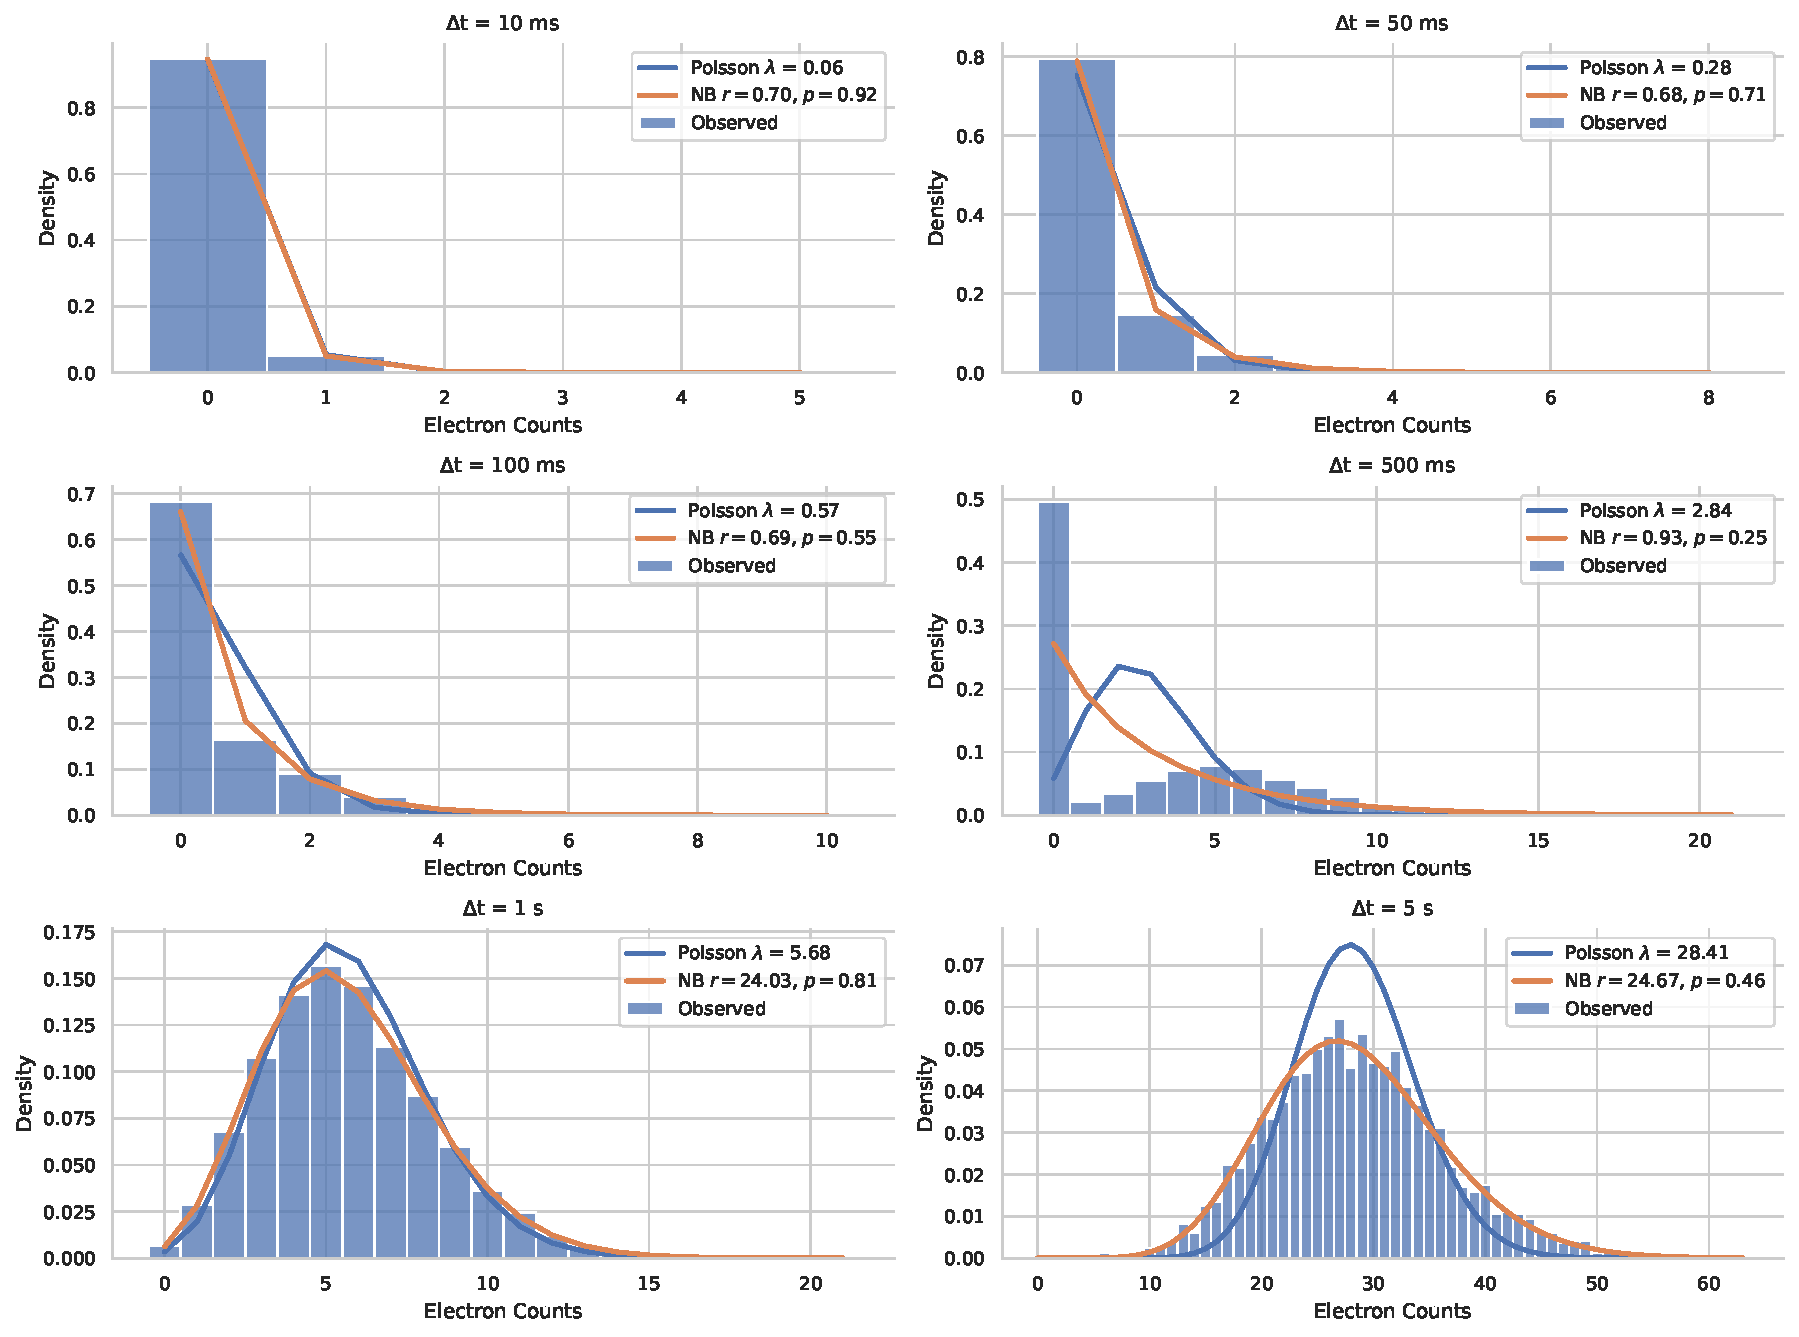
\includegraphics[width=1\linewidth]{images/hist_counts_facetgrid_1_grir.pdf}
    \caption{Distribution of photoelectron counts at time intervals $\Delta t =$ \qtylist{10;50;100;500;1000;5000}{ms} for a selected volumetric subset of the full \gls{GrIr} dataset. At shorter time intervals $\Delta t \leq \qty{50}{ms}$, Poisson statistics provide a good fit, reflecting the limiting case where the \gls{NB} distribution approximates Poisson behavior. However, as the time interval increases, the distribution shows significant over-dispersion, with a pronounced right-skew characteristic of the \gls{NB} distribution. Notably, at $\Delta t = \qty{500}{ms}$, the pulsed structure of the \gls{FEL} becomes apparent, resulting in a high occurrence of zero counts. The total counts for this selected region are \gls{ncounts} = \num{8e5}, with a total observation time of approximately $T = \qty{4}{h}$ (refer to the orange region in \cref{fig:gmd-intensity})}.
    \label{fig:grir-stats-1}
\end{figure}


The second consideration is the long-term intensity drifts in the \gls{FEL} light source. \cref{fig:gmd-intensity} shows the beam intensity measurements\footnote{Measured using \gls{GMD}, see \gls{gmd}} over the time period $T=\qty{30}{hour}$, with data window-averaged at \qty{1}{min} intervals. The long-term drifts in intensity, and the beam interruptions due to accelerator operation can be observed. For analysis, we look at the data from the orange, green, and red spans. With no beam interruptions in the orange and red span, the expectation is that it follows the \gls{NB} distribution. Whereas, the counting statistics would differ in the green span due to the beam interruptions.


We continue looking at the \gls{GrIr} dataset from previous chapters. We look at a broad range of time intervals, as the count rate is much lower compared to the \gls{HHG} source. The pulse structure of the \gls{FEL} is more complex, as illustrated in \cref{fig:hex-tof}. The macrobunches (see \gls{train}) arrive at a repetition rate of \qty{10}{Hz}, meaning a new train of \glspl{pulse} arrives every \qty{100}{ms}.


\cref{fig:grir-stats-1} show photoelectron count distributions for varying time windows ($\Delta t =$ \qtylist{10;50;100;500;1000;5000}{ms}) within the orange span of \cref{fig:gmd-intensity}, with a total observation time of $T=\qty{4}{h}$. At $\Delta t = \qty{10}{ms}$, the Poisson and \gls{NB} fit approximately match. Increasing the time interval starts to show better fit with \gls{NB} than Poisson, with a pronounced right-skew characteristic. Notably, $\Delta t = \qty{500}{ms}$ has a high occurrence of zero counts, which could highlight the pulsed structure of the \gls{FEL}, having regions within each train that have no photons. At $\Delta t = \qty{5000}{ms}$, the deviation from Poisson is apparent, with a significant over-dispersion. \cref{fig:grir-stats-3} shows the same analysis for the red span, with similar conclusions.

\cref{fig:grir-stats-2} shows the interesting regime (green span). The frequency of zero counts clearly deviates from any hypothesis, and is only explainable by the beam interruption, and significant intensity difference. The intensity variation effect is clearly visible at $\Delta t = \qty{5000}{ms}$, where asides from the zero counts, the distribution is bimodal, highlight two distinct count rates.

In summary, the analysis of photoelectron counting statistics from the \gls{FEL} light source highlights the complexity of the data influenced by the detector’s structure, the \gls{SASE} and long-term intensity fluctuations. The \gls{NB} distribution is shown to be a more suitable model for such case. However, for the aim of reconstructing the latent distribution from incomplete observations, the spatial correlations induced by the material under study, and the detector structure should also be considered in the estimation process.


\begin{figure}
    \centering
    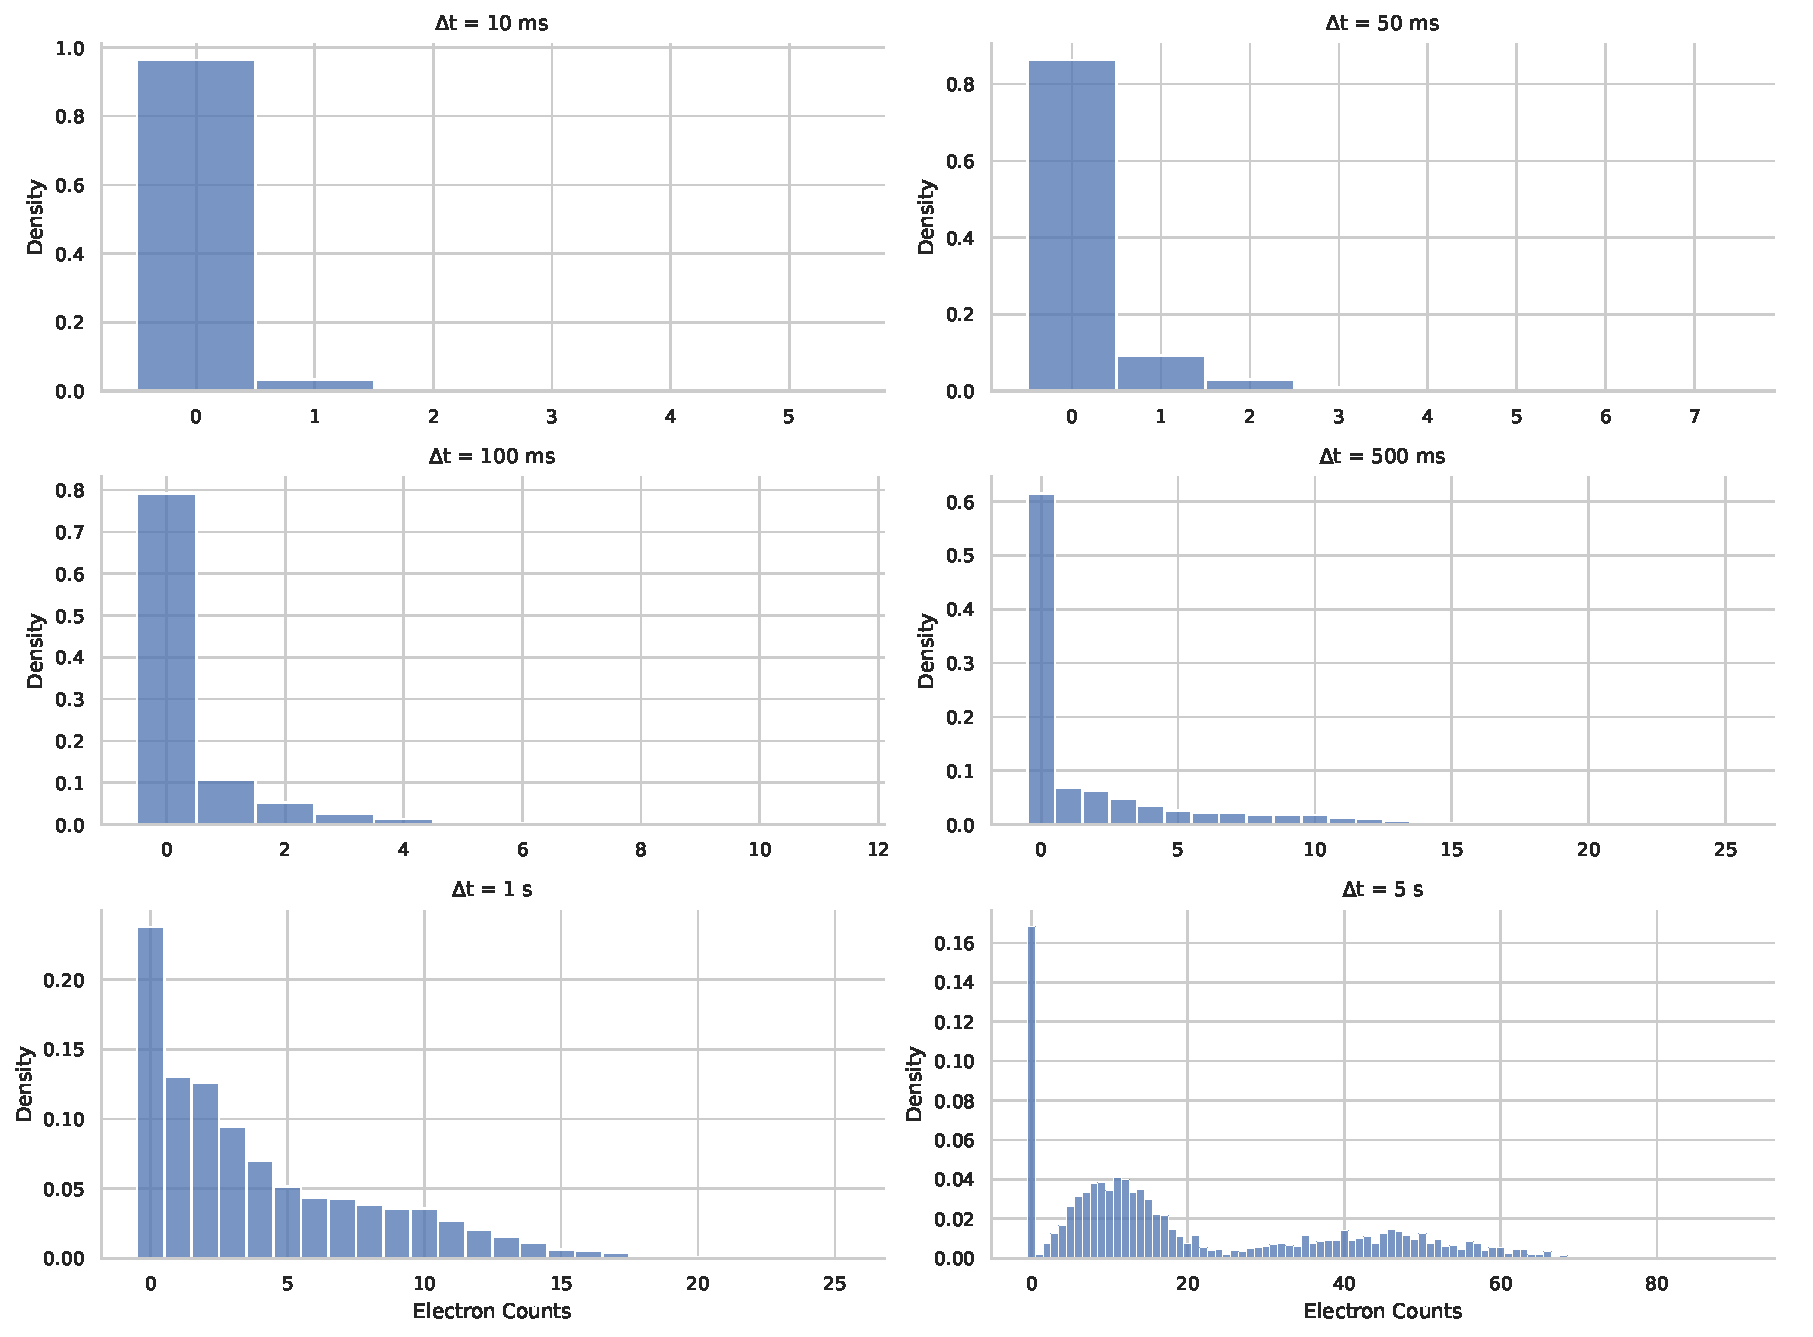
\includegraphics[width=1\linewidth]{images/hist_counts_facetgrid_2_grir.pdf}
    \caption{Distribution of photoelectron counts at time intervals $\Delta t =$ \qtylist{10;50;100;500;1000;5000}{ms} for a selected volumetric subset of the full \gls{GrIr} dataset. The total counts in this selected region are $\gls{ncounts}=\num{5e5}$ with total observation time $T\approx\qty{3.5}{h}$  (See green region in \cref{fig:gmd-intensity}). Neither Poisson nor \gls{NB} statistics provide a good fit for any of the time intervals. The frequency of zero counts is significantly higher, and the distribution is bimodal at $\Delta t = \qty{5000}{ms}$, indicating a significant intensity difference.}
    \label{fig:grir-stats-2}
\end{figure}

% \begin{figure}[t]
%     \centering
%     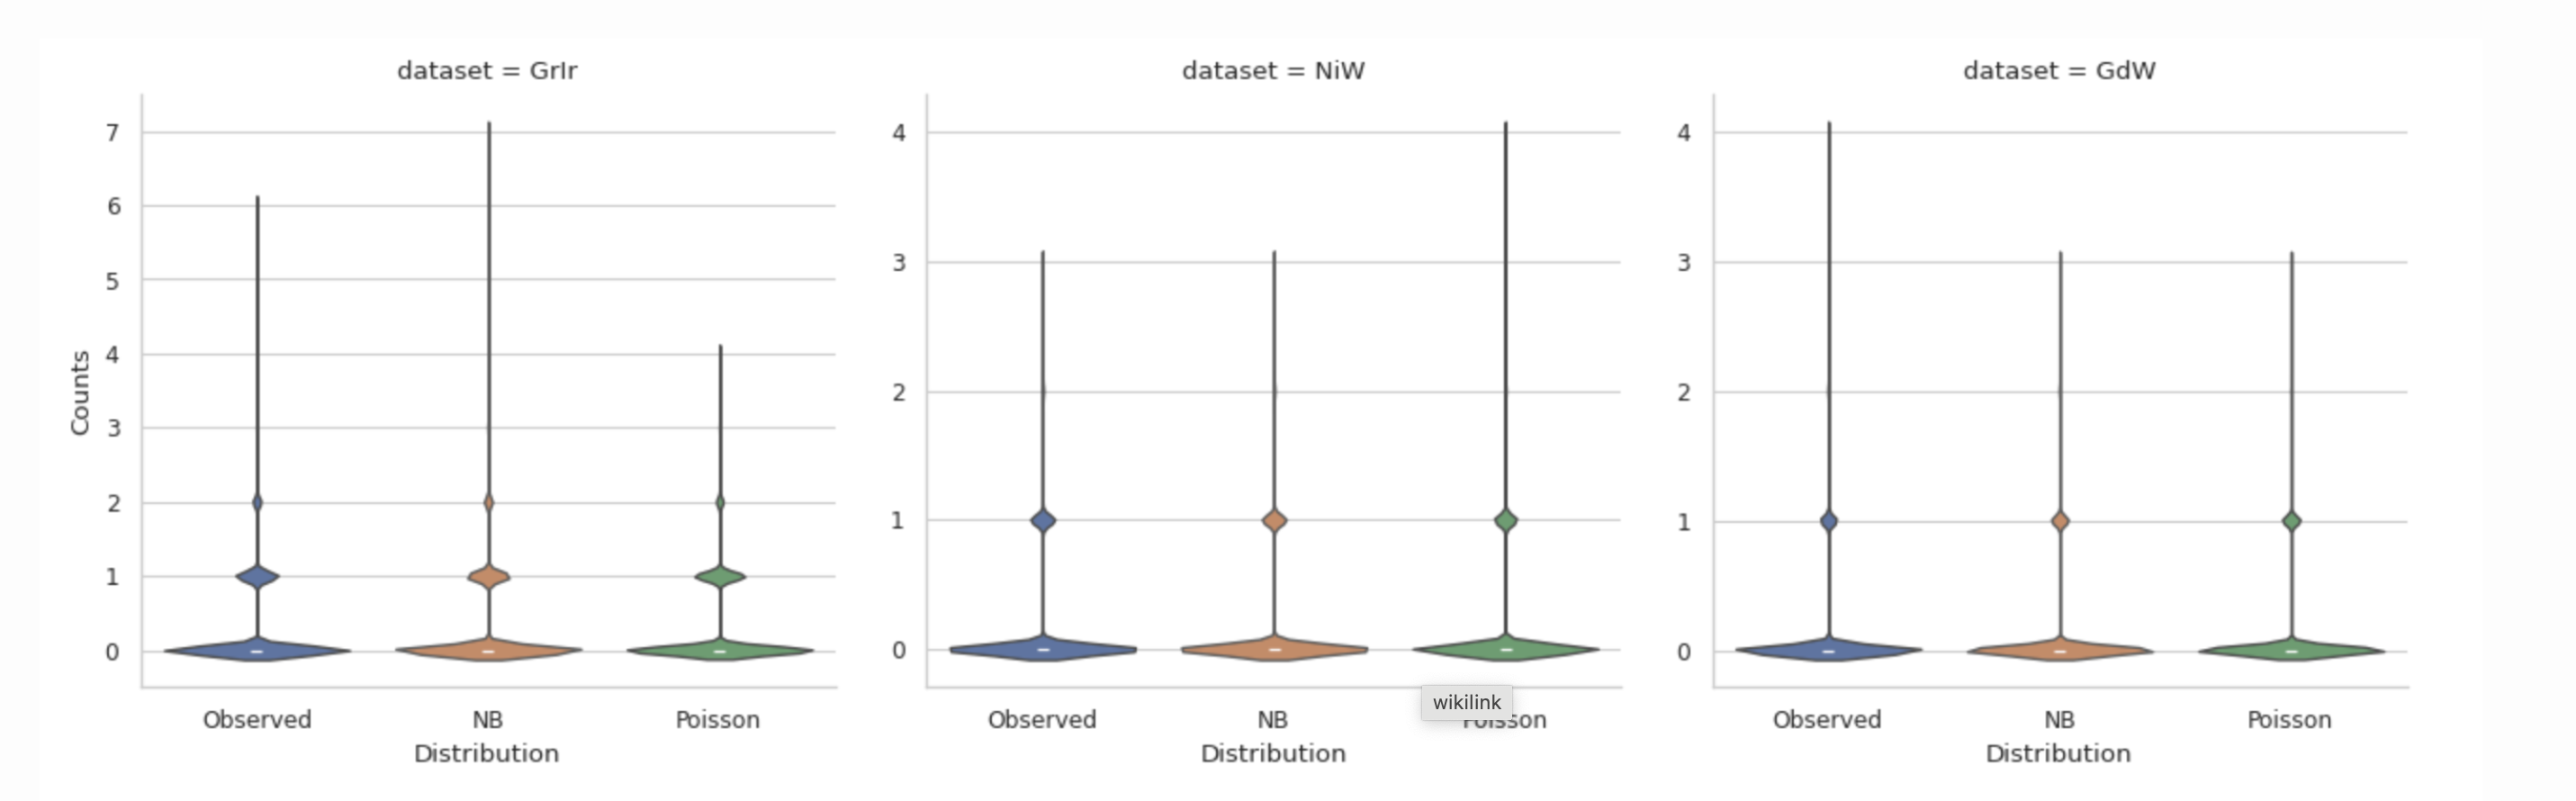
\includegraphics[width=1\linewidth]{images/violin_plots_per_pulse.png}
%     \caption{Enter Caption}
% \end{figure}

% \begin{figure}[htbp]
%     \centering
%     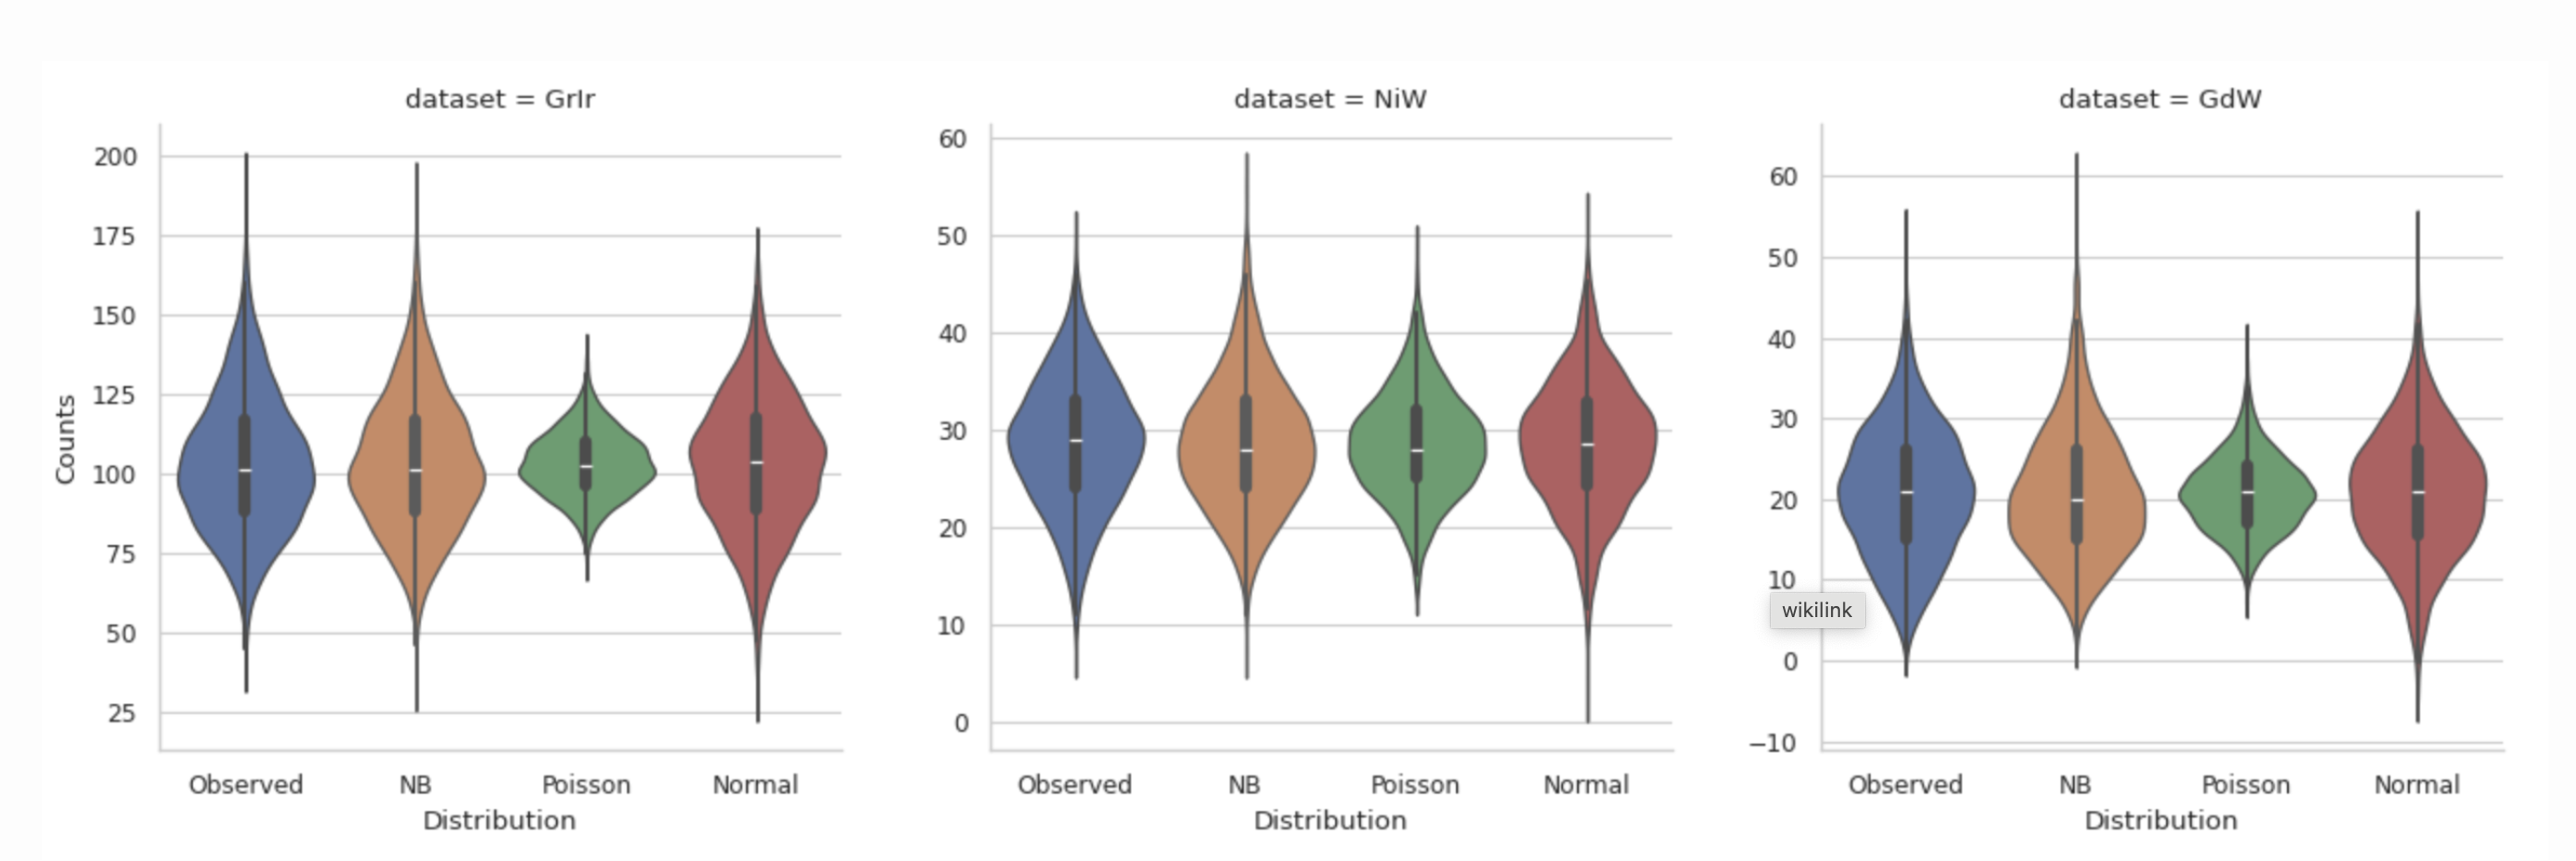
\includegraphics[width=1\linewidth]{images/violinplots_per_train.png}
%     \caption{ss}
%     \label{s}   
% \end{figure}

% \subsection{Analysis of Photoelectron Counting Statistics}

\chapter{Learning from Noise}\label{ch:deep_learning}
\todo[disable]{I would put more references into this Chpater.}
In Chapter~\ref{ch:pes-statistics}, we saw that the photoemission statistics are influenced by the characteristics of the light source, that exhibit well-defined statistical properties. Understanding these specific characteristics can be helpful in designing tailored, model-based denoisers. For Poisson noise, we employed the Anscombe transform combined with \gls{BM3D} (\cref{sec:poisson-noise-model}). While the Anscombe transform is capable of stabilizing Poisson-distributed noise into approximately Gaussian noise for moderate to high counts, it is less effective for very low counts ($<3$) and the approximation breaks down as discussed previously in \cref{sec:poisson-noise-model}. Whereas, a \gls{VST} tailored for \gls{NB} statistics in conjunction with \gls{BM3D} could be more effective to reduce noise.

Model-based approaches such as these can be powerful but they assume that the noise characteristics are accurately known and that the underlying signal conforms to the priors encoded. However, \gls{FEL}-based photoemission experiments involve complex and heterogeneous noise sources. Factors such as long-term fluctuations in \gls{FEL} intensity (\cref{section:fel-stats}), advanced detector designs (\cref{section:8s-dld}) and environmental variations can lead to deviations from idealized models like Poisson or \gls{NB} noise prior. Adapting model-based methods to account for these complexities requires significant effort and may still fall short when dealing with unknown or dynamically changing noise patterns.

Unlike model-based methods, which depend on predefined assumptions about the noise and other image priors, deep learning, a subset of machine learning, \todo[disable]{``machine and deep learning methods'' sounds like machine learning and deep learning are different things, but the latter is just a special case of the former} can learn these relationships directly from data. This data-driven approach allows deep \todo[disable]{Now there is no mention of machine learning anymore. Perhaps the easiest would be to simply drop the term machine learning above and only talk about deep learning.} learning models to handle diverse and complex noise distributions, including those that are non-standard, multi-modal, or vary across a dataset. Furthermore, \gls{CNN}-based architectures excel at extracting non-linear and hierarchical features from \todo[disable]{It's not clear what this ``such'' is referring to here. In this paragraph you didn't specify data sets. I assume you mean data drawn from complex noise distributions, but you don't explicitly say that.} high-dimensional data structures such as images extracted from \gls{MPES} datasets. This allows to take advantage of the spatial and temporal correlations across multiple dimensions more effectively than many traditional approaches.

Machine learning can be broadly categorized in two categories: the \textit{supervised} and the \textit{unsupervised} setting. In supervised learning, the mapping (\textit{model}) is learned by exposure to labeled data (input-target pairs).\todo{self-supervised learning} \todo[disable]{This is a somewhat implicit, somewhat complicated way to describe this. I think it would be easier if you first state the task, i.e., to learn a mapping, and you do that based on given input/output pairs, i.e. the training data.}. The exposure to such data, \textit{training}, enables the model to establish a relationship between the inputs and the corresponding target. The model’s expertise can then be used to map (predict) new inputs to the desired targets. In the context of image restoration, the model can gain expertise from pairs of corrupted (input) and clean images (target), and then use this expertise to restore other corrupted images.

Conversely, in the unsupervised setting, the model is exposed to the data without any labeled information, and the model is supposed to learn the underlying structure of the data. In context of image restoration, that would imply only giving the model the corrupted images, and expecting to map to the desired target--the clean image \cite{ulyanovDeepImagePrior2020,krullNoise2VoidLearningDenoising2018}\todo[disable]{Do you have specific unsupervised deep learning approaches for image restoration in mind? It's quite hard to imagine how this is supposed to be done in an unsupervised manner from this description.}.

In this chapter, the foundations of machine \todo[disable]{insert ``machine'' of ``deep'' here (depending on how you resolve the comments above)} learning, covering the elements of how and why learning works are discussed. This is general to both the supervised and unsupervised setting. There the concepts of \textit{hypothesis class}, \textit{capacity}, \textit{realizability}, and the concept of \textit{generalization} capability are discussed. Then we take a look at a statistical learning\footnote{Machine learning and statistical learning are often used interchangeably but the latter places more emphasis on the statistical properties of the learning algorithms, and the former on the algorithmic aspects.} paradigm known as \textit{\gls{ERM}}, aiming to minimize the training error/empirical risk. \Gls{ERM} comes with its own set of challenges, such as overfitting in hypothesis spaces with high \textit{capacity}, which can be mitigated by \textit{regularization}. 

We discuss the combination of \textit{\gls{CNN}} and \textit{Autoencoders}, which are commonly used in image restoration tasks. Subsequently, we discuss \gls{noise2noise}, a learning framework for image restoration that does not require clean target images, introduced by \citeauthor{lehtinenNoise2NoiseLearningImage2018}. To fully explain this framework, we look at the \textit{loss function} that allows this paradigm to work. We apply this training scheme using the concrete realization \texttt{UNET3D} architecture, an extension of \todo[disable]{the grammar here sounds slightly off} the 2D variant first introduced by \citeauthor{ronnebergerUNetConvolutionalNetworks}.

These methods are then applied to train a model that maps incomplete (noisy) \todo[disable]{incomplete in which sense? Aren't you just using short exposure time data as input? Is this what you mean with incomplete? To me, incomplete would mean something different from short exposure / high noise. Or is this refferring to the fact that many pixels have no electron counts because of the short exposure? This should be made clear.} observations\footnote{In this case, incomplete observations can be understood as noisy data. For example, to completely resolve the bandstructure of a material, long observation times are required. However, using short observation times lead to noisy incomplete observations. Refer to \cref{section:photoemission-process} for the stochastic nature of \gls{PES}.} from \gls{PES} to the true multidimensional image, with $d=3$ dimensions. The aspects of data generation, training, and evaluation are henceforth, discussed in detail.

Much of the foundational concepts discussed are based on \cite{shalev-shwartzUnderstandingMachineLearning2014a,jamesIntroductionStatisticalLearning2013,tibshiraniElementsStatisticalLearning,goodfellowDeepLearning2016}.

\section{Foundations of Learning}
Statistical regression is a classical example of a learning algorithm, where the goal of regression is to learn a function that maps the input data to the output data. Let us approach the image restoration problem from this perspective. Using the general observation model defined in \cref{eq:observation-model}, the learning problem is then to find a hypothesis $h$ \todo{Explaining why this is called hypothesis could be helpful.} that maps the degraded image $X$ to the true image $Y$ that generalizes well.
\begin{equation}
    h: X \mapsto Y
\end{equation}

In machine learning, no explicit assumptions \todo[disable]{This is a context, where ``we'' sounds a bit off. It sounds like we don't do this in machine learning, but other might. I would phrase this in passive, e.g., ``no explicit assumptions are made''} of the \textit{data generating distribution} are made except that all instances of the data are \textit{\gls{iid}} and generated according to a distribution $\mathcal{D}$ i.e.\ $Y, X \sim \mathcal{D}$. Continuing forward, since the discussion is not restricted to images, we denote input and target as $x$ and $y$ respectively. 

\subsection{Generalization}\label{sec:generalization}
\Gls{generalization} refers to the ability of a learning algorithm to perform well on new, unseen data. The goal of learning is to find a hypothesis $h$ that generalizes well to new data\todo{Here one has to know that $h$ was chosen based on the training data.}. 

If the data generating distribution $\mathcal{D}$ is \gls{iid} and known\todo{But this is pretty much never the case, is it?}, the \textit{generalization error}/\textit{population risk} $\mathcal{R}(\theta)$, with model parameters $\theta$\todo{Before you can use the model parameters, you first need to mention that $h$ is parametrized with these parameters.}, can be minimized to find the optimal hypothesis $\hat{h}^*$. $\mathcal{R}(\theta)$ is defined as expectation taken across the data generating distribution $\mathcal{D}$, with the predicted output of a hypothesis $h(x; \theta)$ and the true output $y$:
\begin{equation}\label{eq:risk}
    \mathcal{R}(\theta) = \mathbb{E}_{(x, y) \sim \mathcal{D}} \left[ \ell(h(x; \theta), y) \right]
\end{equation}
\todo{$\mathcal{R}$ is not a good symbol for this, since you'll use $R$ for the regularizer below (which is a fitting symbol there). So $\mathcal{R}$ and $R$ look very related, but are very different.}
where the loss $\ell$ measures the difference between two quantities, such as of $h(x; \theta)$ and $y$.

Through optimization, the optimal hypothesis $\hat{h}^*$ \todo{Even if you know the distribution (which you don't), you would usually not find a global optimizer with numerical optimization. But you can desribe the optimal hypothesis as solution to an optimization problem.} can be found that minimizes the expected risk $\mathcal{R}$:\todo{It's also very unlikely that there is only one global optimizer, which is implied by $\hat{h}^* = \argmin$... To avoid this, you can write, $\hat{h}^* \in \argmin$...}
\begin{equation}\label{eq:risk-min}
    \hat{h}^* = \argmin_{h \in \mathcal{H}} \mathcal{R}(\mathcal{D}; \theta)
\end{equation}

\subsection{Hypothesis Class, Capacity and Realizability}
The hypothesis $h$ is chosen from a hypothesis space $\mathcal{H}$, where the hypothesis space $\mathcal{H}$ is the set of functions that the learning algorithm can choose from to approximate the true function. 
For example, in linear regression, the hypothesis space $\mathcal{H}$ consists of all possible \todo{Due to the ``$++ w_0$'', theare are not truely linear, but affine or affine linear.} linear functions\todo{From $\mathbb{R}^d$ to $\mathbb{R}$.}\footnote{We also already seen an example of a problem where the hypothesis space $\mathcal{H}$ is constrained to linear functions: the linear minimum \gls{MSE} estimator, Wiener filter discussed in \cref{sec:wiener-filter}.} of the form:
\begin{equation}\label{eq:linear-hypothesis}
   \mathcal{H} =  \left\{ h_{\mathbf{w}}(\mathbf{x}) = \mathbf{w}^\top \mathbf{x} + w_0 \mid \mathbf{w} \in \mathbb{R}^d, w_0 \in \mathbb{R} \right\}
\end{equation}
where $\mathbf{w}$ is the weight vector, $\mathbf{x}$ is the input vector, and $w_0$ is the bias term\todo{Saying ``the weight vector'' and ``the bias term'' implies that the reader already knows what this are. Here, you rather introduce names for $\mathbf{w}$ and $w_0$.}. 

The \textit{capacity} (the measure of size\footnote{The VC dimension and Rademacher complexity are two popular measures of capacity.}) of this hypothesis space is smaller than other \todo{This formulation would imply that all other hypothesis spaces have a larger capacity. I don't think this is what you mean.} hypothesis spaces such as polynomial class of functions. Choosing a hypothesis class with a larger capacity allows for more complex functions to be learned, but we will see that this comes with a trade-off.

We want to find a space that makes our learning problem \textit{realizable}. This means that there exists a element \todo[disable]{I would rather say ``element'' instead of ``mapping'' here.} in the hypothesis space that can perfectly model the true mapping. An example for an unrealizable problem is if the data generation function is a $\sin(x)$ function, but the learning algorithm has a linear hypothesis space\todo{I think you mean if the linear mappings are used as hypothesis space. The multiples of $\sin$ are a linear space (containing non-linear functions), where you example is realizable.}. In most real-world scenarios, the true space for complex data such as images is seldom known, and we forego the realizability condition\todo{I'm not sure if you need to discuss realizability if you don't use it anyway.}. This is the \textit{agnostic} learning setting. For classes with high capacity, even if they can not perfectly model the true function, they might approximate it well.

\subsection{Empirical Risk Minimization}\label{sec:erm}
When the true data distribution $\mathcal{D}$ is unknown, the population risk can no longer be directly minimized. Instead, we approximate it by minimizing the empirical risk, also known as \gls{training_error}. \todo[disable]{It would be helpful if it already became clear in this sentence that the empirical risk is going to be defined in the following and nothing that the reader should already know.}. For a training set $\mathcal{S} = \left\{ (x_1, y_1), \ldots, (x_n, y_n) \right\}$ where $\mathcal{S} \sim \mathcal{D}^n$, and model parameters $\theta$, the empirical risk $\mathcal{L}(\theta; \mathcal{S})$ is defined as:
\begin{equation}
    \mathcal{L}(\theta; \mathcal{S}) = \frac{1}{\lvert \mathcal{S} \rvert} \sum_{(x, y) \in \mathcal{S}} \ell(h(x; \theta), y),
\end{equation}
where $\ell$ is the loss function that measures the error between the predicted output $h(x; \theta)$ and the true output $y$\todo{You already defined $\ell$ and $h(x; \theta)$ before.}. \Glsxtrfull{ERM} finds the hypothesis $\hat{h}$ from hypothesis space $\mathcal{H}$ that minimizes the training error $\mathcal{L}$\todo{As above, there may be more than one global minimizer and numerical optimization will most likely only find a local one.}
\begin{equation}\label{eq:erm}
    \hat{h} = \argmin_{h \in \mathcal{H}} \mathcal{L}(\mathcal{S};\theta)
\end{equation}
by optimizing the model parameters $\theta$.
We shall later see that the assumption of having access to a true $y$ can be relaxed in the \textit{Noise2Noise} framework using $L_2$ (\gls{MSE}) as the loss $\ell$.

The gap between the $\mathcal{L}(\theta; \mathcal{S})$ and $\mathcal{R}(\theta)$ is known as generalization error and a hypothesis with a large gap generally implies \textit{overfitting}.

\subsection{Regularization}
The \gls{ERM} algorithm bears \todo[disable]{``has'' instead of ``runs''?} the risk of overfitting. This means that the hypothesis $\hat{h}$ might perform well on the training data $\mathcal{S}$ but poorly on new data drawn from the same distribution $\mathcal{D}$. Usually, this happens for rich hypothesis classes (high capacity)\todo{This ``rich'' / ``high'' is not absolute, but always relative to the size of the training data.}, or when $\mathcal{S}$ is not representative of $\mathcal{D}$ \todo{When can this happen? Not enough training data would be an obvious cause. Are there others you can think of? If not, you could just state ``not enough training data''.} and the \gls{ERM} algorithm chooses a hypothesis that is too complex\todo{What is the complexity of a single element of the hypothesis class supposed to be? I don't really have an idea what you could mean here. In your setting the hypothesis class will be networks of the same architecture with different weights. So you would say that depening on the weight values a given network is more or less complex?}. 

To counter this, \textit{regularization} techniques are used. A penalty term based on model parameters is added to prevent overfitting. The \gls{ERM} then finds the hypothesis $\hat{h}$ that minimizes the regularized loss function\footnote{This is also known as Regularizated Loss Minimization.}:
\begin{equation}
    \hat{h} = \argmin_{h \in \mathcal{H}} \left(\mathcal{L}(\theta; \mathcal{S})  + \lambda R(\theta) \right).
\end{equation}
where $R(\theta)$ is the regularization term that penalizes complex \todo{This would even imply that larger weight mean more complex, e.g., replacing $\theta$ by $2\theta$ increases the value of the regularizer, but I don't see how you could argue that $h(\cdot;2\theta)$ is more complex than $h(\cdot;\theta)$.} models, and $\lambda$ is the parameter controlling the trade-off between the training error and the regularization term. Common regularization techniques include $L_1$ (Lasso) and $L_2$ (Ridge) regularization\todo{If you throw out the names ``Lasso'' and ``Ridge'', you should hint where they come from. The meaning of $1$ and $2$ are obvious and need to explanation.}. $L_1$ regularization can be written as:
\begin{equation*}
    R(\theta) = \|\theta\|_1 = \sum{j} |\theta_j|
\end{equation*}
and $L_2$ regularization as:
\begin{equation*}
    R(\theta) = \|\theta\|^2_2 = \sum_{j} \theta_j^2
\end{equation*}
\todo{I think you have not once mentioned so far in this chapter that $\theta$ is a vector. You need this here in order to spell our these regularizers.}

Regularization can also be seen as a way of restricting the hypothesis space $\mathcal{H}$ by encoding prior knowledge into the model\todo{Which prior knowledge do the two example regularizers above encode?}. In the case of image restoration, it might be known a priori that the image is smooth, and can encode this prior knowledge by adding a penalty term that penalizes sharp changes in the image\todo{Do you have an example reference where this is done?}.


\subsection{Uniform Convergence}
It is always possible that with a small probability, the training data is not representative of the data distribution $\mathcal{D}$. Hence, every learning algorithm has a confidence and accuracy level that\todo{What are the confidence and accuracy levels? If you talk about them, you must also at least briefly desribe what they are.}, in practice, is hard to quantify. For simpler cases, these bounds can be theoretically proven but practically, other evaluation methods are assumed, e.g.\ by empirically evaluating some test data, we can ascertain if the learned model generalizes well.

\todo{This paragraph is too vague.}
For a hypothesis space $\mathcal{H}$ that is finite\todo{dimensional?}, and \gls{iid} training data all drawn from the same distribution $\mathcal{D}$, the \gls{ERM} algorithm can be shown to have a generalization error that converges to zero as the number of training samples $n$ goes to infinity. This is known as the \textit{uniform convergence} \todo{In which sense is the ``uniform''?} property of the \gls{ERM} algorithm. This can further be generalized to infinite \todo{dimensional?} hypothesis spaces\todo{Surely not to all infinite dimensional hypothesis spaces. Which ones?}, through non-uniform \todo{What kind of ``non-unifoirm''?} convergence. However, considering that most machine learning takes place through discrete data, making infinite \todo{dimensional?} hypothesis spaces finite \todo{dimensional?}, the finite \todo{dimensional?} hypothesis space is a reasonable assumption.\todo{I assume you mean in/finite dimensional. Or do you really mean finite in the sense of finitely many elements, taking into account floating point arithmetics, etc. This would be hard to sell as arguement and need more explanations.}
% \todo[inline]{Stopping point for review currently.}
% \dots
\section{Learning Algorithms}
There are a myriad of supervised learning algorithms built upon the foundation of \gls{ERM}, that aim to minimize the expected loss by minimizing the empirical risk (\cref{eq:erm}). Some examples include linear regression that minimizes the \gls{MSE} loss, logistic regression for binary classification\footnote{With softmax regression as a generalization for multi-class classification. The term "regression" is conventionally used, but this is actually a classification task.} that minimizes the cross-entropy loss, and support vector machines, that can be framed as a hinge loss minimization problem, aim to maximize the margin between different classes \cite{bishopPatternRecognitionMachine2006}.

Let us develop towards one broad class of learning algorithms that have shown remarkable success in countless applications, \todocite{prob DL denoising citations would help here} including image restoration: \textit{Neural Networks}.

\subsection{Linear Regression and Perceptrons}
Linear regression\footnote{We briefly saw in \cref{eq:linear-hypothesis} the hypothesis space of linear regression being all linear functions.} is among the simplest forms of machine learning models, seeking to model a relationship between the continuous output $y \in \mathbb{R}$ as a weighted sum of input features $\mathbf{x} \in \mathbb{R}^d$ with an added bias term $w_0$:
\begin{equation}\label{eq:linear-regression}
    y(\mathbf{x}) = \mathbf{w}^\top \mathbf{x} + w_0
\end{equation}
The model parameters can be learned based on \gls{ERM} i.e.\ minimizing a loss function to learn the weights. For example, using the \gls{MSE} loss, the objective becomes:
\begin{equation}\label{eq:mse-loss}
    \ell(\mathbf{w}, w_0) = \frac{1}{n} \sum_{i=1}^{n} (y_i - \mathbf{w}^\top \mathbf{x}_i - w_0)^2
\end{equation}
where $n$ is the number of training samples, and $(\mathbf{x}_i, y_i)$ are the input-target pairs. This can be minimized in closed-form to find the optimal weights $\hat{\mathbf{w}}$ and bias $\hat{w}_0$ \cite{bishopPatternRecognitionMachine2006}.

\begin{figure}[h]
    \centering
    \begin{subfigure}[b]{0.45\linewidth}
        \centering
        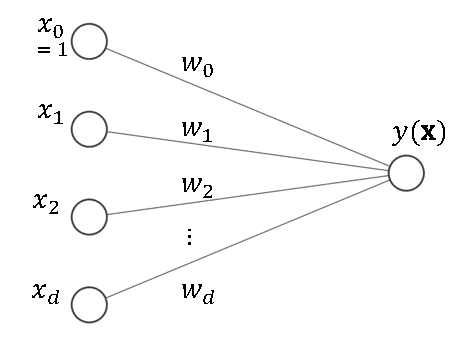
\includegraphics[width=\linewidth]{images/nn_perceptron.pdf}
        \caption{A computational graph of a standard perceptron. The input features $\mathbf{x}$ are linearly combined with the weights $\mathbf{w}$ and bias $w_0$ to produce the output $y$.}
        \label{fig:nn-perceptron}
    \end{subfigure}
    \hfill
    \begin{subfigure}[b]{0.45\linewidth}
        \centering
        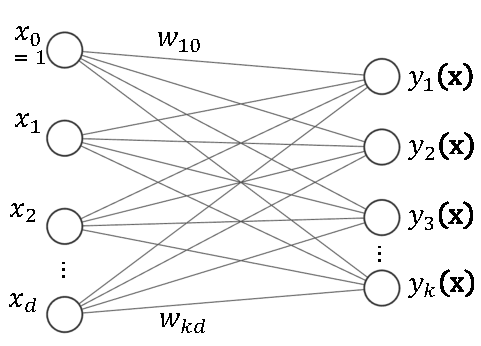
\includegraphics[width=\linewidth]{images/nn_multiclass.pdf}
        \caption{A computational graph of a multi-output perceptron. The input features $\mathbf{x}$ are linearly combined with the weights $\mathbf{w}$ to produce outputs $y_k$ for each dimension $k$.}
        \label{fig:nn-multiclass}
    \end{subfigure}
    \caption{Computational graphs for perceptron architectures. (a) Standard perceptron. (b) Multi-output perceptron.}
    \label{fig:nn-combined}
\end{figure}

\cref{eq:linear-regression} can be expressed as a computational graph, as shown in \cref{fig:nn-perceptron}. This architecture is commonly referred to as the standard perceptron, the simplest of neural networks.

\subsection{Generalization of Linear Models}
Linear regression can be extended to more complex settings, such as multi-output models (e.g.\ multi-class classification or multidimensional regression), with $y_k$ representing the output for the $k$-th dimension, and $x_0$ often set to $1$ as a convention for including the bias term $w_{k0}$:
\begin{equation}\label{eq:multi-output}
    y_k(\mathbf{x}) = \sum_{j=0}^{d} w_{kj} x_j
\end{equation}
Such an architecture is known as a single layer perceptron, and can be visualized as shown in \cref{fig:nn-multiclass}.

This can be further generalized by introducing non-linear basis functions $\phi_j(\mathbf{x})$, transforming the input features $\mathbf{x}$ before the linear combination:
\begin{equation}
    y(\mathbf{x}) = \sum_{j=0}^{d} w_j \phi_j(\mathbf{x})
\end{equation}
These non-linear transformations allow models to approximate non-linear relationships in data. Due to this, the loss can no longer be minimized in closed-form so iterative optimization algorithms such as gradient descent are used \cite{bishopPatternRecognitionMachine2006}.
Conventionally, these were basis functions were predefined and hand-crated based on domain knowledge, but we next look at deep learning models that can learn these basis functions.

\subsection{Deep Learning}
Multi-layer perceptrons build upon the foundations of linear models but eliminate the need to predefine input transformations. This is done by learning the parametrized basis functions from the data. 

One way to generalize the linear model is by applying a non-linear activation function $g$ to each input in \cref{eq:multi-output}. For example:
\begin{equation}
y_k(\mathbf{x}) = g\left(\sum_{j=0}^{d} w_{kj} x_j \right).
\end{equation}
To achieve this, neural networks add multiple layers to the computational graph, with each layer applying a linear transformation followed by a non-linear activation. A simple architecture is shown in \cref{fig:simple-nn-architecture} (with the addition of non-linearities), illustrating how the standard perceptron is extended to deeper networks.

Due to the non-linearities and layered structure, neural networks have high-capacity hypothesis spaces, suited to approximate the complex mappings such as multidimensional data such as images. 

\begin{figure}[h]
    \centering
    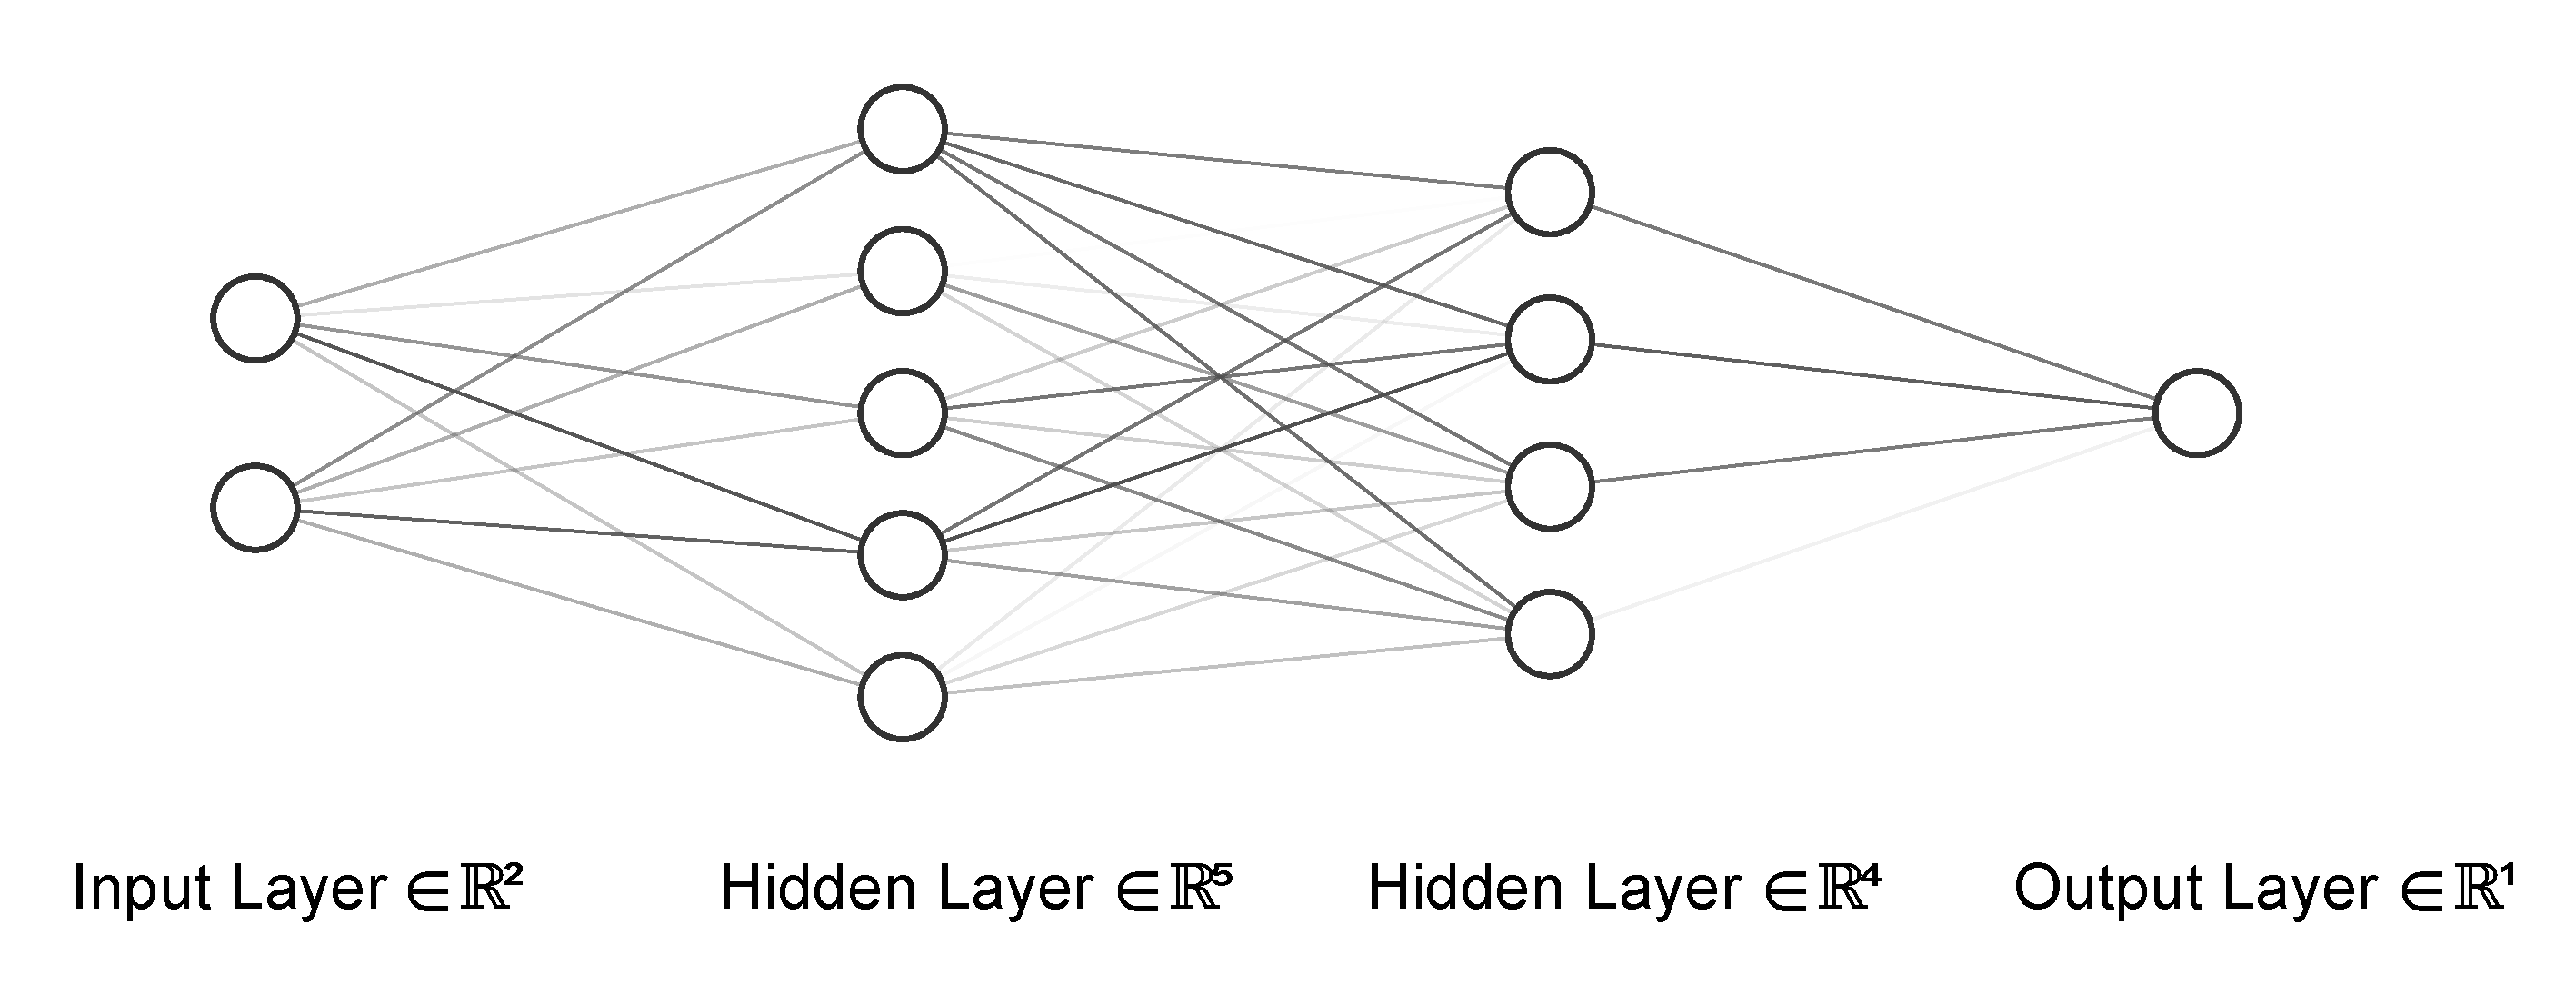
\includegraphics[width=1\linewidth]{images/simple_nn_architecture.pdf}
    \caption{An example trained fully connected neural network architecture with an input layer, two hidden layers, and an output layer. The input features are transformed through weights and biases, followed by a non-linear activation function in the first hidden layer. This process is repeated in the second hidden layer from outputs of the first (hidden) layer, producing the final outputs. The weights are represented by the lines connecting the neurons, with opacity indicating the weights' strength.}
    \label{fig:simple-nn-architecture}
\end{figure}

Activation functions are generally differentiable non-linear functions that introduce non-linearity into the network, allowing it to model complex relationships in the data. Common activation functions include the sigmoid function, that maps input values to a range between $0$ and $1$, useful to interpret probabilistically, and used in binary classification tasks. 
\begin{equation}
    S(x) = \frac{1}{1 + e^{-x}}
\end{equation}
Current state-of-the-art architectures often employ Rectified Linear Unit (ReLU) or its variants as the activation function, owing to their superior performance in training deep networks. ReLU defined as
\begin{equation}
    \text{ReLU}(x) = \max(0, x)
\end{equation}
sets negative inputs to zero while preserving positive inputs.

While ReLU is not differentiable at $x = 0$, it is widely favored due to its simplicity and effectiveness in training deep networks. Variants of ReLU, such as Leaky ReLU and Parametric ReLU have been introduced to address the issue of dead neurons, where neurons cease to learn during training. Leaky ReLU introduces a gradient for negative inputs
\begin{equation}\label{eq:leaky-relu}
    \text{Leaky ReLU}(x) = \max(\alpha x, x)
\end{equation}
defined by a small constant $\alpha$. Parametric ReLU extends this concept by allowing the gradient to be learned during training.

Training a neural network involves two primary phases: the forward pass and the backward pass. During the forward pass, the input data is propagated through the network, layer by layer, to generate an output. Following this, the backward pass occurs, in which the error, defined as the difference between the predicted output and the true output, is propagated back through the network using the gradient of the loss function. This step is crucial for updating the weights of the network.
The training process utilizes optimization algorithms, such as Stochastic Gradient Descent (SGD) \cite{sutskeverImportanceInitializationMomentum2013} or Adam Optimization \cite{kingmaAdamMethodStochastic2017}, which iteratively adjust the network's weights to reduce the loss.

\section{Neural Networks for Image Restoration using Noise2Noise Framework}
In the classical supervised-learning setting for image restoration, training assumes access to clean target images. Similar to \cref{sec:erm}, training can be formulated as
\begin{equation}
    \hat{h} = \argmin_{h \in \mathcal{H}} \frac{1}{\lvert \mathcal{S} \rvert} \sum_{(X, Y) \in \mathcal{S}} \ell(h(X; \theta), Y),
\end{equation}
where $\mathcal{S} \sim \mathcal{D}^n$ is the training set with images $\mathcal{S} = \{(X_1, Y_1), \dots, (X_n, Y_n)\}$ with $(X, Y)$  the noisy and clean target images.

Most often, instead of a multilayered perceptron architecture, \gls{CNN} are preferred for image restoration tasks. \gls{CNN} are well-suited for image data due to their ability to learn spatial hierarchies of features through convolution operations. he convolutional layers in a \gls{CNN} automatically detect patterns such as edges, textures, and shapes, while the pooling layers downsample the data to reduce both the number of parameters and computational complexity. The output of the convolutional layers, known as feature maps, captures these learned patterns, and max-pooling further enhances efficiency by retaining the most significant values in a region, reducing spatial dimensions. This pooling process also contributes to the network’s robustness to spatial variance. Furthermore, \glspl{CNN} impose a strong prior on the hypothesis space, assuming that the data is translationally invariant, which is a reasonable assumption for images \cite{goodfellowDeepLearning2016}. In the context of this work, we will explore a specific realization of \glspl{CNN}, namely the UNet, which is known for its effective use in image restoration tasks.

In many practical scenarios such as our \gls{MPES} data, obtaining the true clean image $Y$ is not feasible, although sufficiently high quality noisy data exists. In the instance when multiple noisy realizations of the same underlying signal are available, \citeauthor{lehtinenNoise2NoiseLearningImage2018} demonstrated that it is possible to train a neural network to learn a restoration mapping to the underlying clean signal using only noisy observations for both inputs and targets \cite{lehtinenNoise2NoiseLearningImage2018}, a framework known as \textit{Noise2Noise}. 

In the following sections, we see why Noise2Noise works and how it is applied to our image restoration problem.
\subsection{Point Estimation and Loss Functions}
We discussed in \cref{sec:generalization} that we aim to learn a hypothesis that generalizes to new data coming from the distribution $\mathcal{D}$. This can be done by minimizing the risk (\cref{eq:risk-min}). 

Consider an example point estimation problem where the objective is to find the scalar $\hat{x}$ that minimizes the expected deviation with respect to a set of observations $x_1, x_2, \dots, x_n$. This can be formalized as:
\begin{equation}
    \hat{x} = \argmin_{\hat{x}} \mathbb{E}[\ell(\hat{x}; x)]
\end{equation}
Different loss functions yield varying estimates based on the observations. For the case of $L_2$ loss, the minimization recovers the mean of the observations:
\begin{equation}\label{eq:l2-estimate}
    \hat{x} = \mathbb{E}[x]
\end{equation}
Similarly, for the $L_1$ loss, the estimate is the median of observations.

\subsection{Zero-Mean Noise}
Combining \cref{eq:risk} and \cref{eq:risk-min}, we can write the risk minimization problem as:
\begin{equation}
    \argmin_{h \in \mathcal{H}} \mathbb{E}_{x \sim \mathcal{D}} \left[\mathbb{E}_{y|x \sim \mathcal{D}} \left[ \ell(h(x; \theta), y) \right]\right]
\end{equation}
where using the law of total probability, the joint expectation $p(x,y)$ can be factorized to $p(x) \cdot p(y | x)$, and hence the expectation as well. This formulation is equivalent to solving the point estimation problem for each input sample separately. Due to this, the neural network inherits the properties of the loss function.

We established in \cref{eq:l2-estimate} that minimizing the $L_2$ loss recovers the mean of the observations. Now, consider the case where the training targets $y$ are corrupted with zero-mean noise, $\mathbb{E}[n] = 0$. The expectation remains unchanged i.e.\ $\mathbb{E}[y] = \mathbb{E}[x^\prime|y]$, with $x^\prime$ being the corrupted data. For example, we previously demonstrated Poisson noise being zero-mean  in \cref{sec:poisson-noise-model} (see \cref{eq:poisson-noise,eq:zero-mean-noise}), and hence, the $L_2$ loss could also recover, on expectation, the true value of a Poisson noise corrupted variable. Using other losses such as $L_1$ could allow recovery of signals with significant outlier content.

This principle can extend to neural network training as we already said that the network inherits the properties of the loss. When minimizing the risk, a neural network trained with zero-mean noise-corrupted targets will converge to the same optimal hypothesis as it would with clean targets. This holds true in the context of \gls{ERM} as well. With infinite training data, minimizing the empirical risk using noisy observations is mathematically equivalent to minimizing it with clean targets (\cref{eq:erm}).

\subsection{Noise2Noise Training for Finite Data}
Let us formalize the Noise2Noise training for a realistic case of finite examples. Consider a training set $\mathcal{S}^\prime = \{(X_1, X_1^\prime), \dots, (X_n, X_n^\prime)\}$ where $\mathcal{S}^\prime \sim \mathcal{D}^n$, each pair $(X, X^\prime)$ independent noisy realizations of the same underlying signal $y \sim \mathcal{D}$. Using the $L_2$ loss, we can redefine \gls{ERM} formulation from \cref{sec:erm} as
\begin{equation}\label{eq:erm-noise2noise}
    \hat{h} = \argmin_{h \in \mathcal{H}} \frac{1}{\lvert \mathcal{S^\prime} \rvert} \sum_{(X, X^\prime) \in \mathcal{S}^\prime} (h(X; \theta) - X^\prime)^2
\end{equation}
giving us a hypothesis $\hat{h}$ that minimizes the training error using only noisy observations for both inputs and targets.

For finite data, the quality of the estimate depends on the variance of the noise in the targets, divided by the number of samples $N$ \cite[supplementary~material]{lehtinenNoise2NoiseLearningImage2018}. This means that increasing the dataset size reduces the variance of the estimate, bringing it closer to the hypothesis had we minimized with clean targets. For image data, $N$ corresponds to the total number of scalar components\footnote{Number of images $n$ x number of voxels per image x number of color channels.} across the dataset, so having more voxels and data effectively brings us closer to the infinite data case.

\subsection{Regularization through Noisy Targets}
It is important to note that the earlier discussion assumed that learning with clean targets is inherently successful, while in fact, as we discussed before, \gls{ERM} is prone to overfit (generalizes poorly) in high-capacity hypothesis spaces. Using noisy targets actually has the unexpected benefit to act as a form of regularization. The noise in the targets perturbs the training objective, preventing the network from relying excessively on precise input-output mappings. For image restoration tasks, this can lead to better generalization, as the network focuses on recovering the underlying clean signal structure rather than spurious details in the data.

\section{Training an MPES Denoiser}
As seen in \cref{sec:image-formation}, the experimental setup (refer to \cref{section:hextof,section:dld}) for \gls{MPES} puts us in a unique position of having access to multiple noisy realizations of the same underlying image. This allows us to generate training data pairs where both the input and target are noisy versions of the same image. We can hence leverage the Noise2Noise \gls{ERM}, as shown in \cref{eq:erm-noise2noise}, to train a neural network to denoise \gls{MPES} images. We perform all the shown experiments with the $L_2$ loss\footnote{Some preliminary study using the $L_1$ loss also shows promise. This could be attributed to the significantly high noise at low count levels.} as the underlying images we aim to recover are the expectation of the noisy images.

Selecting the training data and neural network architecture are imperative for the success of the denoising task. Given the inherently multidimensional nature of \gls{MPES} data, it is advantageous to exploit cross-dimensional correlations to better estimate the underlying image. While 2D image restoration methods already utilize such principles in two dimensions, an example we already discussed with \gls{BM3D} in \cref{sec:bm3d}, higher dimensional data can provide additional information to improve the denoising performance\footnote{Algorithms such as BM4D \cite{maggionimNonlocalTransformdomainFilter} attempt to exploit this by considering the 3D structure of the data.}. 

This is further necessary since the 2D image slices from even our best dataset (\gls{ncounts} of \num{1.86e8} from \gls{GrIr}) are still noisy. In fact, in \cref{sec:mpes-bm3d-denoise}, we employed slice summing before denoising and also in evaluation. However, this summation leads to feature blurring and harnessing correlations across higher dimensions provides a more effective alternative.

To this end, we employ the UNET3D architecture, utilizing 3D convolutions, upsampling and pooling, instead of their 2D counterparts. In the following, we detail the data generation process, network architecture and the training and validation schemes.

\subsection{Training Data Generation}
\begin{figure}[h]
    \centering
    \begin{subfigure}[t]{0.59\linewidth}
        \centering
        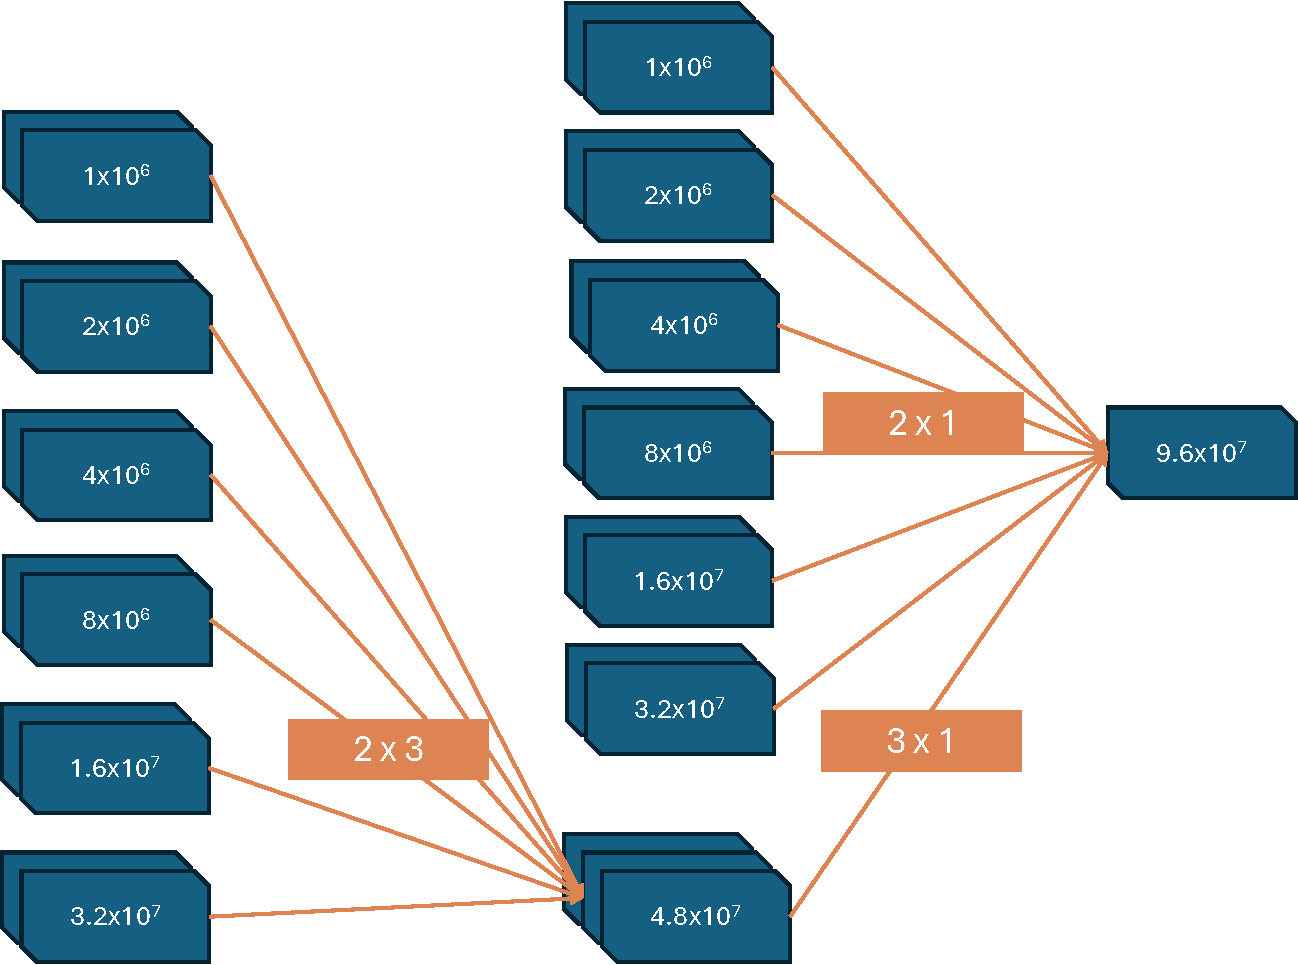
\includegraphics[width=1\linewidth]{images/training_flowchart.pdf}
        \caption{Flowchart illustrating the input-target dataset pairs, derived from subsets of the \gls{GrIr} dataset. A total of \num{34} unique noisy datasets are represented, with each dataset corresponding to one blue box in the chart. The different combinations shown in the chart generate \num{51} input-target pairs across counts \numrange{1e6}{9.6e7}.}
        \label{fig:training-data-flowchart}
    \end{subfigure}
    \hfill
    \begin{subfigure}[t]{0.39\linewidth}
        \centering
        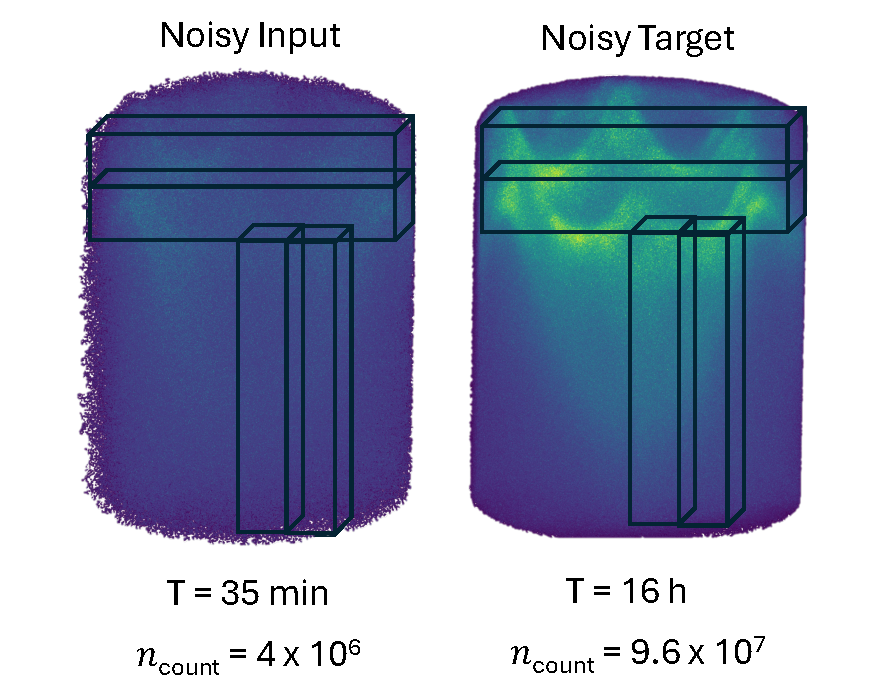
\includegraphics[width=1\linewidth]{images/training_3d_patch_example.pdf}
        \caption{Showing example noisy input and noisy target and how 3D subsets (also called patches) are extracted for training. On top, how extracted subsets could look.}
        \label{fig:training-3d-patch-example}
    \end{subfigure}
    \caption{Illustration of generating neural network training pairs. (a) The flowchart showing the input-target dataset pairs used for training, and (a) an example of noisy input and noisy target showing how 3D subsets are extracted from the volume. Through the combination with patch-based extraction, a total of \num{5967} training pairs are generated. The \num{4.8e7} and \num{9.6e7} counts serve as the target datasets, with \num{9.6e7} additionally functioning as the target for the \num{4.8e7} datasets.}
\end{figure}
The \gls{GrIr} dataset, with its high count, is used as the training dataset. While Noise2Noise training allows training with noisy data, it is not immediately apparent at what noise levels the training should be conducted. Naturally, the noise levels we aim to denoise should be reflected in the training set. Of particular interest are datasets obtained with shorter acquisition times $T$, and thus lower \gls{ncounts}. The authors in \cite{lehtinenNoise2NoiseLearningImage2018} demonstrated succesful training and inference on Poisson corrupted images with $\lambda \in [1, 50]$. Assuming Poisson noise\footnote{Which we know not to be the case from \cref{ch:pes-statistics}, but 
sufficies for the current argument.}, for our lowest-count noisy dataset, which has an average count per voxel of \num{5.98e-3}, and even our highest count dataset (\num{1.13} per voxel; see \cref{noisy-dataset-table}), the noise levels lie largely outside the range previously studied. Only the highest count dataset aligns with their researched range.

Hence, we go for the range that is most interesting for us, with inputs spanning \numrange{1e6}{4.8e7} and targets using \num{4.8e7} and \num{9.6e7}. To make this problem tractable and given the constraint of having independent datasets, a limited number (\num{34}) of input-target image pairs are used, as seen in \cref{fig:training-data-flowchart}. 

The ideal situation is if we have independent noisy dataset realizations. For instance, \num{1e6} \gls{ncounts} should not be sampled from the same region which is a subset of a \num{2e6} dataset, as overlapping events would introduce dependencies between datasets. While achieving complete independence is straightforward for lower-count datasets, it becomes increasingly challenging when sampling from the highest \gls{ncounts} of \num{1.86e8}. To mitigate this issue, we avoid using the maximum \gls{ncounts} during training, increasing the independence of datasets. 

Prior work by \citeauthor{lehtinenNoise2NoiseLearningImage2018} demonstrated that using cleaner targets, even with fewer noisy realizations (e.g., just two), significantly enhances denoising performance. Future improvements could involve incorporating other \gls{MPES} datasets to increase the pool of independent images. Additional studies could also examine whether including partially dependent datasets improves denoising performance.

We employ a patch-based approach to getting training pairs. Firstly, to increase the training data, having many independent training pairs, and secondly to make the problem computationally feasible, as training on entire 3D volumes would be prohibitively expensive, making batch-based training challenging. We extract 3D patches from the 3D volumes, as shown in \cref{fig:training-3d-patch-example}, generating \num{5967} training pairs. The patches are extracted at $60 \times 240 \times 240$ size, with a stride of $30 \times 120 \times 120$. The patches are then normalized to have zero mean and \numrange{-1}{1} ranges, common preprocessing step that centers the data and enhances neural network learning performance \cite{bishopDeepLearningFoundations2024}. 

To further augment the data, random rotations and flips are applied to the extracted patches. This augmentation not only increases the variability in the training data but also helps the neural network generalize better during inference.

\subsection{Model Architecture: UNET3D}
\begin{figure}
    \centering
    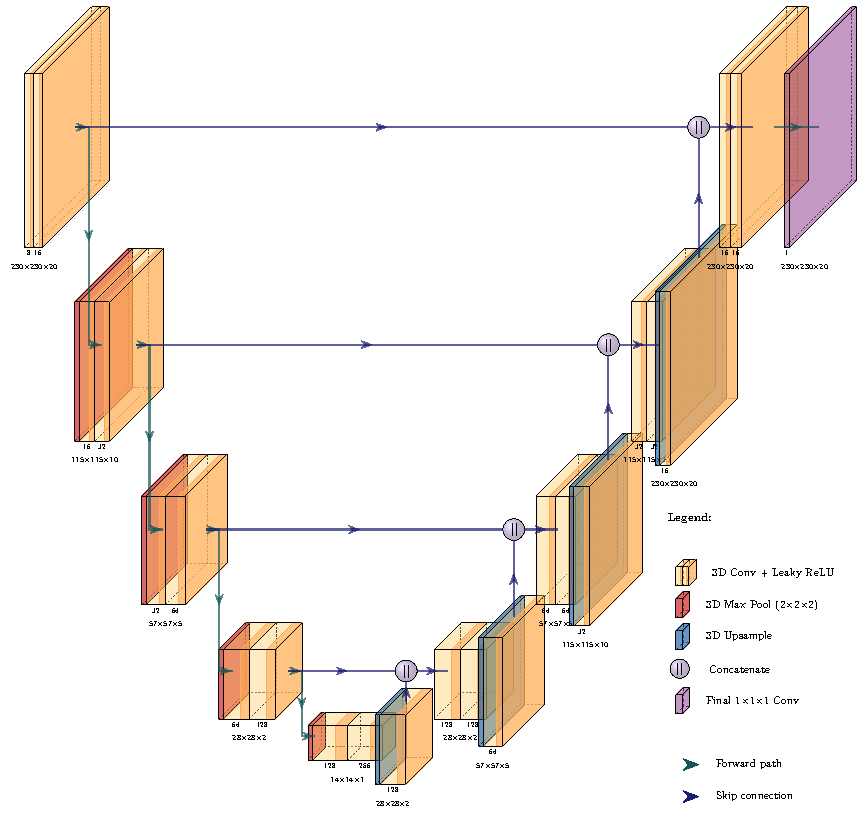
\includegraphics[width=0.8\linewidth]{images/unet_architecture.pdf}
    \caption{UNET3D architecture used for training the neural network, with example inputs propogated through the network. The architecture consists of an encoder-decoder structure with skip connections. The encoder compresses spatial information using a series of convolutional layers and 3D max-pooling operations, while the decoder reconstructs the data to its original dimensions using upsampling layers and convolutional operations. Skip connections link corresponding encoder and decoder levels, allowing feature reuse and aiding gradient flow during training.}
    \label{fig:unet-architecture}
\end{figure}

While in principle any denoising \gls{CNN} architecture could be used, we employ the UNET architecture, a popular choice for image restoration tasks, especially in medical imaging, where it has shown remarkable success \cite{ronnebergerUNetConvolutionalNetworks}. We extend the UNET architecture to train 3D data using 3D patches \cite{cicek3DUNetLearning2016}. Due to its relatively shallow architecture in comparison to deeper models, UNET accelerates the 3D learning process.

The name, UNET, takes after the architecture’s structure, a distinctive “U-shaped”, as illustrated in \cref{fig:unet-architecture}. UNET, similar to an autoencoder, consists of an encoder-decoder structure, forming the left and right halves of the “U-shape”. The difference from traditional autoencoders is the presence of skip connections (purple arrow) that link corresponding encoder and decoder levels. These connections allow the network to reuse features from the encoder during the decoding process, aiding gradient flow during training. The skip connections are also particularly useful in recovering fine-grained details lost during downsampling in the encoder.

The encoder compresses spatial information using a series of convolutional layers and 3D max-pooling operations. This progressively reduces the spatial dimensions while increasing the feature channels. On the other hand, the decoder reconstructs the data to its original dimension using upsampling layers and convolution operations. 

The model leverages 3D convolutions, allowing it to capture spatial features across the depth, height, and width dimensions simultaneously. Downsampling within the encoder is achieved through 3D max-pooling layers $2 \times 2 \times 2$ kernels, while the decoder employs 3D upsampling to restore spatial dimensions. The input data is processed in patches of size $60 \times 240 \times 240$ voxels\footnote{This is just how we train the data but \glspl{CNN} can process any arbitrary resolution, provided sufficient memory. In fact, during inference, we employ a larger patch size.}, which are reduced and then restored in the encoder-decoder pipeline. As illustrated in \cref{fig:unet-architecture}, intermediate feature maps progressively decrease in spatial dimensions (e.g., $230 \times 230 \times 20 \to 115 \times 115 \times 10 \to 57 \times 57 \times 5$) in the encoder and are restored in reverse order in the decoder. \todo{write about fmaps [16, 32, 64, 128, 256]}

The model uses Leaky ReLU activation functions, as seen in \cref{eq:leaky-relu}, with a negative slope of 0.01, which enhances gradient flow in regions with low activation values. Within each feature channel, group normalization (of size 8) is employed to improve training stability and performance. Group normalization performs normalization independent of the batch sizes by dividing the channels into groups and computing the mean and variance within each group across the channels. However, Batch Normalization calculates the mean and variance across the whole batch for every channel of features and is suited for larger batch sizes.

Additionally, due to memory limitations, we use a batch size of \num{16}. Hence, within each feature, group normalization (of size 8) is applied here instead, since batch normalization is known to be unstable, particularly for small batch sizes. Group normalization performs normalization independent of the batch sizes by dividing the channels into groups and computing the mean and variance within each group across the channels \cite{wuGroupNormalization2018}. However, Batch Normalization calculates the mean and variance across the whole batch for every channel of features and is suited for larger batch sizes.

The final layer of the network consists of a $1 \times 1 \times 1$ convolution, which maps the feature space to a single output channel, producing the denoised result.


\subsection{Training and Validation}
\begin{figure}
    \centering
    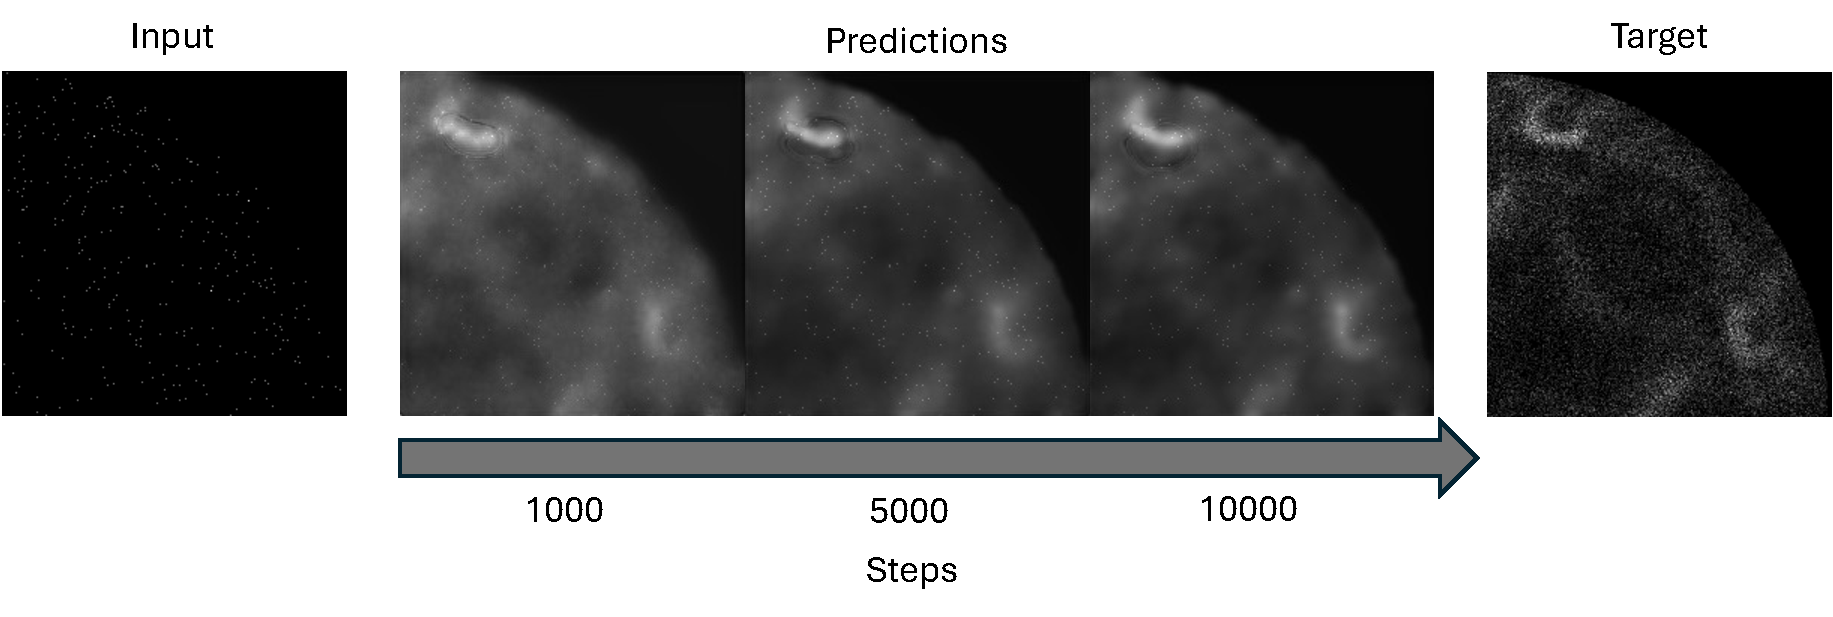
\includegraphics[width=1\linewidth]{images/training_progress_example2.pdf}
    \caption{Denoising predictions at step \numlist{1000;5000;10000} during training are shown, along with the input and target images. The key features, though blurry, are quickly discernible in the denoised images, even at early stages of training.}
    \label{fig:training-progress-example}
\end{figure}
For training, the model is optimized using the Adam optimizer with an initial learning rate of \num{0.001} and beta values of \num{0.9} and \num{0.99}. The learning rate is adjusted dynamically using a \texttt{ReduceLROnPlateau} scheduler, which reduces the rate by a factor of \num{0.1} if the primary evaluation metric does not improve for \num{10} validation runs. The training is conducted with a batch size of \num{16}, for a maximum of \num{1e3} epochs or until \num{1e5} iterations are completed. Validation is performed every \num{1e3} iterations using \gls{SSIM} as the primary metric and \gls{PSNR} as evaluation metrics. This training was performed prior to the results regarding \gls{MSSSIM} in \cref{sec:metric_comparison_experiment}. Therefore, while \gls{SSIM} was used here, a better validation could be obtained using \gls{MSSSIM} in future work.

For validation, we split our 3D dataset with a 80-20 ratio along the $E$ dimension, with the first 80\% used for training and the remaining 20\% for validation. Most of the key features exist in the training set but due to limited data availability, we can only employ low quality features for validation. We use the highest count dataset to validate against. The validation set is used to monitor the model's performance and prevent overfitting. 

Checkpoints are saved after every validation run, enabling resumption from the last checkpoint if interrupted. Furthermore, the model with the best validation \gls{SSIM} score is saved separately. The training progress for a single (training) example is shown in \cref{fig:training-progress-example}, where the denoising performance shows perceptually significant improvements already at early stages of training.



\begin{figure}
    \centering
    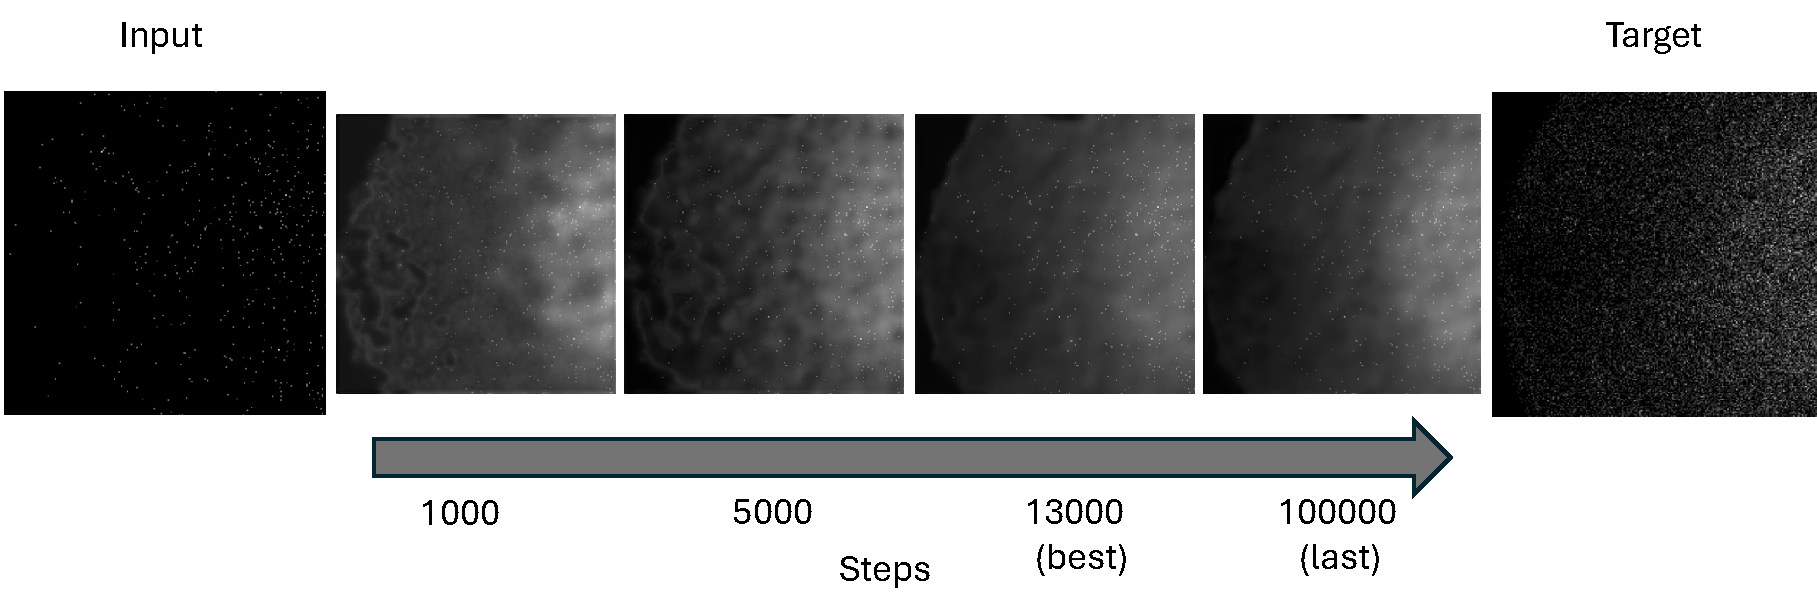
\includegraphics[width=1\linewidth]{images/val_over_time.pdf}
    \caption{Denoising predictions at step \numlist{1000;5000;13000;100000} during validation are shown, the latter two of which correspond to the best and last models. The input and target images are also shown. The validation set features not as discernible as the training set, as they correspond to energies much above the Fermi level.}
    \label{fig:val-progress-example}
\end{figure}

The training and validation loss are shown in \cref{fig:loss-training-val}. It has already been exemplified in \cite{lehtinenNoise2NoiseLearningImage2018} that the training loss does not decrease during training, as the network can not possibly learn to transform one instance of noise to another, as the training asks for the impossible. Hence, other than the initial decrease, the network loss stays plateaued consistently across \num{1e5} steps. However, since our validation target is a higher quality noisy dataset \num{1.86e8}, the expectation would be that it reports higher loss values. But as we discussed earlier, the validation set data is much above Fermi level, with features indistinguishable. The validation loss can be seen to converge to a stable value at \num{4e4} steps. 

\begin{figure}
    \centering
    \begin{subfigure}[t]{0.49\linewidth}
        \centering
        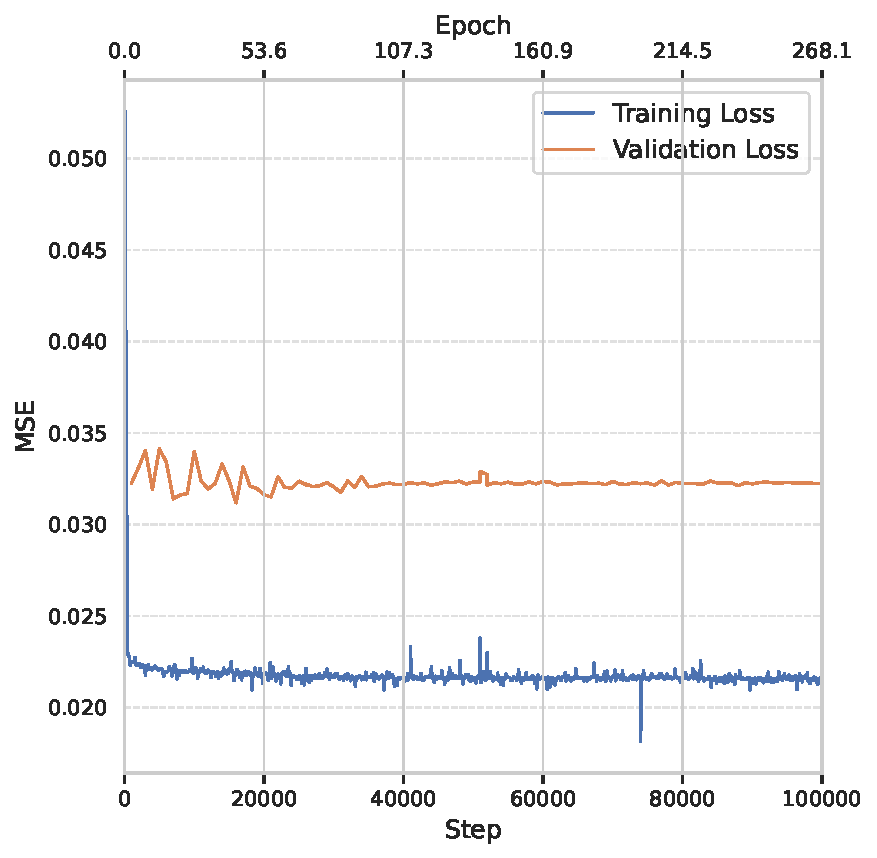
\includegraphics[width=1\linewidth]{images/loss_training_val.pdf}
        \caption{Training and validation loss. The gap exists due to the validation set being compared with higher quality targets. The validation loss converges to a stable value at \num{4e4} steps.}
        \label{fig:loss-training-val}
    \end{subfigure}
    \hfill
    \begin{subfigure}[t]{0.49\linewidth}
        \centering
        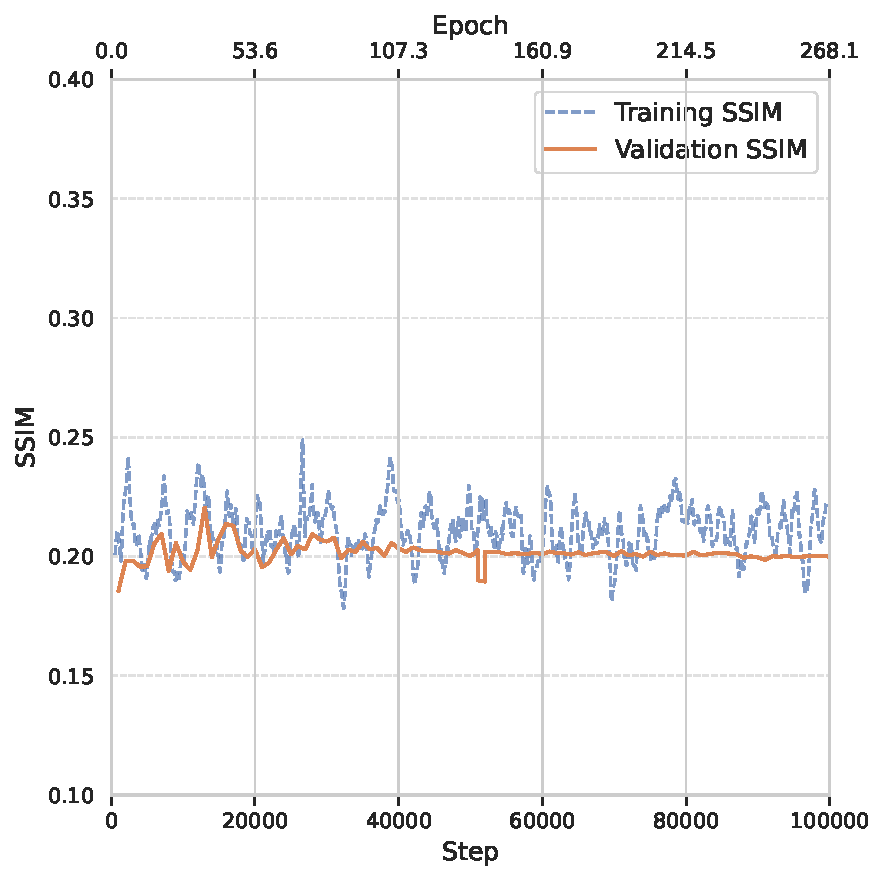
\includegraphics[width=1\linewidth]{images/ssim_training_val.pdf}
        \caption{\gls{SSIM} scores across training and validation. The scores show constant fluctuations around an average value during training but show less fluctuations during validation, where validation also converges to a stable value at \num{4e4} steps.}
        \label{fig:ssim-training-val}
    \end{subfigure}
    \caption{(a) Training and validation loss and (b) \gls{SSIM} scores over training steps and epochs. The UNET3D architecture is trained, using noisy input-targets pairs.}
    \label{fig:loss-ssim-training-val}
\end{figure}

The metric assessment using \gls{SSIM}, shown in \cref{fig:ssim-training-val}, also shows constant fluctuations around an average value in during training but are shown to be converging in the validation. We therefore look at two models, the (\textit{best}) model with the highest validation \gls{SSIM} of \num{0.23} that happens early on during training, after about \num{25} epochs\footnote{Meaning we do \num{25} passes of our entire dataset during training.}, and the (\textit{last}) model at end of training, where the validation \gls{SSIM} has converged to \num{0.2}.

\begin{figure}
    \centering
    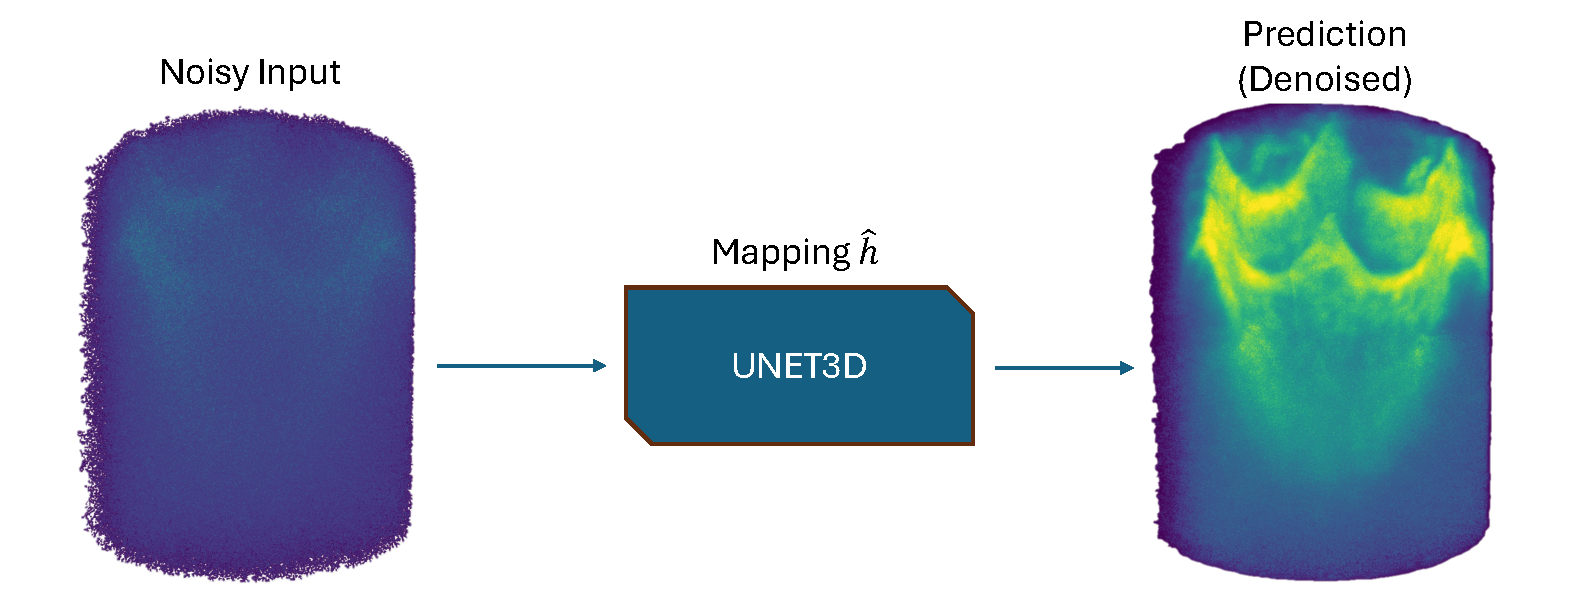
\includegraphics[width=1\linewidth]{images/noisy_denoised_3d.pdf}
    \caption{Example prediction (forward pass) from \num{4e6} count dataset, using the best model The prediction resolves the key features in the noisy input, showing the effectiveness of the denoising model.}
    \label{fig:3d-image-noisy-denoised-training}
\end{figure}

\begin{figure}
    \centering
    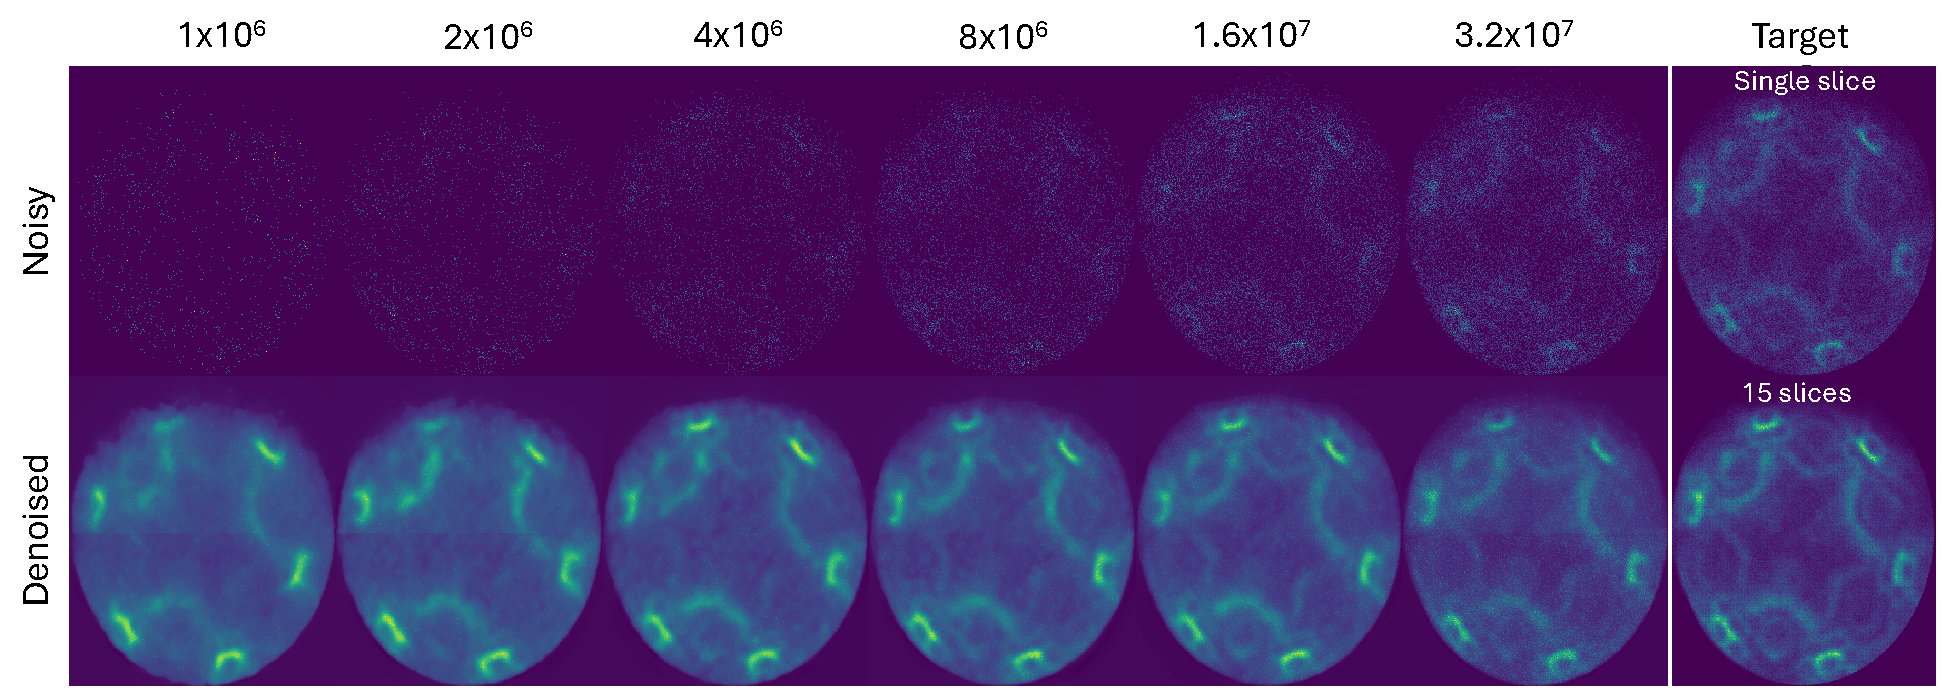
\includegraphics[width=1\linewidth]{images/images_noisy_denoised_with_target.pdf}
    \caption{Noisy and denoised \gls{ky}-\gls{kx} cuts with window size $w=1$ shown for \gls{GrIr} dataset. Each column corresponds to \numlist{1e6;2e6;4e6;8e6;1.6e7;3.2e7;1.86e8} counts, respectively; where the last column is the target image with $w=1$ in row 1 and $w=15$ in row 2. Below \num{8e6} counts, none of the features are discernible for noisy images, while the denoised images show clear features similar to the target.}
    \label{fig:images-noisy-denoised-training}
\end{figure}

\cref{fig:3d-image-noisy-denoised-training} illustrates how the mapping $\hat{h}$ learned during training predicts data. Looking at \cref{fig:images-noisy-denoised-training}, we see the noisy and denoised \gls{ky}-\gls{kx} cuts for the \gls{GrIr} dataset, at different noise (count) levels. The noisy images show no discernible features below \num{8e6} counts, while the denoised images show clear features similar to the target. The model evaluated on the training set hence shows promising results. To really be sure that the model achieved generalized capability of denoising the experimental data, and not just learned the features of the training set, we need to evaluate it on independent test data.



\subsection{Evaluating Model Denoising Performance}
\begin{figure}
    \centering
    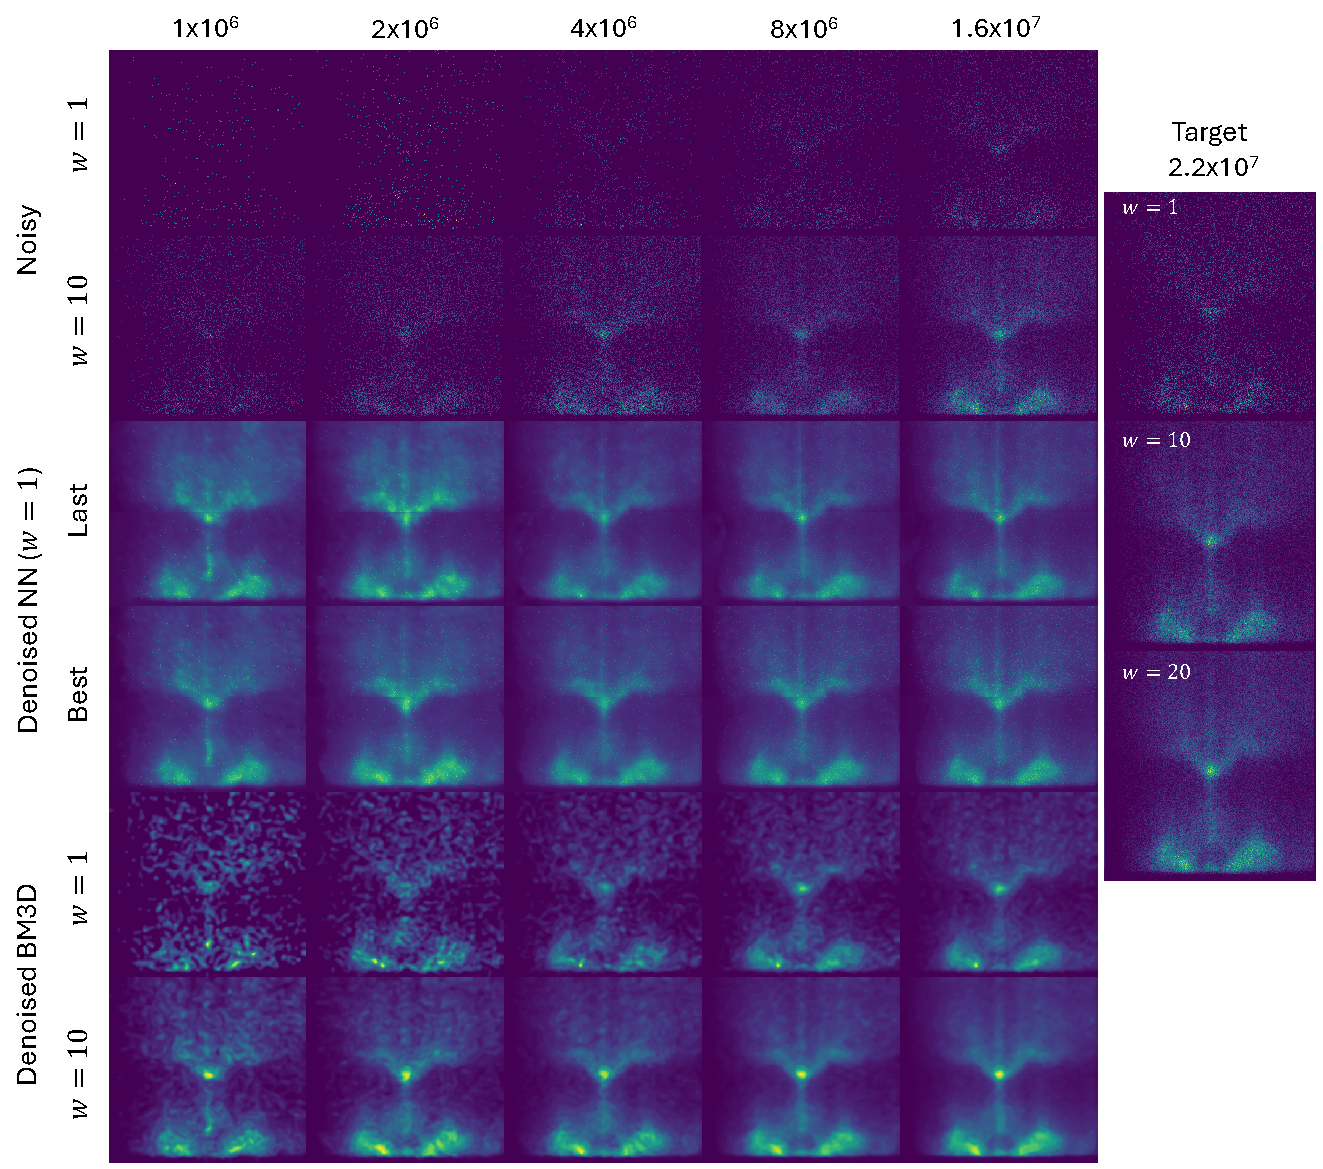
\includegraphics[width=1\linewidth]{images/nn_denoised_counts_best_last_ex_bm3d.pdf}
    \caption{Comparison of \gls{kx}–\gls{E} slices for various \gls{ncounts}. The target image is shown for a single slice and for slice-summed images with \gls{winsize} values of \num{10} and \num{20}, demonstrating the effect of summing slices for visual quality improvement. The noisy image is also depicted as a slice-summed result, emphasizing that slice summing acts as a basic form of noise reduction. Denoised results are shown for the best and last trained neural network models ($w=1$), alongside \gls{BM3D}–Anscombe denoising applied with the optimal parameter $\sigma_{\text{o}}$ for $w=10$ and the same parameter used for $w=1$. The results illustrate that the neural network outperforms BM3D–Anscombe denoising at lower counts (\num{1e6}). At higher counts and when slices are summed, BM3D’s performance improves relative to the neural network.}
    \label{fig:nn-denoised-counts-best-last-ex-bm3d}
\end{figure}

We use the \gls{GdW} dataset for evaluating the model's generalization capability. \cref{fig:nn-denoised-counts-best-last-ex-bm3d} shows a \gls{kx}--\gls{E} slice for noisy and denoised images for best and last models, as well as comparison with \gls{BM3D}--Anscombe denoising. The plot also show the slice summed image with \gls{winsize} of \num{10} for noisy image, that also acts as some sort of denoising. BM3D results are also shown for this sum as for lower counts, BM3D performs poorly. \cref{fig:nn-denoised-counts-best-last-xy-bm3d} shows the \gls{ky}--\gls{kx} slice for the same models and \gls{BM3D}--Anscombe denoising.

From this it can be understood that neural network based denoising performs much better at lower counts (even at \num{1e6}) than BM3D based denoising. At higher counts and summed slices, the BM3D denoising also perform well, a conclusion we already drew in \cref{ch:datasets_bm3d}. To see if slice summing has any improvement in denoising performance of the neural network, one can look at  \cref{fig:nn-denoised-counts-best-last-xy-bm3d-slice-sum-last-model}, showing the last model denoising performance on the summed slice. The denoising performance is not improved by the slice summing, as the features are already well resolved in the individual slices. As before, this leads to feature blurring and for the neural network model, is not leading to any significant perceptual improvement. This can be explained by the fact that my using a 3D model, we have already taken into account the correlations across the depth dimension, and hence the slice summing does not provide any additional information.

\begin{figure}
    \centering
    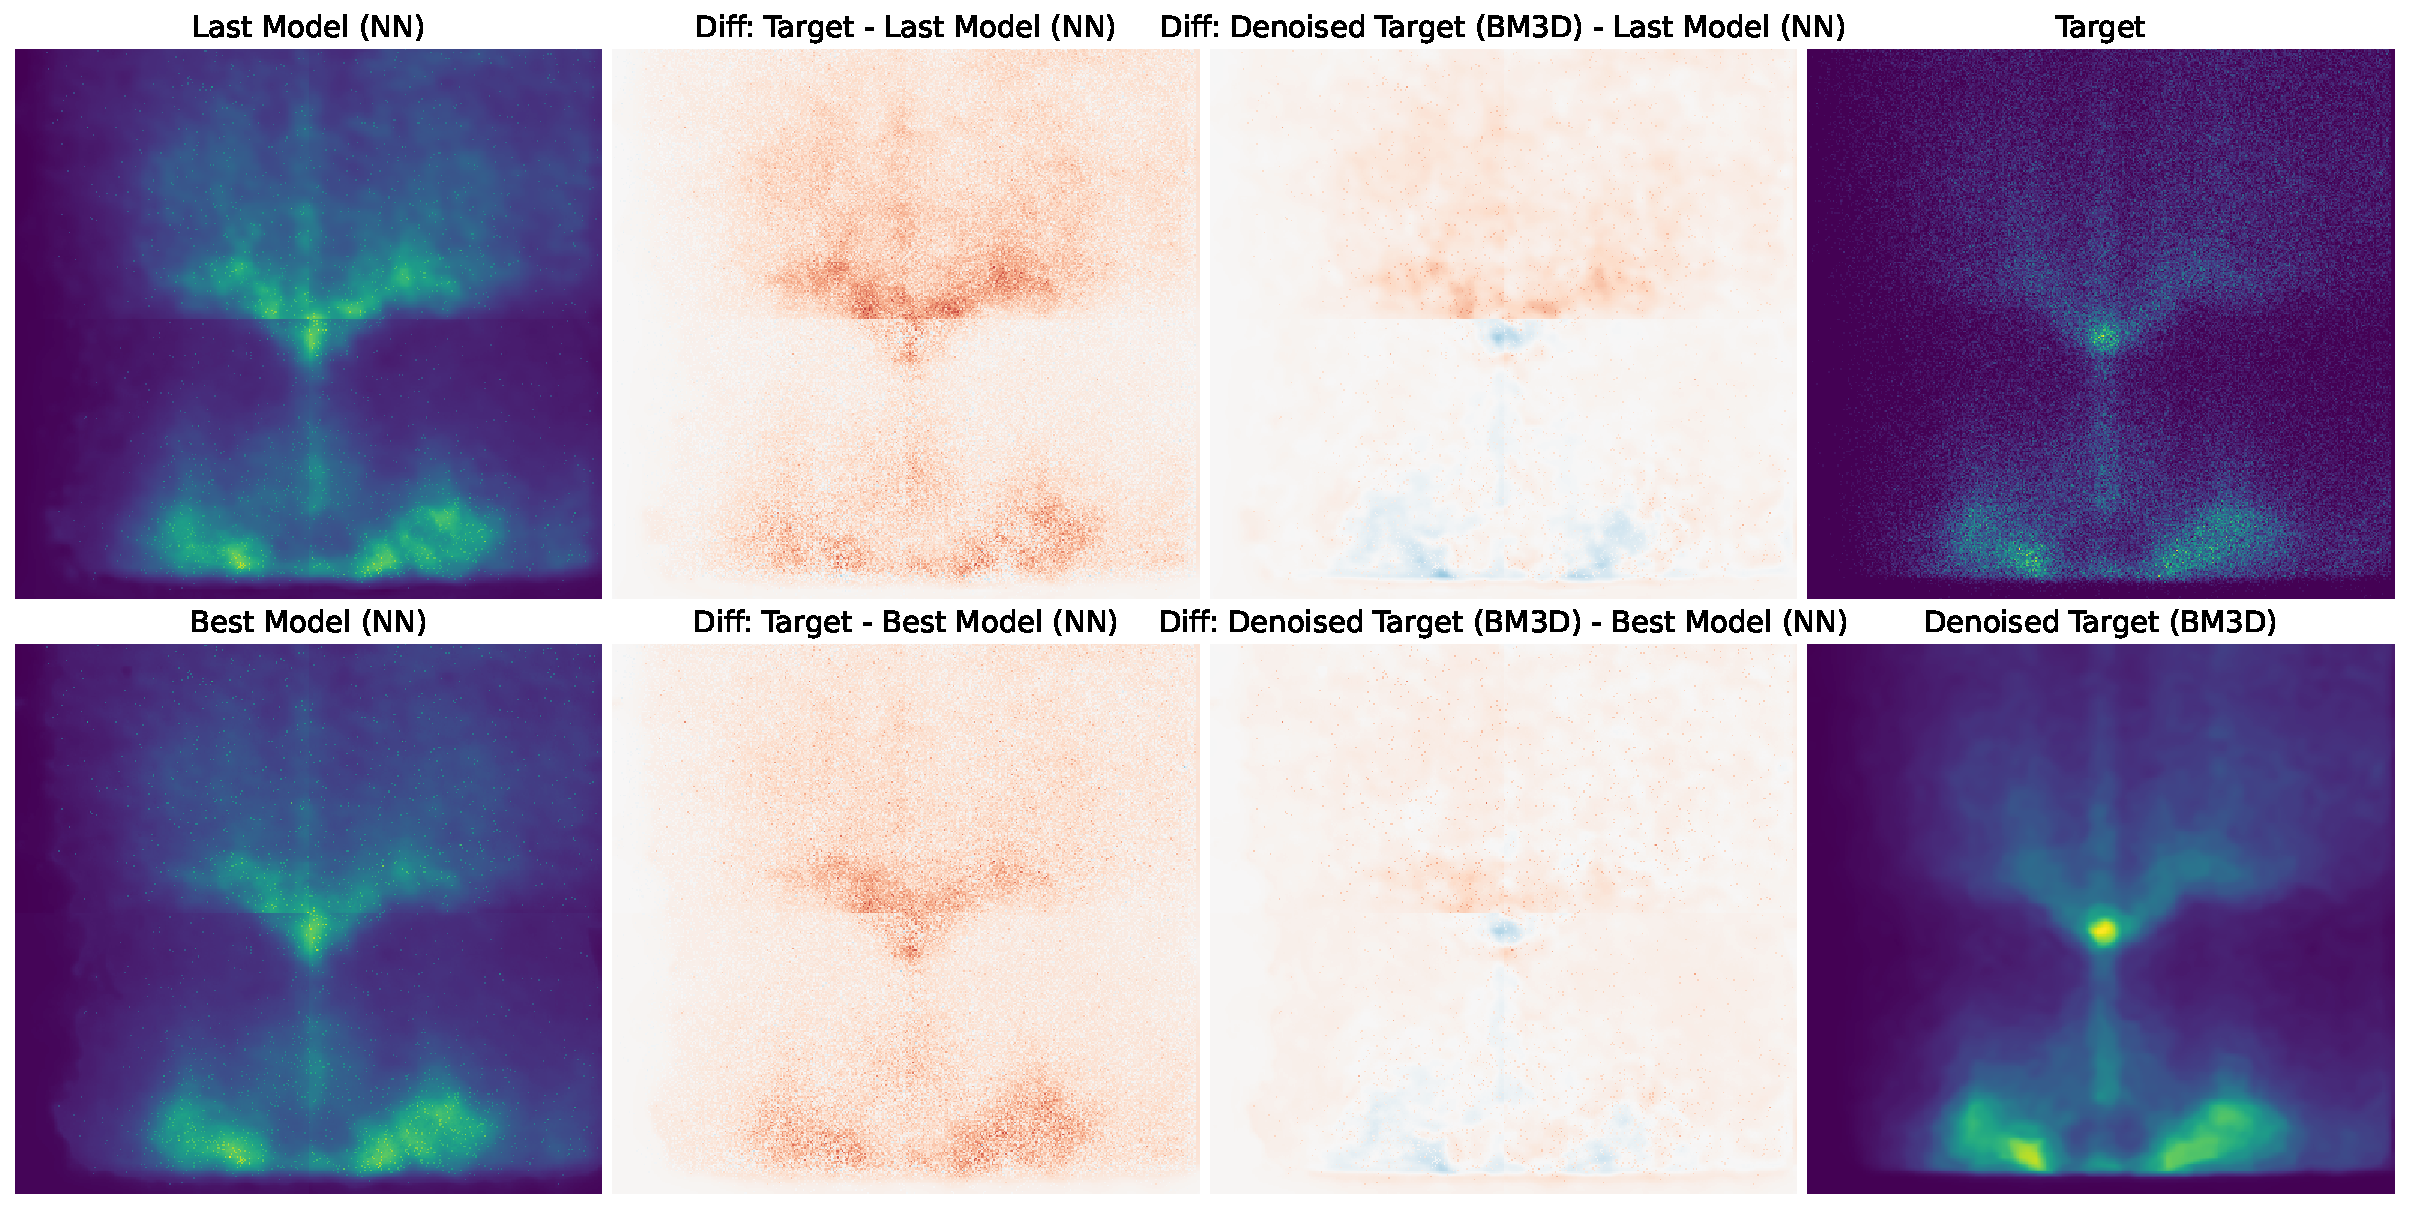
\includegraphics[width=1\linewidth]{images/nn_diff_plots_2M.pdf}
    \caption{Difference images comparing the best and last models for \gls{ncounts} \num{2e6}. The differences are computed relative to two references: the slice-summed target image with \gls{winsize} of \num{10}, and its BM3D-denoised version. The red regions indicate where the prediction is brighter than the noisy target, while blue regions indicate where the target is brighter. The target itself is noisy, so when subtracting the denoised outputs from the target, mostly red regions are visible. However, when using the BM3D-denoised target as a reference (assumed to approximate the correct image), the differences are mostly white (close to 0), with some blue regions where predicted features are less intense compared to the reference. These difference plots highlight that the best model preserves features more effectively and aligns better with the BM3D-denoised target compared to the last model.}
    \label{fig:nn_diff_plots_2M} 
\end{figure}

Let us now explore whether the longer training time to obtain the last model is worthwhile, since the best model is obtained early on. To explore this,  we can look at the difference images between the predicted output and target image. Since the target is noisy, we look at slice summed images with \gls{winsize} of \num{10} to get a better idea of the features. Furthermore, we also compare the best and last models with a BM3D denoised target image. Since BM3D is performing well at these counts, it can be used as a reference for the neural network denoising performance.

The difference images are shown in \cref{fig:nn_diff_plots_2M} and \cref{fig:nn_diff_plots_8M} for \num{2e6} and \num{8e6} counts, respectively. Comparing with the target, both models show unsharp features at \cref{fig:nn_diff_plots_2M}, especially the last model. Whereas, \cref{fig:nn_diff_plots_8M} approaches much closer to the target looking at the difference images. Perceptually, the last model has features slightly better resolved but in this. When looking at \gls{MSSSIM} scores, the best models report better values for lower counts (e.g.\ best \num{0.68} vs.\ last \num{0.65} with \num{2e6} and both best and last with \num{0.73} at \num{8e6}) and converges with last model for higher counts. Since we are especially interested in lower counts denoising, it is not clear if the longer training time is justified, and further investigation is needed. It should be noted that the target image is not as representative of clean target with only count \gls{ncounts} of \num{2.21e7} compared to the \gls{GrIr} target of \num{1.86e8}.

\begin{figure}
    \centering
    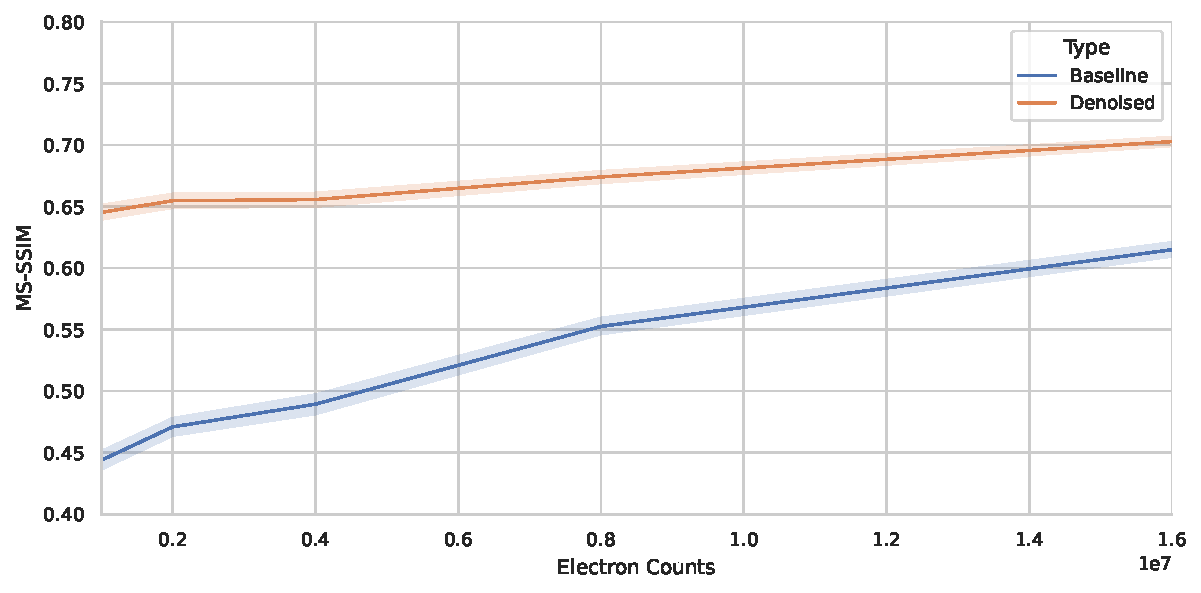
\includegraphics[width=1\linewidth]{images/nn_gdw_msssim.pdf}
    \caption{Denoising performance of (best) neural network as a function of \gls{ncounts}, measured using \gls{MSSSIM}. The comparison is done with slice-summed target with $w=10$. The baseline metric is computed using the noisy image as input. Different from \gls{BM3D}, the neural network denoising performance stays relatively consistent across the \gls{ncounts}, and is especially effective at lower counts.}
    \label{fig:gdw-test-metirc}
\end{figure}


At the end, we can look how the \gls{MSSSIM} scores improve with increasing counts, similar to how it is done with BM3D in \cref{fig:bm3d-msssim}. We have only looked at the best model but the same could be done for the last model. The \gls{MSSSIM} scores are shown in \cref{fig:gdw-test-metirc}, where the comparison is done between single slice denoised images with a slice summed target image ($w=10$). Perceptually (see \cref{fig:nn-denoised-counts-best-last-xy-bm3d-slice-sum-last-model}) the denoising performance with neural network far exceeds that of BM3D at low counts, even when denoising slice summed images with BM3D. The neural network denoising performance is also better than BM3D at higher counts for single slices, but the slice summed images and high counts ($geq \num{8e6}$) is just as good, or better. We do not discuss the \gls{MSSSIM} scores in detail, as the perceptual results are more important, and the \gls{MSSSIM} scores are consistent with the perceptual results.



% \begin{figure}
%     \centering
%     \begin{subfigure}[b]{1\linewidth}
%         \centering
%         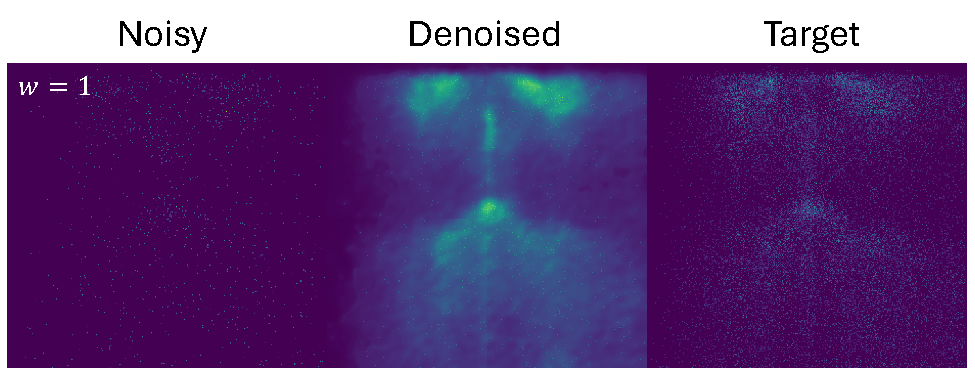
\includegraphics[width=1\linewidth]{images/nn_denoised_ex_w_1.pdf}
%         \caption{}
%         \label{fig:nn-denoised-ex-w-1}
%     \end{subfigure}

%     \begin{subfigure}[b]{1\linewidth}
%         \centering
%         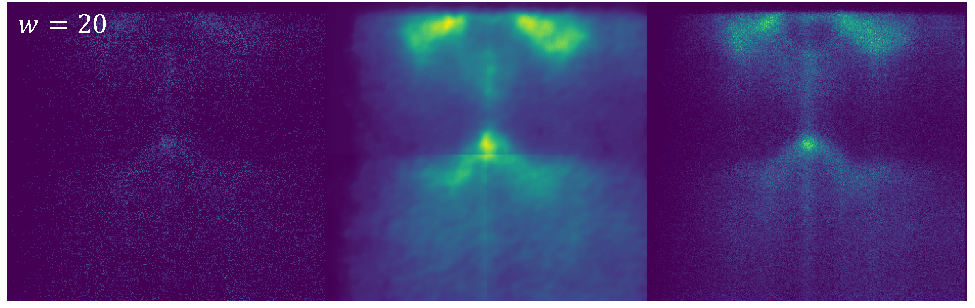
\includegraphics[width=1\linewidth]{images/nn_denoised_ex_w_20.pdf}
%         \caption{\num{4e6} count dataset. The denoising performance leaves room for improvement, using the adjusted optimal $\sigma_{\text{o}}\approx0.4$.}
%         \label{fig:nn-denoised-ex-w-20}
%     \end{subfigure}
%     \caption{}
%     \label{fig:nn-denoised-ex-w}
% \end{figure}

% \begin{figure}
%     \centering
%     \begin{subfigure}[b]{1\linewidth}
%         \centering
%         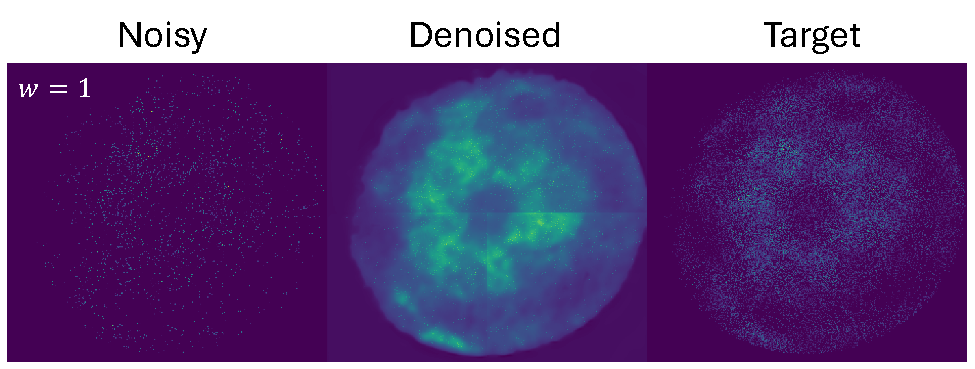
\includegraphics[width=1\linewidth]{images/nn_denoised_xy_w_1.pdf}
%         \caption{}
%         \label{fig:nn-denoised-xy-w-1}
%     \end{subfigure}

%     \begin{subfigure}[b]{1\linewidth}
%         \centering
%         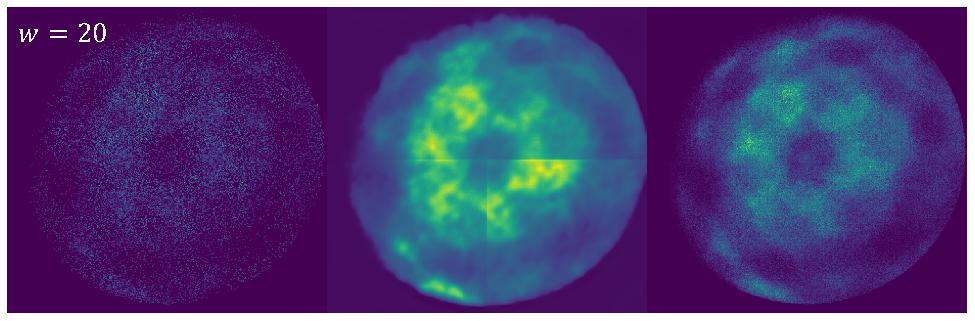
\includegraphics[width=1\linewidth]{images/nn_denoised_xy_w_20.pdf}
%         \caption{}
%         \label{fig:nn-denoised-xy-w-20}
%     \end{subfigure}
%     \caption{}
%     \label{fig:nn-denoised-xy-w}
% \end{figure}


% \begin{figure}[h]
%     \centering
%     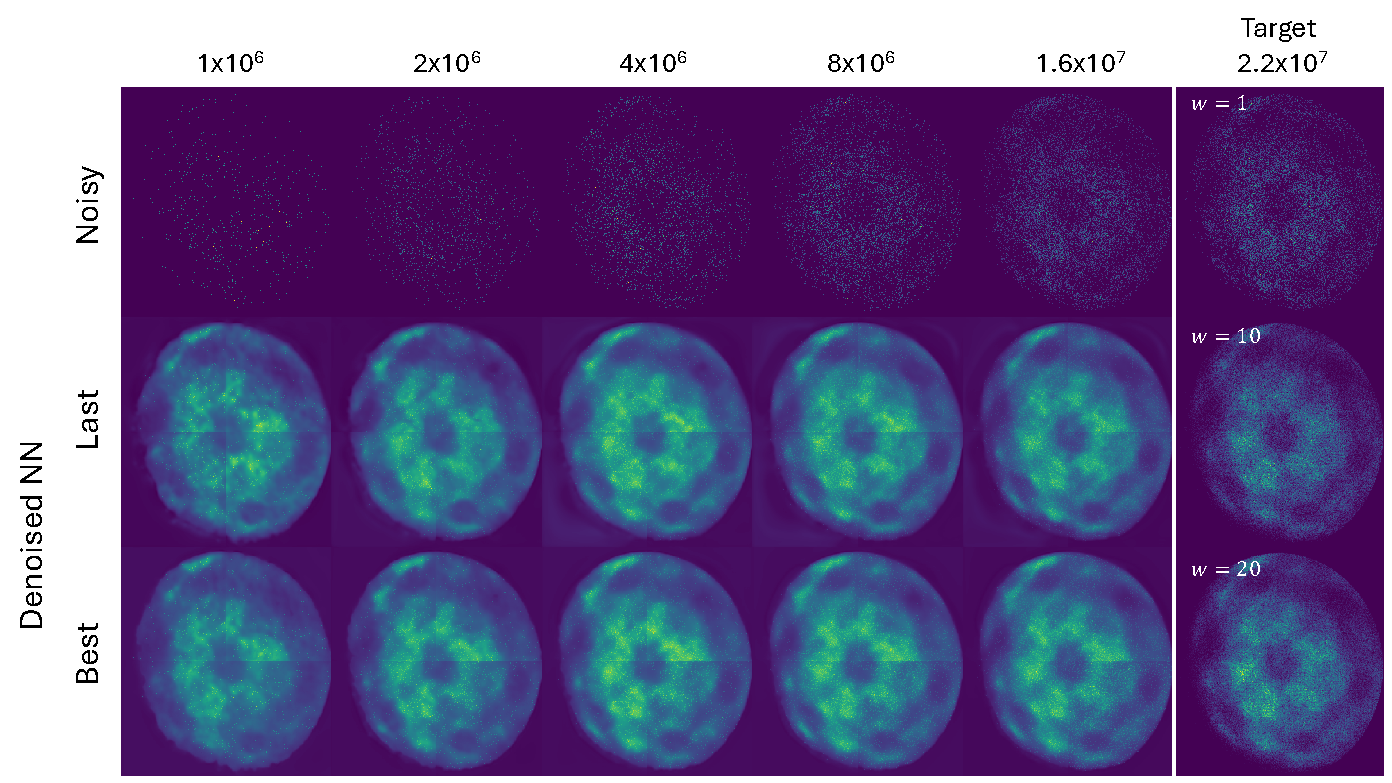
\includegraphics[width=1\linewidth]{images/nn_denoised_counts_best_last_xy.pdf}
%     \caption{}
%     \label{fig:nn-denoised-counts-best-last-xy}
% \end{figure}

% \begin{figure}[h]
%     \centering
%     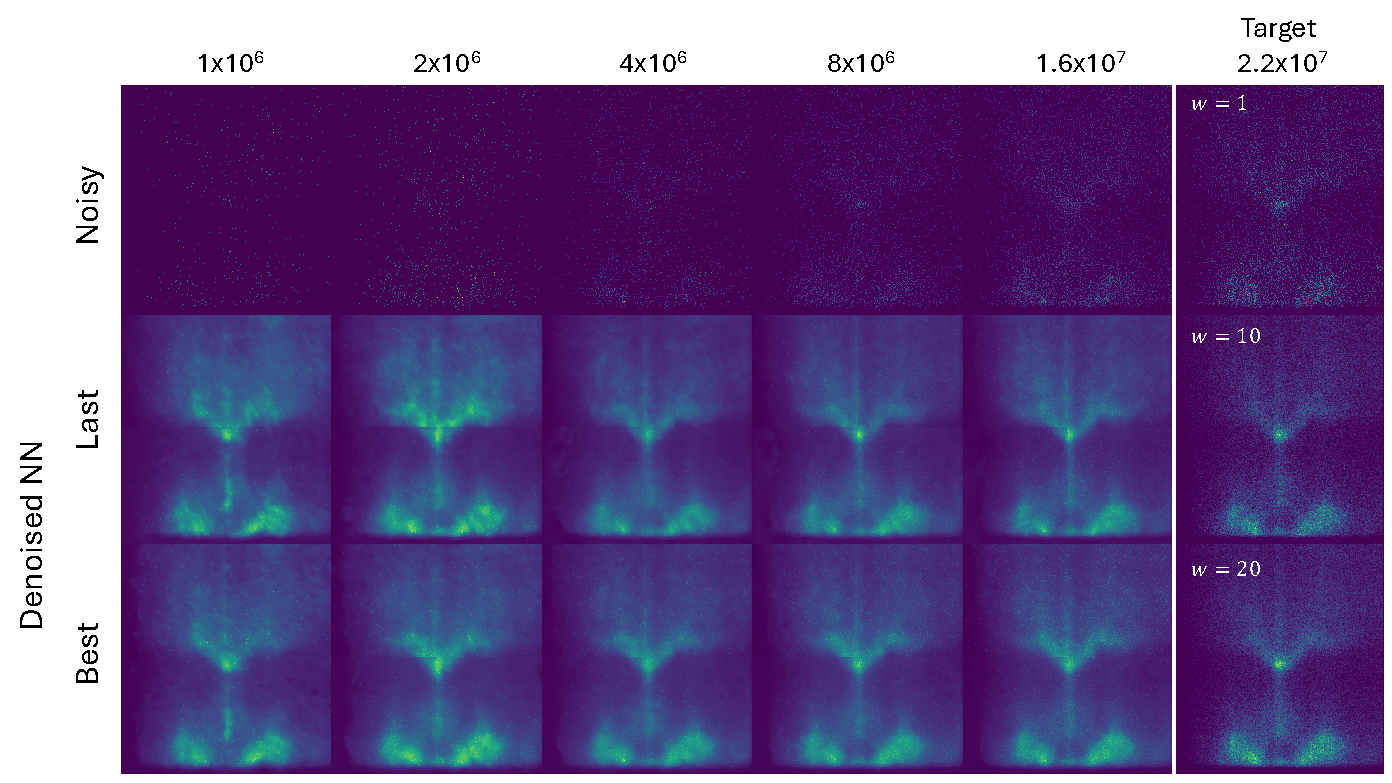
\includegraphics[width=1\linewidth]{images/nn_denoised_counts_best_last_ex.pdf}
%     \caption{}
%     \label{fig:nn-denoised-counts-best-last-ex}
% \end{figure}




\chapter{Conclusion and Outlook}
This thesis has presented an investigation into image denoising methodologies within the scope of \gls{MPES} data, addressing inherent limitations posed by the probabilistic nature of photoemission events, the multidimensional sample spaces, and compounded by the experimental constraints such as space-charge effect, sample degradation from radiation damage and practical constraints such as limited  beamtime allocations. These challenges are particularly pronounced in modern \gls{MPES} experiments leveraging cutting-edge light sources such as \glspl{FEL} and \gls{HHG} lasers that present unique statistical and operational challenges.

The work initially considered the \glsxtrfull{BM3D}, with and without variance stabilization through the Anscombe transform. While, these methods performed quite well for high-count data, the performance degrades considerably in the low-count regimes, reflecting their inability to exploit the multidimensional correlations intrinsic to the MPS data. While, perceptual improvements were observed with the Anscombe transform compared to just using \gls{BM3D}, the lack of clean target datasets rendered quantitative assessment of this effect challenging. We showed that \gls{MSSSIM} is a better metric with a noisy target, but more domain-specific evaluation metrics, tailored to the physics of \gls{MPES}, such as line shape analysis of momentum and energy distribution curves, could prove more beneficial.

This work has also contributes to the statistical analysis of photoemitted electrons, with an emphasis on electron counting distributions under FEL illumination. Our analysis confirmed that the stochastic SASE process is described by a doubly stochastic Poisson point process giving rise to NB counting statistics. The results presented here underscore the necessity of revising the commonly assumed Poisson model  within photoemission data and highlights the necessity of reevaluating models for variance stabilization and noise assessment in \gls{MPES}, especially when utilizing nonlinear \gls{HHG} sources or \glspl{FEL}. These insights, grounded in both theoretical analysis and experimental data, extend beyond \gls{MPES} to other disciplines reliant on similar photon-based counting experiments.

In order to overcome the constraints of traditional techniques within the extremely low-count regime, this thesis focused on deep learning methodologies, specifically the UNet3D architecture trained within the self-supervised learning paradigm, Noise2Noise. Exploiting the  correlations intrinsic to multidimensional data and using single-event datasets in order to create training examples, this model achieves  remarkable improvements in denoising in sparse \gls{MPES} datasets. We showed that for as little as \num{1e-3} average counts per voxel, the model predictions (corresponding to a \num{1e6} dataset) exceed higher count \gls{BM3D}-denoised images.

Advancements in variance stabilization techniques and their inversions for negative binomial noise, paired with an algorithm such as BM4D, leveraging 3D data, could prove useful when faced with no training data. The deep learning training would benefit from retraining using the \gls{MSSSIM} metric of evaluation and if possible, clean images. It would also be interesting to incorporate other experimental setup datasets, and also to try pretrained networks, or try unsupervised approaches such as Deep Image Prior and Noise2Void.

The potential impact of this work would enable more efficient data acquisition and analysis, the methods developed here streamlining experiments at large-scale facilities such as \glspl{FEL} or table-top laboratory setups, optimizing beamtime usage and expanding the scope of feasible studies. Furthermore, the insights into counting statistics and denoising techniques may be applicable to other counting experiments, such as x-ray diffraction, scattering, and other multidimensional spectroscopies. These methodologies also hold promise for applications in other fields facing difficulties with sparse, noisy datasets, such as medical imaging, astronomy, and particle physics.

Despite its successes, this work faced several limitations, including restricted test datasets and the lack of clean ground truths for metric evaluation. Addressing these limitations will be a priority for future studies, which could explore validation with domain-specific metrics, and expanded datasets encompassing a wider range of noise levels and experimental conditions. 

Beyond its methodological contributions, this thesis can serve as a valuable resource for experimental physicists and data scientists alike, providing detailed descriptions of the \gls{MPES} process, instrumentation, and theoretical foundations and discussion of deep learning.


% so this thesis has presented a comprehensive investigation into image denoising methodologies within the scope of, but not limited to MPES data. I presented  thorough introduction to the experimental technique, which is at the forefront of scientific avenue, but with challenges coming from the physical laws of nature; the probabilistic nature of pes. The inherent noise in light source, shot noise, is discussed. Difficulties due to  filling of multidimensional sample space, due to the space charge effect in \gls{trPES} are discussed to set the stage. limitations of beamtime allocations restricting the number of measurements that can be taken as well. 
% we talk about the complex segemented delay line detector that is used, and how this affects event counting and the data that is generated.

% specifically in \cref{ch:pes-statistics}, we dove deep into counting statistics of photoemitted electrons. We refer to extensive literature that contributed to the topic of photoelectron statistics and also show through our data that it follows the hypotheiszed results. Namely that the SASE process of FEL is following a doubly stochastic poisson point process and the counting statistics are negative binomial. The poisson assumption is valid only for coherent laser light sources, and not even for certain as the non-linear HHG process light sources (used in mpes actually) have recently been shown to have varying statistics by \citeauthor{gorlachQuantumopticalNatureHigh2020}. but these results are presented after an introduction to our experimental setup, which is used an FEL source. However, the findings here are not restrictive to this. Just interesting to note that one should be careful when assuming poisson statistics in their data.

% we have analyzed the usage of metrics, since we dont have clean targets to compare against. we decided to use \gls{MSSSIM} as it provided best distinction between noisy and denoised data but ideal situation for future work would be to have a clean target to compare against, or a more domain specific metric such as Line shape analysis, mdcs, commonly used derivative based techinque in arpes etc.
% But still using this metric, we show that the metric reports similar performance for both bm3d with and without variance stabilization through anscombe but perceptually, the anscombe leads to a bit more better results, due to the stabilization of variance, and hence not excessive denoising for high count data, compared to the lower count data.

% for future work, vsts for nb noise can be discussed but in this thesis we discussed results already published regarding vsts and optimal inverses of poisson noise as that is the common assumption, which we learnt to be false, though this is also in published research already about photoelectrons statistics by mandel in general and specifically by fel creators \citeauthor{saldinStatisticalPropertiesRadiation1998}

% lastly, key contribution in extremely low count statistics (talking an average voxel count of \num{1e-3} which correponds to a \num{1e6} dataset) is the use of deep learning, specifically unet3d, trained on noise2noise paradigm. this approach accesses the spatial correlations in the data and is able to denoise the data effectively. we do this training with limitless access to training data as we have access to event data that we can bin independent realizations from. this is a promising approach for future work, as it can be extended to other datasets and other denoising tasks.
% as mentioned before, we have limited data, and the test dataset we employed had max counts of \num{2.21e6}, which corresponds to about half that count in the image itself (since we filter some ranges out). this shows perceptually amazing results for extremely low counts but since we train on the lower counts, it doesn't perform as well on higher counts. moreover, a better validation set is needed to validate the model, and currently we used ssim (as this was done before) for metric but in future msssim as metric is planned. The effect of training set should also be investigated, as we used significant amount of data but this also requiers a very long training process. we should also inspect the effect of noise levels on the training process, as we used really high noise levels (very low counts as said). 

% A big contribution to describe everything that has been used is made, such as pes process, hhg, fel, momentum microscopes, such as the deep learning algorithms and it's basis from statistical learning paradigms so that this can be used as a reference for future work.

% the research has potential to streamline the MPES data acquisition process at table-top/laboratory sources as well as large-scale facilities like FEL FLASH. By utilizing our method in future studies, researchers will be able to efficiently optimize acquisition parameters; thus, significant beamtime could be conserved, or an existing beamtime budget could be used more effectively, allowing for the exploration of a broader parameter space.

% this work can also be used as a direction to others using fel facilities doing other counting experiments, such as x-ray diffraction, x-ray scattering, etc. as the counting statistics are similar, and the description we provided could aid in exploring this for such researchers. you can suggest other fields where such would be valuable.



% % Bibliography
% \bibliography{references}
\printbibliography[heading=bibintoc, title={Bibliography}]


% Additional chapters
% TODO: Add acknowledgements back
\chapter*{Acknowledgements}
\addcontentsline{toc}{chapter}{Acknowledgements}
This thesis would not have been possible without the constant support and guidance of the many people that supported me through the process. Though extremely challenging in the breath and depth I tried to uptake, it allowed me to explore many directions of research and allowed me to learn a lot, and for that I am thankful.

I would like to especially express my gratitude to my supervisors B. Berkels and Kai, and Dima, my acting supervisor throughout the thesis. I am very thankful to B. Berkels for accepting to supervise this external research project. I appreciate the commitment made to constantly guide me in the right direction, especially in the fields of image denoising and mathematics relating. I am thankful to Kai for the detailed discussions on exploring different physics, and supporting me in presenting my research. I would especially like to thank Dima for the consistent guidance throughout this project, for helping me understand all the details surrounding the experimental aspects of MPES, and for always being very understanding.

Naturally, no work is complete without the help of those close and dear. I extend my heartfelt thanks to the closest for the consistent support through the fun and the tough times. Shoutout to Kumarah who stayed up late nights helping me with corrections, in a domain he had little clue of.

I also extend my gratitude to Martin Burger's group. Especially to Lorenz Kruger for the insightful conversations trying to explore the data, its statistical implications and more.

This contribution was made possible through the generosity of the authors who shared their datasets: groups from DESY/FLASH, University of Mainz, FU Berlin, ETH Zürich for the \gls{GdW} dataset \cite{kutnyakhovMultidimensionalPhotoemissionSpectra2024}, \citeauthor{heberMultispectralTimeresolvedEnergy2022} and groups from ETH Zürich, DESY/NanoLab and Aarhus University for the \gls{GrIr} dataset \cite{heberMultispectralTimeresolvedEnergy2022}, and \citeauthor{maklarTimeresolvedARPESRAW2022} for the \gls{WSe2} dataset \cite{maklarTimeresolvedARPESRAW2022}.

We acknowledge DESY (Hamburg, Germany), a member of the Helmholtz Association HGF, for the provision of experimental facilities. Parts of this research were carried out at PG2 beamline of FLASH. This research was also supported in part through the Maxwell computational resources operated at DESY, Hamburg, Germany.

The \texttt{Python} data science and visualization ecosystem was heavily employed in this thesis.
The usage of \texttt{Xarray} \cite{hoyerXarrayNDLabeled2017} for multidimensional dataset transformations, \texttt{matplotlib} \cite{hunterMatplotlib2DGraphics2007} for plotting of images and other figures, \texttt{pandas} \cite{thepandasdevelopmentteamPandasdevPandasPandas2024} for tabular assessment of data, \texttt{seaborn} \cite{waskomSeabornStatisticalData2021} for statistical plotting, \texttt{optuna} \cite{akibaOptunaNextgenerationHyperparameter2019} for hyperparameter optimization, are acknowledged by citation as this is preferred by these scientific libraries. 

Extensive use of the \texttt{SED} (\href{https://github.com/OpenCOMPES/sed}{https://github.com/OpenCOMPES/sed}) is made, especially allowing easy manipulation of the single-event dataframes with $>$\num{1e9} rows, extremely fast binning to multidimensional images and compatibility with HDF5 and tiff formats.

For deep learning, exclusively \texttt{PyTorch} \cite{paszkePyTorchImperativeStyle2019} has been used. We use the \texttt{UNET3D} shown in \cite{cicek3DUNetLearning2016}, implemented (modified to accommodate our needs) by \citeauthor{wolnyAccurateVersatile3D2020} \cite{wolnyAccurateVersatile3D2020}. \texttt{PyTorch} \texttt{Dataset} and \texttt{DataLoader} classes were extensively used to ease in experiments other than deep learning.

Many of the concepts about Statistical Learning Theory were introduced to the author by the lecture series \textit{Algorithmic Foundations of Data Science} taught by Prof. M Grohe at the RWTH Aachen University. And much of their mathematical understanding on signal and image processing is based on the lecture series \textit{Mathematical Methods of Signal and Image processing} taught by Prof. B Berkels.


\chapter*{Contributions}
\addcontentsline{toc}{chapter}{Contributions}
A preliminary analysis during the early works of this thesis titled
\textit{Efficient Data Acquisition in Multi-Dimensional Photoemission Spectroscopy using Denoising}, was presented, in the form a of poster, at the DPG Spring Meetings 2024, as well as NanoMat Science Day 2024 at DESY. 


% \chapter*{Declaration}
% \addcontentsline{toc}{chapter}{Declaration}
% Insert declaration here
\vspace*{\fill}
Date \& Signature: \hrulefill


% \printindex

\clearpage
\pagenumbering{Roman}

\begin{appendices}
  \chapter{Mathematical Background}
\label{appendix:mathematical-notation}

\section{Law of Large Numbers}\label{section:law-of-large-numbers}
Consider a sequence of \gls{iid} random variables $X_1, X_2, \dots, X_n$ defined on the probability space $(\Omega, \mathcal{A}, P)$ (see \cref{section:probability-notation}), representing the number of detected events in different intervals. Since the random variable are \gls{iid}, the expected value $\mu$ of each $X_i$ is the same. The true mean (or expected value) of these random variables can be defined as $\mu = \mathbb{E}(X_1)$, and the variance as $\sigma^2 = Var(X_1)$.

Formally, by the law of large numbers\footnote{Specifically, the weak law of large numbers, which also has a stronger variant proving almost surely (a.s.) convergence.}, the sample mean $\bar{X_n} = \frac{1}{n} \sum_{i=1}^{n} X_i$ converges in probability to the expected value $\mu$ as $n \to \infty$ \cite{fellerIntroductionProbabilityTheory1991a}:
\begin{equation}
    \lim_{n \to \infty} P(|\bar{X_n} - \mu| > \epsilon) = 0
\end{equation}

The rate of convergence to $\bar{X_n}$ is of practical importance, as it indicates how quickly the sample statistics approximate the true distribution:
\begin{equation}
    \left|\bar{X_n} - \mu\right| = \mathcal{O}\left(\frac{1}{\sqrt{n}}\right)
\end{equation}

indicating that the relative fluctuations decrease with an increased number of observations \gls{ncounts}.  Increasing the acquisition time $T$ reduces the sample mean fluctuations, since $n \propto T$. While convergence rate described by $\mathcal{O}\left(\frac{1}{\sqrt{n}}\right)$ is a fundamental result, the constant that accompanies this rate is distribution dependent, and can affect the convergence rate. The Big O notation, denoted as $\mathcal{O}(g(n))$, describes an upper bound on the time complexity of an algorithm or the growth rate of a function.

\section{Measure Space and Measures}
\label{section:measurable_space}
\begin{note}
    {Measurable Space}

    Let $\Omega = \emptyset$, $P(\Omega)$ the power set of $\Omega$ and $\mathcal{A} \subset P(\Omega)$. If the following conditions are met, $\mathcal{A}$ is a called $\sigma$-algebra, and the $(\Omega, \mathcal{A})$ pair make up a measurable space.
    \begin{enumerate}
        \item $\Omega \in \mathcal{A}$.
        \item If $A \in \mathcal{A}$, then $\Omega \setminus A \in \mathcal{A}$.
        \item If $(A_n)_{n \in \mathbb{N}}$ is a sequence of sets where $A_n \in \mathcal{A}$ for all $n \in \mathbb{N}$, then 
        \begin{equation*}
            \bigcup_{n \in \mathbb{N}} A_n \in \mathcal{A}.
        \end{equation*}
    \end{enumerate}
\end{note}

\begin{note}
    {Positive Measure}
    Let $(\Omega, \mathcal{A})$ be a measurable space as defined in above. A function $\mu: \mathcal{A} \to [0, \infty]$ is called a \textit{positive measure} if it satisfies the following conditions:

    \begin{enumerate}
        \item $\mu(\emptyset) = 0$, (the measure of the empty set is zero)
        \item $\mu$ is \textit{countably additive}: For any countable collection of disjoint sets $(A_i)_{i \in \mathbb{N}} \subset \mathcal{A}$, we have
        \begin{equation*}
            \mu\left( \bigcup_{i=1}^{\infty} A_i \right) = \sum_{i=1}^{\infty} \mu(A_i).
        \end{equation*}
    \end{enumerate}
    
    If these conditions are met, then $\mu$ is called a \textit{measure} on the measurable space $(\Omega, \mathcal{A})$, and the triple $(\Omega, \mathcal{A}, \mu)$ is called a \textit{measure space}.
\end{note}



\section{Probability}\label{section:probability-notation}
The theory of probability is necessary to quantify stochastic and uncertain quantities. Throughout this text, it can be seen used the in context of inherently stochastic processes, such as quantum effects, and to quantify uncertainty in measurements.

\begin{note}
    {Probability Measure}
A \textit{probability measure} $P: \mathcal{A} \to [0, 1]$ satisfies all the properties of a positive measure (see Section \ref{section:measurable_space}), with the additional property known as the normalization condition:

\begin{equation*}
    P(\Omega) = 1
\end{equation*}

This leads to the measure space for probability (or probability space) being $(\Omega, \mathcal{A}, P)$. The probability of an event $A \in \mathcal{A}$ is $P(A)$. The probability measure is hence a real number between 0 and 1 that defines the likelihood of an event to occur.
\end{note}

% In the \textit{frequentist} interpretation, probability is defined as the long-run relative frequency of an event occurring in repeated independent trials. It assumes that probabilities are objective and intrinsic properties of the physical world. For example, the probability of getting heads in a fair coin toss is 0.5, meaning that if we were to toss the coin an infinite number of times, half of the outcomes would be heads.

% The \textit{Bayesian} interpretation, on the other hand, views probability as a measure of belief or certainty about an event, given the available information. It is inherently subjective and updates as new evidence is introduced. For instance, if we initially believe that a coin is fair, but after observing several tosses we notice a bias, we update our belief (and hence the probability) to reflect the new evidence. This process of updating beliefs is formalized through \textit{Bayes' rule}, which is a cornerstone of Bayesian inference.

% \begin{note}{Law of Total Probability}
%     The law of total probability provides a way to compute the probability of an event based on a partition of the sample space. If $\{B_i\}_{i=1}^{n}$ is a partition of the sample space $\Omega$ (i.e., $B_i \cap B_j = \emptyset$ for $i \neq j$ and $\bigcup_{i=1}^{n} B_i = \Omega$), then for any event $A$:

%     \begin{equation}
%         P(A) = \sum_{i=1}^{n} P(A \mid B_i) P(B_i).
%     \end{equation}
    
%     This law is particularly useful when dealing with complex events that can be decomposed into simpler, mutually exclusive cases.
    
% \end{note}

\subsection{Distributions}
\begin{note}
    {Poisson distribution}\label{note:poisson-distribution}
    The \gls{PMF} for Poisson distribution Poi\((\lambda)\) with \(\lambda > 0\) is defined as
    \begin{equation}\label{eq:poisson-pmf}
        P(n;\lambda) = \frac{\lambda^n e^{-\lambda}}{n!}, \quad n \in \mathbb{N}_0
    \end{equation}
    \begin{enumerate}
        \item $\lambda = E(X) = Var(X)$ 
        \item Additivity: If $X_1 \sim \text{Poi}(\lambda_1)$ and $X_2 \sim \text{Poi}(\lambda_2)$ are independent Poisson random variables, then the sum $X_1 + X_2$ also follows a Poisson distribution with parameter $\lambda_1 + \lambda_2$
        \begin{equation}
            X_1 + X_2 \sim \text{Poi}(\lambda_1 + \lambda_2).
        \end{equation}
        
        This property is useful when considering counts from multiple independent sources.
    \end{enumerate}
\end{note}

For overdispersed count data, the \gls{NB} is suitable. 

\begin{note}
    {Negative Binomial Distribution}\label{note:negative-binomial-distribution}
    The \gls{PMF} for the \gls{NB} distribution, denoted $\text{NB}(r, p)$, where:
    \begin{itemize}
        \item $r > 0$ is the number of successes,
        \item $p \in (0, 1)$ is the probability of success on each trial,
    \end{itemize}
    is defined as:
    \begin{equation}\label{eq:nb-pmf}
        P(k; r, p) = \binom{k+r-1}{r-1} (1-p)^k p^r, \quad k \in \mathbb{N}_0
    \end{equation}
    where $k$ is the number of failures that occur before the $r$-th success.
    For $X \sim \text{NB}(r, p)$, the mean is given by:
        \begin{equation}
            E(X) = \frac{r(1-p)}{p}
        \end{equation}
        and the variance is:
        \begin{equation}
            Var(X) = \frac{r(1-p)}{p^2}
        \end{equation}

\end{note}


For relation between Poisson, \gls{NB} and Gamma distributions, see \cite{barry2020gamma}. It can be shown that \gls{NB} converges to Poisson as $r \to \infty$. The \gls{NB} distribution can also be considered as a mixture of Poisson distributions with a Gamma prior on the rate parameter $\lambda$.

% \subsection{Central Limit Theorem}
% % Central Limit Theorem (CLT)
% Consider again a sequence of \gls{iid} random variables $X_1, X_2, \dots, X_n$ defined on the probability space $(\Omega, \mathcal{A}, P)$. The Central Limit Theorem states that for such an \gls{iid} sequence with mean $\mu$ and variance $\sigma^2$, the normalized sum of these variables converges in distribution to the standard normal distribution as $n$ tends to infinity:

% \begin{equation}
%     \frac{\sum_{i=1}^{n} X_i - n\mu}{\sigma \sqrt{n}} \xrightarrow{d} \mathcal{N}(0, 1) \quad \text{as} \quad n \to \infty.
% \end{equation}

% \begin{note}{Conditional Probability}
%     Conditional probability quantifies the probability of an event occurring given that another event has already occurred. If $A$ and $B$ are two events in a probability space with $P(B) > 0$, the \textit{conditional probability} of $A$ given $B$ is defined as:
    
%     \begin{equation}
%         P(A \mid B) = \frac{P(A \cap B)}{P(B)}.
%     \end{equation}
%     This measure allows us to update the likelihood of an event based on new information provided by the occurrence of another event.
%     \end{note}
    
%     \begin{note}{Marginal Probability}
%     Marginal probability, also known as the \textit{unconditional probability}, refers to the probability of an event irrespective of the outcomes of other variables. If $A$ is an event in a probability space, the marginal probability of $A$ is simply $P(A)$. 
    
%     For discrete random variables $X$ and $Y$, the marginal probability of $X$ can be found by summing the joint probabilities over all values of $Y$:
    
%     \begin{equation}
%         P(X = x) = \sum_{y} P(X = x, Y = y).
%     \end{equation}
    
%     Similarly, for continuous random variables, the marginal probability density function is obtained by integrating the joint probability density function over all possible values of the other variables.
    
%     \end{note}

    
% Another interpretation:
% \begin{note}{Bayes' Rule}
% Bayes' rule is a fundamental theorem in probability theory that relates conditional and marginal probabilities. Given two events $A$ and $B$ with $P(B) > 0$, Bayes' rule states:

% \begin{equation}
%     P(A \mid B) = \frac{P(B \mid A) P(A)}{P(B)}.
% \end{equation}

% Bayes' rule allows us to update our beliefs about the probability of event $A$ occurring based on new evidence represented by event $B$. It forms the backbone of Bayesian inference, where prior beliefs are updated with new data.

% \end{note}

% \begin{note}{Application of Bayes' Rule}
%     Bayes' rule can be extended using the law of total probability:
    
%     \begin{equation}
%         P(A \mid B) = \frac{P(B \mid A) P(A)}{\sum_{i} P(B \mid A_i) P(A_i)},
%     \end{equation}
    
%     where $\{A_i\}$ is a partition of the sample space. This formula is useful in scenarios involving multiple hypotheses or models.
% \end{note}

% \section{Landau Notation}
% Landau notation, commonly referred to as Big O notation and its relatives (Big Omega, Big Theta, etc.), is used to describe the asymptotic behavior of functions. This is particularly important in the analysis of algorithms and in expressing the growth rates of functions.

% \section*{Big O Notation ($\mathcal{O}$)}
% Big O notation, denoted as $\mathcal{O}(g(n))$, describes an upper bound on the time complexity of an algorithm or the growth rate of a function. It provides an asymptotic upper bound on the function.

% % \begin{equation}
% % f(n) = O(g(n)) \quad \text{if and only if there exist positive constants } C \text{ and } n_0 \text{ such that for all } n \geq n_0, \; |f(n)| \leq C \cdot |g(n)|.
% % \end{equation}

% \section*{Big Omega Notation ($\Omega$)}
% Big Omega notation, denoted as $\Omega(g(n))$, describes a lower bound on the time complexity or growth rate of a function. It provides an asymptotic lower bound.

% % \begin{equation}
% % f(n) = \Omega(g(n)) \quad \text{if and only if there exist positive constants } C \text{ and } n_0 \text{ such that for all } n \geq n_0, \; |f(n)| \geq C \cdot |g(n)|.
% % \end{equation}

% \section*{Big Theta Notation}
% Big Theta notation, denoted as $\Theta(g(n))$, provides both an upper and lower bound on the growth rate of a function. It effectively means that $(f(n)$) grows asymptotically at the same rate as $(g(n)$).

% % \begin{equation}
% % f(n) = \Theta(g(n)) \quad \text{if and only if there exist positive constants } C_1, C_2 \text{ and } n_0 \text{ such that for all } n \geq n_0, \; C_1 \cdot |g(n)| \leq |f(n)| \leq C_2 \cdot |g(n)|.
% % \end{equation}

% \section*{Little o Notation}
% Little o notation, denoted as \(o(g(n))\), describes an upper bound that is not asymptotically tight. In other words, \(f(n)\) grows strictly slower than \(g(n)\).

% % \begin{equation}
% % f(n) = o(g(n)) \quad \text{if and only if \(\lim_{n \to \infty} \frac{f(n)}{g(n)} = 0\).
% % \end{equation}

% \section*{Little Omega Notation}
% Little omega notation, denoted as $\omega(g(n))$, describes a lower bound that is not asymptotically tight. This means that \(f(n)\) grows strictly faster than $(g(n)$).

% % \begin{equation}
% % f(n) = \omega(g(n)) \quad \text{if and only if \(\lim_{n \to \infty} \frac{f(n)}{g(n)} = \infty\).
% % \end{equation}

% \section*{Usage in Analysis}
% Landau notation is extensively used in algorithm analysis to describe the running time or space requirements of an algorithm as a function of the input size. It abstracts away constants and less significant terms, focusing on the dominant factor that impacts growth rate as input size increases.


\section{Statistical Inference}
% For goodness-of-fit tests, small $p$-values indicate that you can reject the null hypothesis and conclude that your data were not drawn from a population with the specified distribution. In the case of such tests, a high $p$-value would suggest that the observed data and the expected distribution are statistically similar.
% \subsection*{Goodness of Fit Tests}\label{section:chi-test}
% We hypothesize that the data follows a certain distribution based on theoretical grounding and visualize analysis. Specifically, that data from a laser follows a Poisson distribution and from an \gls{FEL} a \gls{NB} distribution. One possible way to test these hypotheses is through a statistical test such as the Chi-Square Goodness of Fit test.

% The Chi-Square test determines if the observed frequencies of data fit with the expected frequencies derived from the hypothesized distribution. This test is particularly suitable for discrete data, making it appropriate for count data that follows Poisson or Negative Binomial distributions.

% \begin{note}
%     {Chi-Square Test}
%     Let  $O_i$  be the observed frequency in category  $i$ , and  $E_i$  be the expected frequency in category  $i$  under the hypothesized distribution. The Chi-Square test statistic  $\chi^2 $ is given by:
%     \begin{equation}
%         \chi^2 = \sum_{i=1}^k \frac{(O_i - E_i)^2}{E_i}
%     \end{equation}
%     where $k$ is the number of categories. The degrees of freedom for this test is given by:

%     The null hypothesis $H_0$ states that the observed data follows the specified distribution, while the alternative hypothesis $H_1$ posits that the observed data does not follow the specified distribution:

%     \begin{equation*}
%         H_0: \text{The data follows the specified distribution}
%     \end{equation*}
%     \begin{equation*}
%         H_1: \text{The data does not follow the specified distribution}
%     \end{equation*}
% \end{note}

% The Poisson dispersion test specifically examines whether the variance of the observed data significantly differs from the mean, as expected for a Poisson distribution, where the mean and variance should be equal. Deviations from this relationship may indicate overdispersion or underdispersion, which can inform the choice of an appropriate statistical model.
% \begin{note}
%     {Poisson Dispersion Test}
%     Let $O_i$ be the observed frequency in category $i$ and let $\lambda$ be the estimated mean of the observed data. The test statistic for the Poisson dispersion test is defined as:
%     \begin{equation}
%     D = \frac{S^2}{\bar{X}}
%     \end{equation}
%     where $S^2$ is the sample variance of the observed data and $\bar{X}$ is the mean of the observed counts.
%     Under the null hypothesis $H_0$ (the data follows a Poisson distribution), the test statistic $D$ follows a Chi-Square distribution with $n - 1$ degrees of freedom, where $n$ is the number of observed categories. 

% The null hypothesis and alternative hypothesis are stated as follows:

% \begin{equation*}
%     H_0: \text{The data follows a Poisson distribution}
% \end{equation*}
% \begin{equation*}
%     H_1: \text{The data does not follow a Poisson distribution}
% \end{equation*}
% \end{note}


\subsection{Confidence Intervals}
Confidence Intervals are a way to quantify the uncertainty in an estimate. They provide a range of plausible values for a parameter, rather than a single point estimate. The confidence level indicates the probability that the interval contains the true parameter value. For example, a 95\% confidence interval means that if we were to repeat the experiment many times, 95\% of the intervals would contain the true parameter value.

Parametric methods for computing confidence intervals rely on knowing the underlying distribution of the data, such as the normal distribution. However, in many cases, the true distribution is unknown or does not follow a standard form. In such cases, non-parametric methods such as bootstrapping can be used.

Bootstrapping involves resampling the data with replacement to create multiple bootstrap samples, from which the sample statistic is computed. The distribution of the sample statistic across the bootstrap samples provides an estimate of the sampling distribution of the statistic, and becomes more informative when using larger sample sizes.

% \subsection*{Optimal parameter estimation}
% Used in estimating distribution parameters

\section{Metrics}\label{sec:metrics}

\Gls{MSE} is a common measure of the average squared differences between predicted values and actual values. It quantifies the error in a model’s predictions, where lower values indicate better performance. It is sensitive to outliers since squaring the differences amplifies larger errors.

\begin{note}
    {\Glsxtrfull{MSE}}
    \begin{equation}\label{eq:mse}
        \text{MSE} = \frac{1}{N} \sum_{i=1}^{N} (x_i - y_i)^2
    \end{equation}
    \begin{itemize}
        \item $x_i$: pixel value of the noisy image
        \item $y_i$: pixel value of the target image
        \item $N$: total number of pixels
    \end{itemize}
\end{note}

\Gls{PSNR} is a measure of the peak error between two images, often used to evaluate image compression quality. It expresses the ratio between the maximum possible power of a signal and the power of corrupting noise. Higher PSNR values indicate better quality.

\begin{note}
    {\Glsxtrfull{PSNR}}
    \begin{equation}    
        \text{PSNR} = 10 \log_{10} \left( \frac{L^2}{\text{MSE}} \right)
    \end{equation}
    \begin{itemize}
        \item $L$: maximum pixel value of the image
        \item \gls{MSE}: mean squared error
    \end{itemize}
\end{note}


\Gls{SSIM} is a perceptual metric that quantifies the visual impact of three characteristics of an image: luminance, contrast, and structure. It evaluates the similarity between two images based on their structural information, making it more aligned with human visual perception than MSE or PSNR. Values range from -1 to 1, with 1 indicating perfect similarity.
\begin{note}
    {\Glsxtrfull{SSIM}}
    \begin{equation}    
        \text{SSIM}(x, y) = \frac{(2\mu_x \mu_y + C_1)(2\sigma_{xy} + C_2)}{(\mu_x^2 + \mu_y^2 + C_1)(\sigma_x^2 + \sigma_y^2 + C_2)}
    \end{equation}
    \begin{itemize}
        \item $\mu_x, \mu_y$: mean of $x$ and $y$
        \item $\sigma_x, \sigma_y$: standard deviation of $x$ and $y$
        \item $\sigma_{xy}$: covariance of $x$ and $y$
        \item $C_1 = (k_1L)^2, C_2 = (k_2L)^2$: constants to stabilize the division
    \end{itemize}
\end{note}

\Gls{MSSSIM} extends \gls{SSIM} by evaluating image similarity across multiple scales and resolutions. By considering different image scales, it captures more information about structural variations and perceptual quality, making it particularly useful for assessing image quality in applications like compression. Similar to \gls{SSIM}, higher values indicate greater similarity.

\begin{note}
    {\Glsxtrfull{MSSSIM}}
    \begin{equation}\label{eq:msssim}    
        \text{MSSSIM}(x, y) = \prod_{j=1}^{J} \text{SSIM}(x_j, y_j)^{\alpha_j}
    \end{equation}
    \begin{itemize}
        \item $J$: number of scales
        \item $x_j, y_j$: images at scale $j$
        \item $\alpha_j$: weight for scale $j$, summing to 1
    \end{itemize}
\end{note}

The metric implementations used in this thesis are either \texttt{PIQA} library \href{https://github.com/francois-rozet/piqa}{https://github.com/francois-rozet/piqa}, or \texttt{skimage} library \href{https://scikit-image.org/}{https://scikit-image.org/}.

  \chapter{Supplementary Material}
\section{Transforming Raw Data to structured format: Extract, Load, Transform}\label{sec:elt}
Raw data from the experiment is stored in \gls{HDF5} files. This includes many \gls{beamline} diagnostic information such as \gls{BAM}, \gls{GMD}, the delay stage readings, the monochromator energy, sample specific information such as extractor voltage, and the electron counting in the 3 detector dimensions corresponding to the \gls{DLD} spatial X and Y axes and the temporal time axis. This information is resolved at each bunch of electrons coming from the accelerator called a \gls{train}, which are further microbunched into \glsplural{pulse}.

The \gls{OpenCOMPES} was established to develop tools and infrastructure to make analysis easier. To this end, a modular Python library called \texttt{\gls{SED}} was created that provides the entire pipeline from easy data loading to common calibration and corrections, multidimensional binning to create images, and saving the images to standard formats, with proper care of data provenance.

The data pipeline follows an \gls{ELT} process, wherein raw data is extracted from \gls{HDF5} files, transformed into a structured format suitable for analysis, and subsequently stored in intermediate buffer files for further downstream processes such as analysis and visualization.

The following sections provide a detailed exposition of each stage of this \gls{ELT} process, also shown in \cref{fig:elt}. The first stage, extraction, begins with the loading of raw data from the \gls{HDF5} files. These files encapsulate experimental results across multiple channels, including electron-resolved and time-resolved data. The hierarchical structure of the \gls{HDF5} files allows the organization of data into groups, where each group contains an index and its corresponding dataset, collectively referred to as a “channel” The paths to these \gls{HDF5} files, along with relevant configuration parameters, are provided to the pipeline to dictate the steps of the subsequent transformation process.

\subsection*{Pipeline Overview}
To optimize performance and facilitate data management, the pipeline generates buffer files for each type of data (electron and time-resolved). This task is handled by the \texttt{BufferFilePaths} class, which initializes file paths and manages the creation of buffer files in the efficient \texttt{Parquet} format. By checking the presence of pre-existing buffer files, the class determines whether to reuse these files or regenerate them, based on the \texttt{force\_recreate} flag.

Each \gls{HDF5} file results in the generation of two primary buffer files: one containing electron-resolved data and another containing pulse/train-resolved data. These files are essential for organizing the data at the pulse level and maintaining resolution at the electron level. The data for each train contains roughly 500 pulses, and although some data is resolved at the pulse level, each index often holds an array, necessitating the use of the \texttt{pandas} MultiIndex functionality to maintain the data’s hierarchical structure. Detector measurements, which are electron-resolved along the X, Y, and temporal axes, are typically represented as three-dimensional arrays and add further complexity to the indexing process.

A critical transformation step involves correcting for offsets in pulse IDs to ensure accurate synchronization of data across different channels. Any data associated with pulse IDs below zero is removed, as it is considered invalid. Similarly, \texttt{NaN} pulses are dropped to avoid introducing inconsistencies in downstream analyses. While it is possible that pulses exceeding 500 may also be invalid, these are not filtered during this stage, as that determination is deferred to the final analysis. Due to machine fluctuations, pulses may become unsorted, and hence the pulses are sorted within each train to maintain temporal order.

Once this cleaning process is completed, electron-resolved channels are combined using an outer join with pulse and train-resolved channels, forming a comprehensive dataframe that contains all relevant information for further analysis. This merged dataset is separated into two primary dataframes: the electron-resolved dataframe and the pulse-resolved dataframe.

The electron dataframe contains only rows where electron events have been detected, with any missing data in non-electron channels forward-filled to ensure completeness. This dataframe serves as the main source of electron-specific data for further analyses. However, given that not all pulses or trains may produce electron events, a separate pulse-resolved dataframe is generated to capture all available train and pulse data, independent of electron detections. This pulse-resolved dataframe is essential for normalization steps involving time-resolved channels, such as those related to the delay axis.

The pipeline also includes validation steps for auxiliary channels, particularly those containing multidimensional data (e.g., 4D arrays), ensuring that all required channels exist within the files before proceeding with further transformations.

After this initial transformation and extraction, the buffer files are saved in \texttt{Parquet} format, chosen for its efficiency in storage and speed of access during future computations. The final stage involves the loading of all these buffer files into a unified dataframe using \texttt{Dask}, a distributed computing library that enables scalable processing of large datasets. At this stage, forward-filling is again applied to non-electron channels, ensuring that missing values between files are handled consistently. However, care must be taken when forward-filling across different runs, as this could introduce inter-run inconsistencies.

Finally, the schema of the buffer files is cross-validated against the predefined list of channels to ensure consistency and completeness prior to loading the data into \texttt{Dask}.

\begin{figure}[H]
    \label{fig:elt}
    \centering
    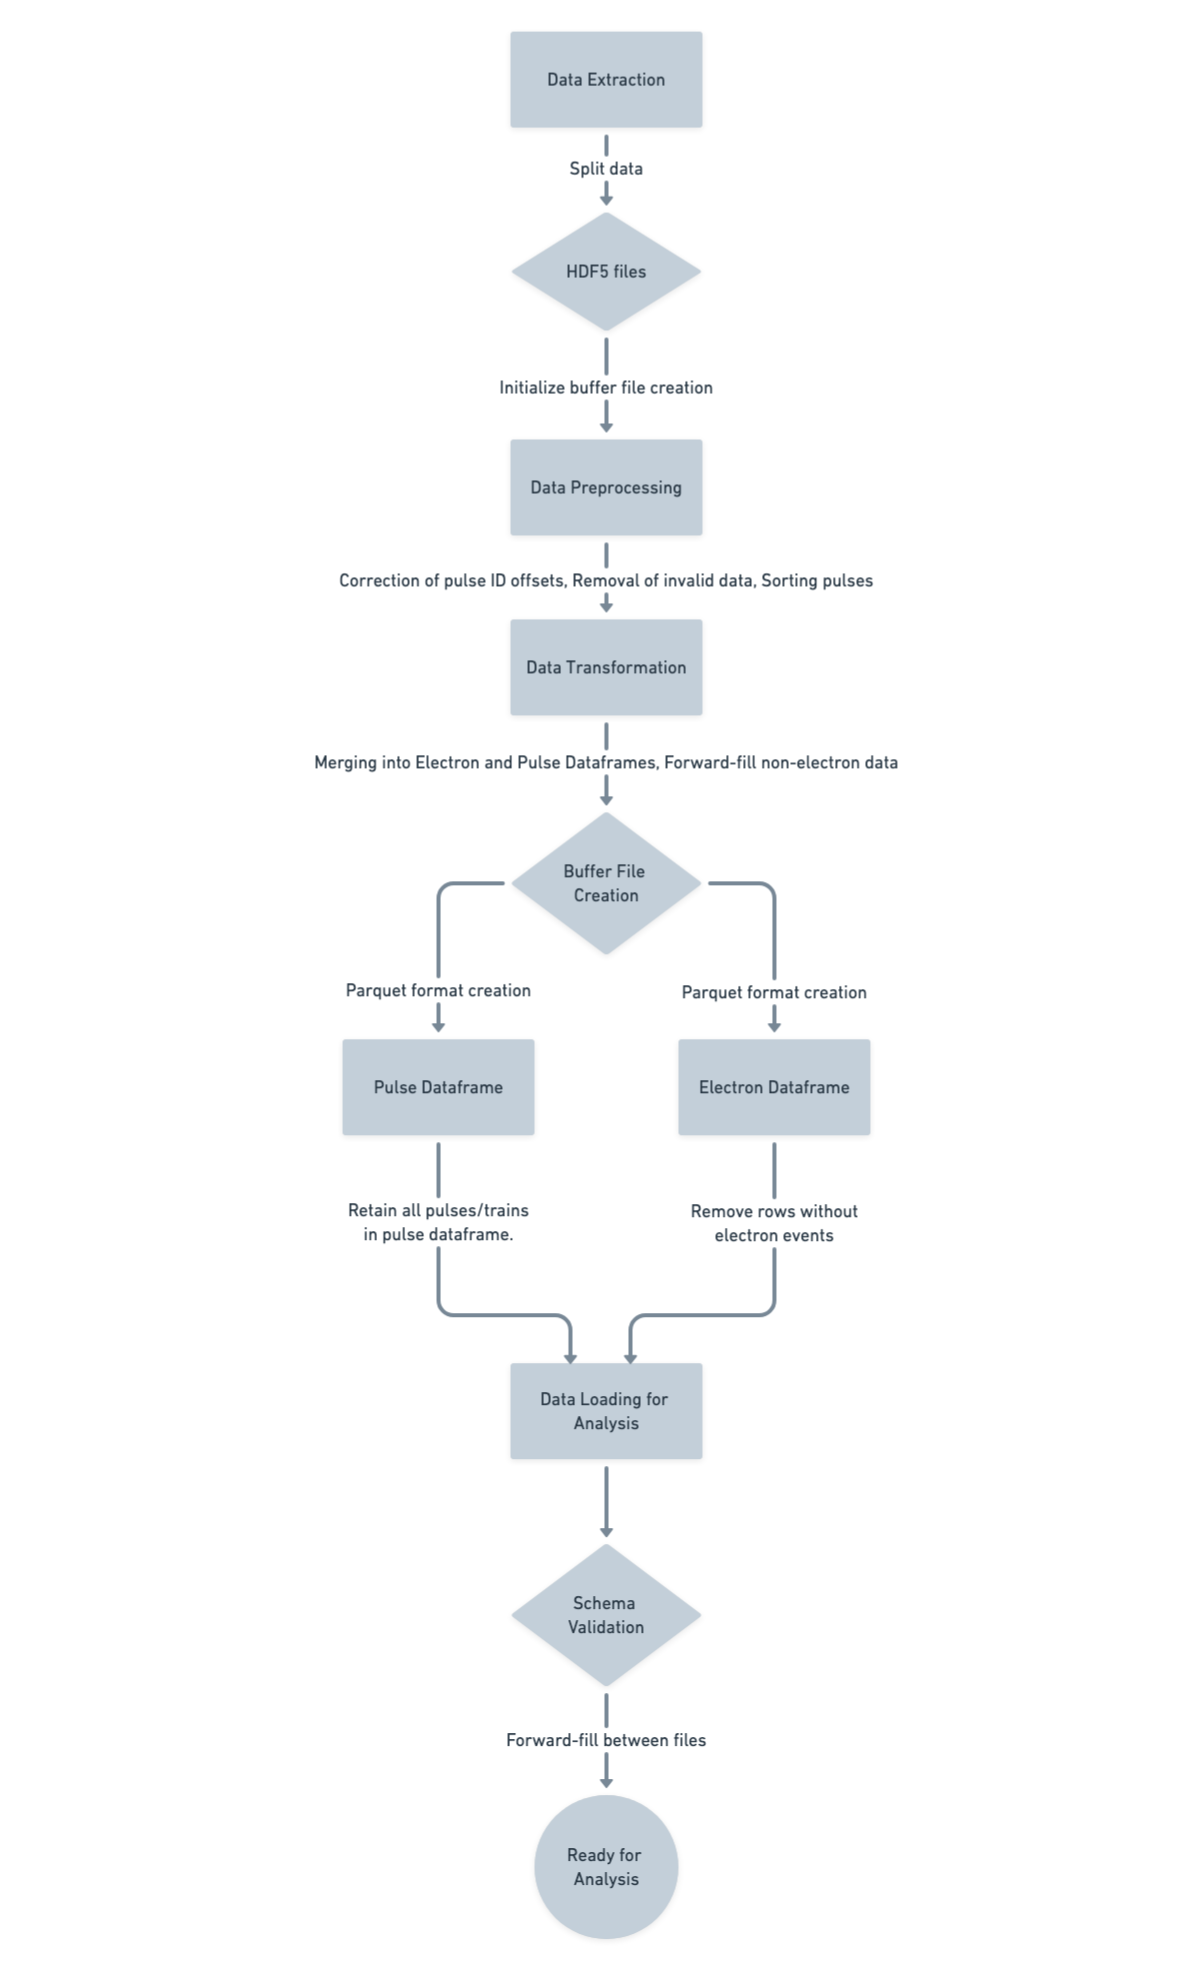
\includegraphics[width=0.7\linewidth]{images/elt_cropped.png}
    \caption{Complete \gls{ELT} pipeline for the data from \gls{HEXTOF} at \gls{FLASH}}
\end{figure}

\section{Metrics}

\Gls{MSE} is a common measure of the average squared differences between predicted values and actual values. It quantifies the error in a model’s predictions, where lower values indicate better performance. It is sensitive to outliers since squaring the differences amplifies larger errors.

\begin{note}
    {\Glsxtrfull{MSE}}
    \begin{equation}\label{eq:mse}
        \text{MSE} = \frac{1}{N} \sum_{i=1}^{N} (x_i - y_i)^2
    \end{equation}
    \begin{itemize}
        \item $x_i$: pixel value of the noisy image
        \item $y_i$: pixel value of the target image
        \item $N$: total number of pixels
    \end{itemize}
\end{note}

\Gls{PSNR} is a measure of the peak error between two images, often used to evaluate image compression quality. It expresses the ratio between the maximum possible power of a signal and the power of corrupting noise. Higher PSNR values indicate better quality.

\begin{note}
    {\Glsxtrfull{PSNR}}
    \begin{equation}    
        \text{PSNR} = 10 \log_{10} \left( \frac{L^2}{\text{MSE}} \right)
    \end{equation}
    \begin{itemize}
        \item $L$: maximum pixel value of the image
        \item \gls{MSE}: mean squared error
    \end{itemize}
\end{note}


\Gls{SSIM} is a perceptual metric that quantifies the visual impact of three characteristics of an image: luminance, contrast, and structure. It evaluates the similarity between two images based on their structural information, making it more aligned with human visual perception than MSE or PSNR. Values range from -1 to 1, with 1 indicating perfect similarity.
\begin{note}
    {\Glsxtrfull{SSIM}}
    \begin{equation}    
        \text{SSIM}(x, y) = \frac{(2\mu_x \mu_y + C_1)(2\sigma_{xy} + C_2)}{(\mu_x^2 + \mu_y^2 + C_1)(\sigma_x^2 + \sigma_y^2 + C_2)}
    \end{equation}
    \begin{itemize}
        \item $\mu_x, \mu_y$: mean of $x$ and $y$
        \item $\sigma_x, \sigma_y$: standard deviation of $x$ and $y$
        \item $\sigma_{xy}$: covariance of $x$ and $y$
        \item $C_1 = (k_1L)^2, C_2 = (k_2L)^2$: constants to stabilize the division
    \end{itemize}
\end{note}

\Gls{MSSSIM} extends \gls{SSIM} by evaluating image similarity across multiple scales and resolutions. By considering different image scales, it captures more information about structural variations and perceptual quality, making it particularly useful for assessing image quality in applications like compression. Similar to \gls{SSIM}, higher values indicate greater similarity.

\begin{note}
    {\Glsxtrfull{MSSSIM}}
    \begin{equation}    
        \text{MSSSIM}(x, y) = \prod_{j=1}^{J} \text{SSIM}(x_j, y_j)^{\alpha_j}
    \end{equation}
    \begin{itemize}
        \item $J$: number of scales
        \item $x_j, y_j$: images at scale $j$
        \item $\alpha_j$: weight for scale $j$, summing to 1
    \end{itemize}
\end{note}


\section{Experiment: Metric Comparison}\label{sec:metric_comparison_experiment}

The objective of this experiment is to evaluate the effectiveness of various image quality metrics (\gls{MSE}, \gls{PSNR}, \gls{SSIM}, and \gls{MSSSIM}) when the provided reference is noisy. Specifically, reconstructed images from a trained neural network, that has shown clear improvements in perpetual quality, are compared against the high-count but noisy reference. Examples of such images at different counts can be seen in Figure~\ref{fig:images-noisy-denoised}, which shows how the noisy images are devoid of any features at low counts, while the denoised images show clear features similar to the target. For this analysis, it is not relevant if the high quality reconstructions are due to overfitting or not, but rather that they produce perpetually better quality images (sometimes even compared to the target). So the hope is that the metrics acknowledge this improvement.

\begin{figure}[h]
    \centering
    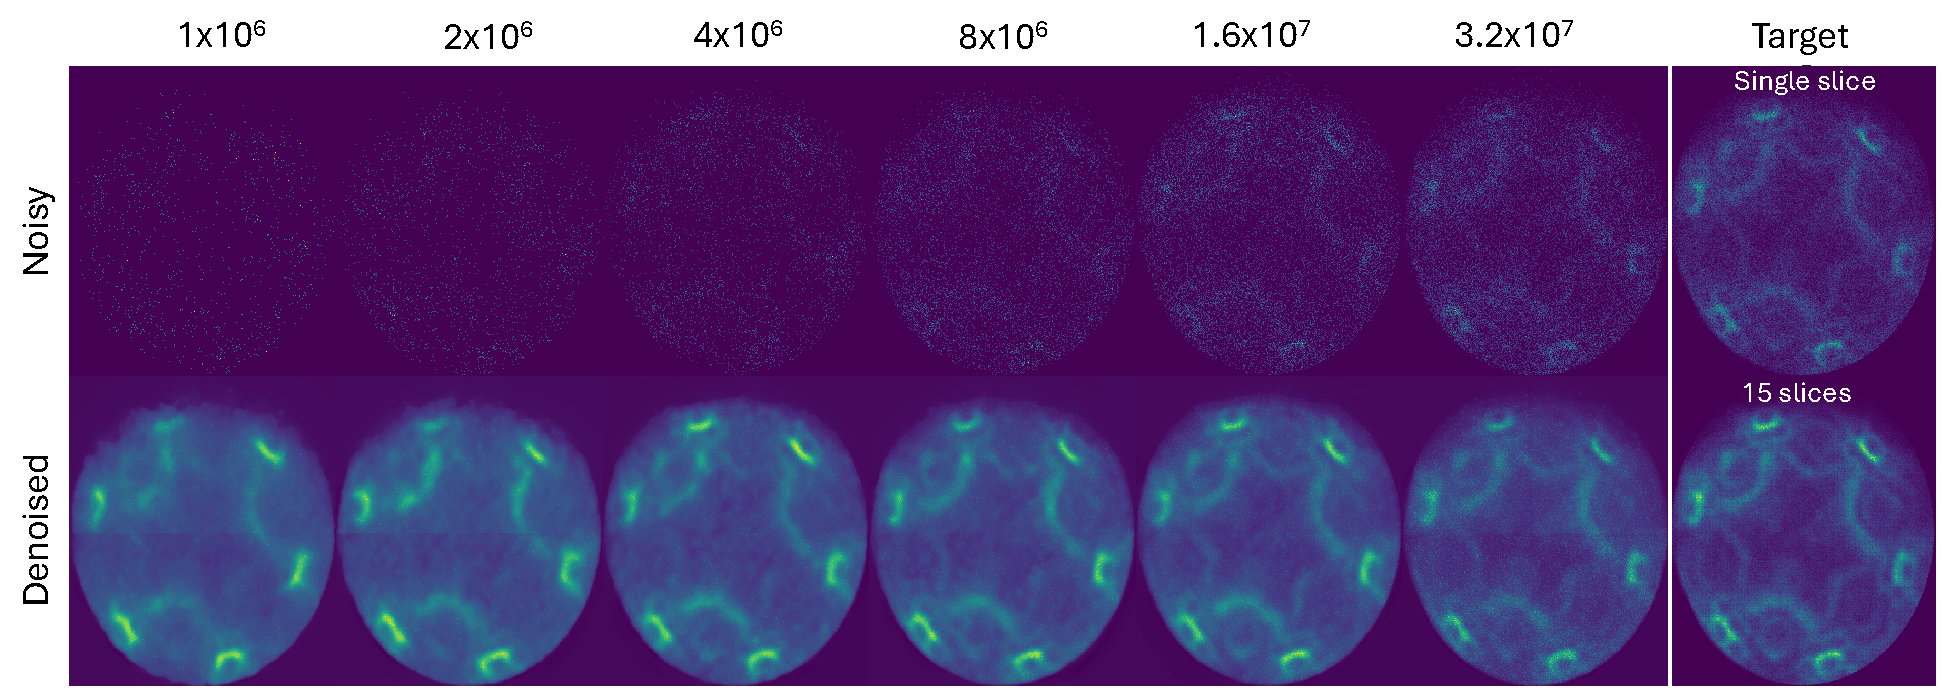
\includegraphics[width=1\linewidth]{images/images_noisy_denoised_with_target.pdf}
    \caption{Noisy and denoised \gls{ky}-\gls{kx} cuts with window size $w=1$ shown for \gls{GrIr} dataset. Each column corresponds to \numlist{1e6;2e6;4e6;8e6;1.6e7;3.2e7;1.86e8} counts, respectively; where the last column is the target image with $w=1$ in row 1 and $w=15$ in row 2. Below \num{8e6} counts, none of the features are discernible for noisy images, while the denoised images show clear features similar to the target.}
    \label{fig:images-noisy-denoised}
\end{figure}

The \gls{GrIr} dataset is used, with electron counts ranging from \numrange{1e6}{3.2e7}. For each total count, a set of 2D noisy images (referred to as noisy slices) is extracted from the dataset. Corresponding high-count 2D slices (referred to as target slices) are used as reference images for comparison (from the dataset with \num{1.86e8} counts). Likewise, reconstructed images from the neural network are also compared against the target slices.

\begin{table}[h]
    \centering
    \caption{Comparison Types and Metrics}
    \begin{tabular}{p{0.24\linewidth} | p{0.49\linewidth} | p{0.19\linewidth}}
        \hline
        \textbf{Comparison Type} & \textbf{Description} & \textbf{Metrics Evaluated} \\
        \hline
        Noisy & Input image is a noisy realization of target & MSE, PSNR, SSIM, MS-SSIM \\
        \hline
        Denoised & Input image is perpetually of better quality & MSE, PSNR, SSIM, MS-SSIM \\
        \hline
    \end{tabular}
    \caption{Comparison types and metrics evaluated in the experiment. This is repeated for single slice and window-averaged images.}
    \label{tab:comparison_types}
\end{table}

The metric evaluation procedure involves a data loader, implemented using the \texttt{PyTorch Dataset} class, which iterates through the different datasets and extracts noisy and target 2D image slices (window-averaged or single slice). For each pair of noisy and target slices, the metrics are computed. The comparison results are then grouped by acquisition count and type (noisy vs. denoised).

This metric comparison is performed with \num{1638} images sliced along each dimension of the dataset. The results are aggregated and a 95\% confidence interval is calculated for each metric to assess the reliability of the comparison. Table~\ref{tab:comparison_types} summarizes the comparison types and metrics evaluated in this experiment, repeated for both single slice and window-averaged images.


\begin{figure}[h]
    \centering
    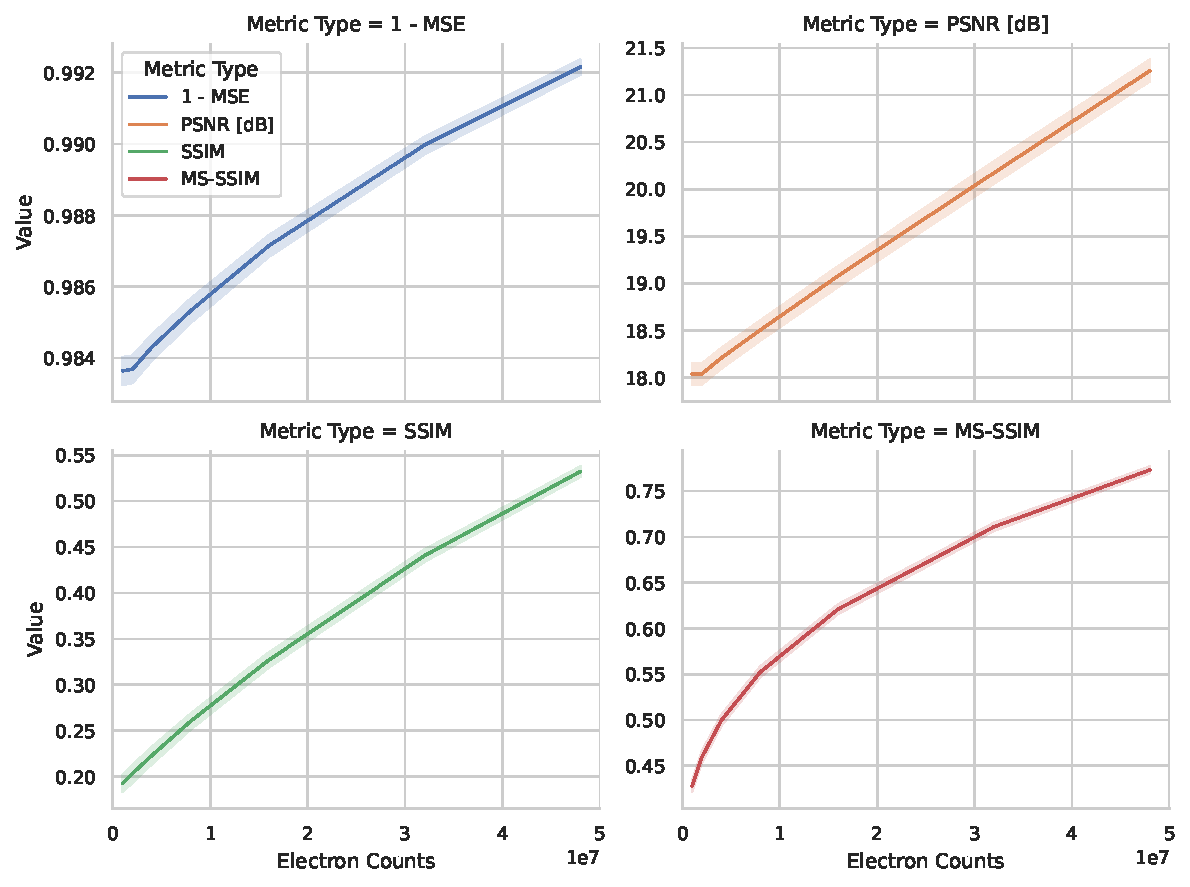
\includegraphics[width=0.7\linewidth]{images/metrics_comparison_same_target.pdf}
    \caption{Comparison of image quality metrics (\gls{MSE}, \gls{PSNR}, \gls{SSIM}, \gls{MSSSIM}) with noisy realization of a noisy target. The metrics show improved results with increased electron counts, as noise levels decrease. \gls{MSSSIM} shows the best relative improvement in metrics lower counts below \num{e7}.}
    \label{fig:metrics-comparison-noisy}
\end{figure}

Comparing the noisy images with target, all metrics trivially show an improvement with increased counts (less noise) (see Figure~\ref{fig:metrics-comparison-noisy}). However, \gls{MSE}, \gls{PSNR} and \gls{SSIM} show deteriorated metrics when comparing against perpetually high quality images (Figure~\ref{fig:metrics-comparison}). This can be attributed to the presence of noise in the reference image. For higher counts, \gls{SSIM} manages to show improved results, whereas \gls{MSE} report \gls{PSNR} consistently worse results compared to the noisy images. \gls{MSSSIM} consistently reports better results with the higher quality images, making it the most reliable metric for evaluation.

\begin{figure}
    \centering
    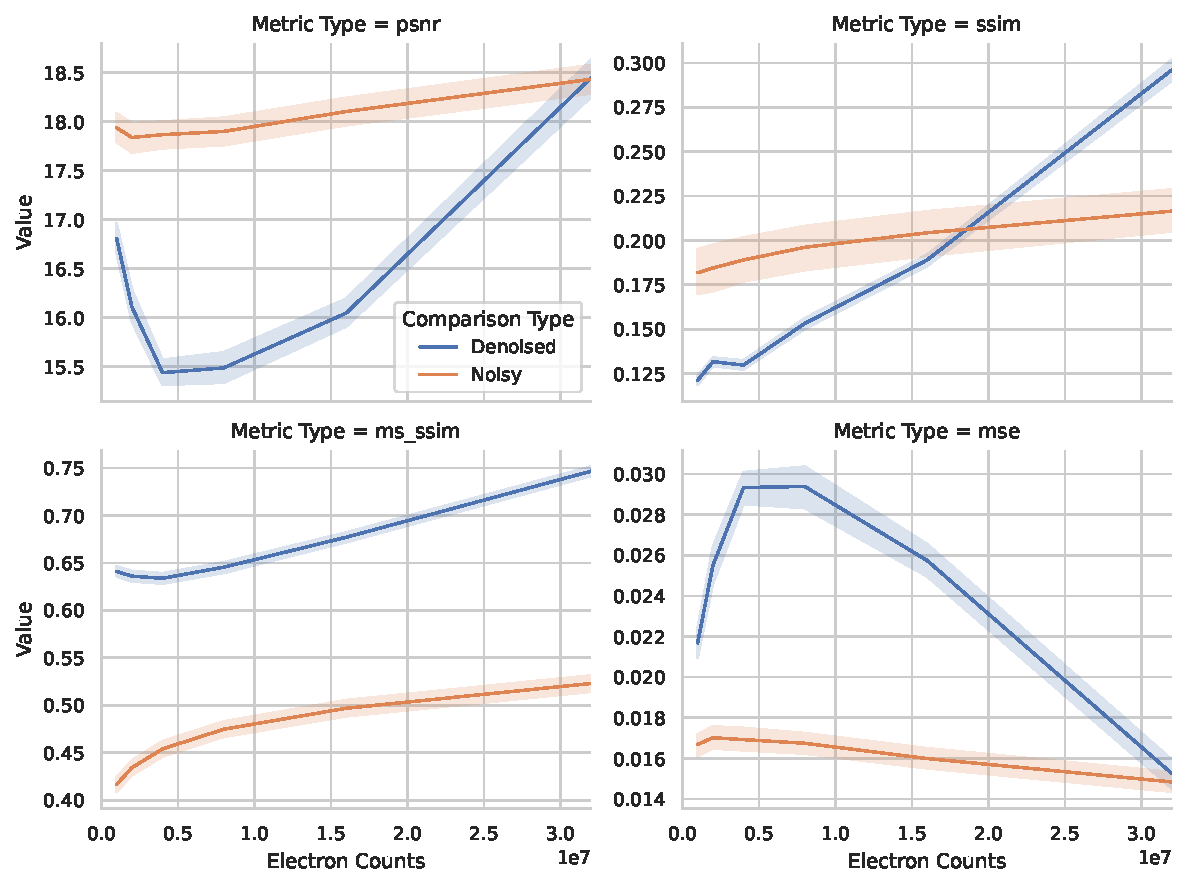
\includegraphics[width=0.7\linewidth]{images/metrics_comparison_denoised_noisy.pdf}
    \caption{Shows comparison of evaluating metrics (\gls{MSE}, \gls{PSNR}, \gls{SSIM}, \gls{MSSSIM}) with the input being a noisy realization of target or denoised version of that realization. Both are compared to a high-count target that is also noisy. Trivially, all metrics show an improvement when the counts increase. However, \gls{MSE} and \gls{PSNR} evaluate better when the input is noisy, while \gls{SSIM} and \gls{MSSSIM} show better results when the input is denoised. The gap between noisy and denoised is more pronounced for \gls{MSSSIM} than \gls{SSIM}, hence the better metric. }
   \label{fig:metrics-comparison}
\end{figure}

Additionally, we investigate the effect of window-averaged reference images on the metrics. Results indicate that window-averaged references improve metric outcomes, as the gap between the metrics calculated with noisy and high quality images split up further. Consequently, we adopt the window-averaged images as reference for the denoising evaluation.


\begin{figure}
    \centering
    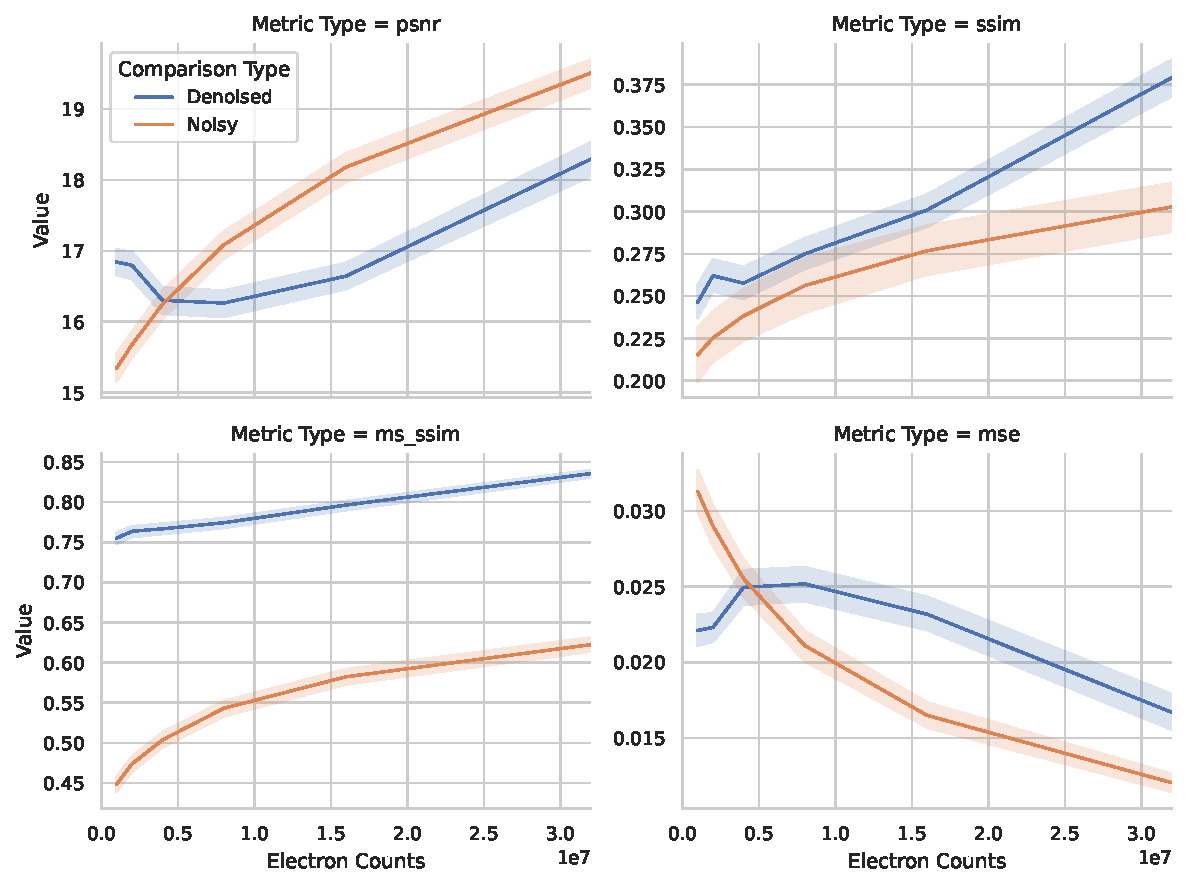
\includegraphics[width=0.7\linewidth]{images/metrics_comparison_denoised_noisy_averaged.pdf}
    \caption{Metrics comparison for noisy 2D slices against a window-averaged target slice. The window-averaged target does not significantly improve the reported metrics, showing that averaging over neighboring slices reduces resolution and does not offer a superior reference for denoising evaluation.}
    \label{fig:metrics-comparison-averaged-target}
\end{figure}


\subsection{Deep Learning Infrastructure}
Model Architecture: UNET 2D and 3D

Trained on A100 GPU 80 GB using Maxwell Cluster at DESY. 

\section{Supplementary Figures for Deep Learning based Denoising}
\begin{figure}[h]
    \centering
    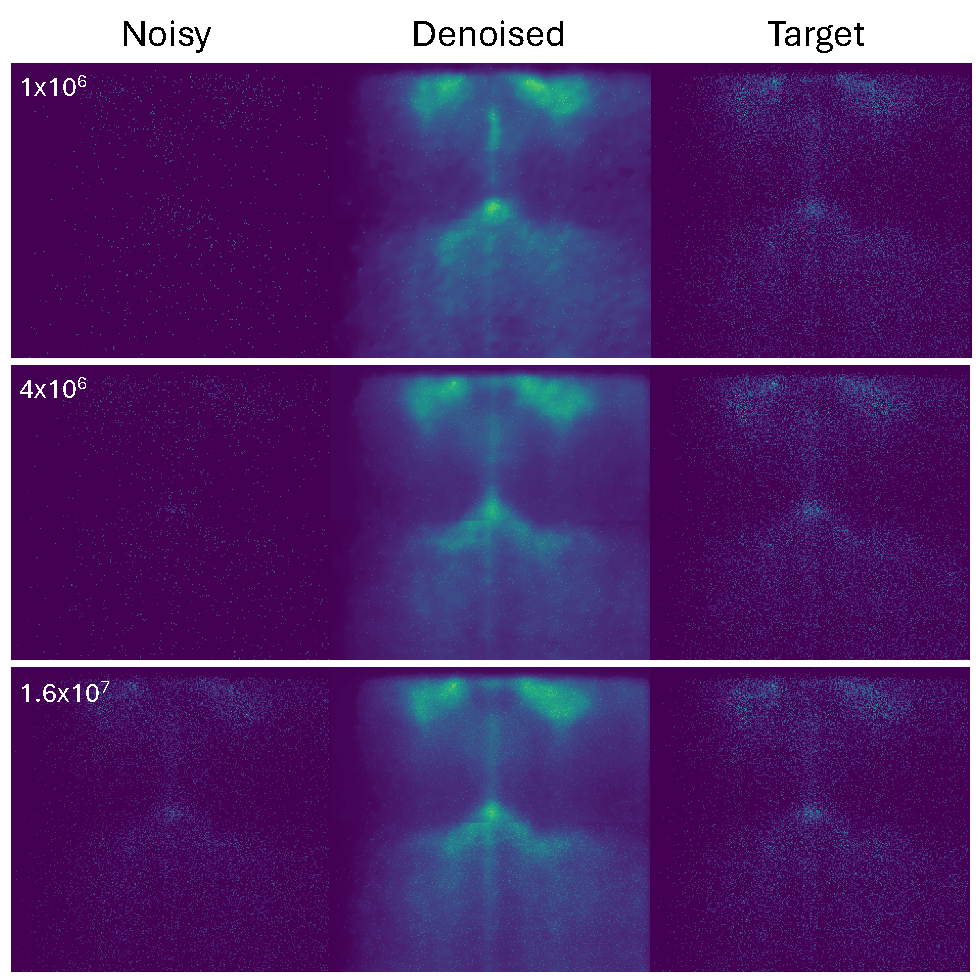
\includegraphics[width=1\linewidth]{images/nn_denoised_ex_single_slice.pdf}
    \caption{Noisy, denoised, and target \gls{E}-\gls{kx} cuts with window size $w=1$ shown for \gls{GdW} dataset. Each row corresponds \numlist{1e6;4e6;1.6e7} counts, respectively.}
    \label{fig:nn-denoised-ex-single-slice}
\end{figure}

\begin{figure}[h]
    \centering
    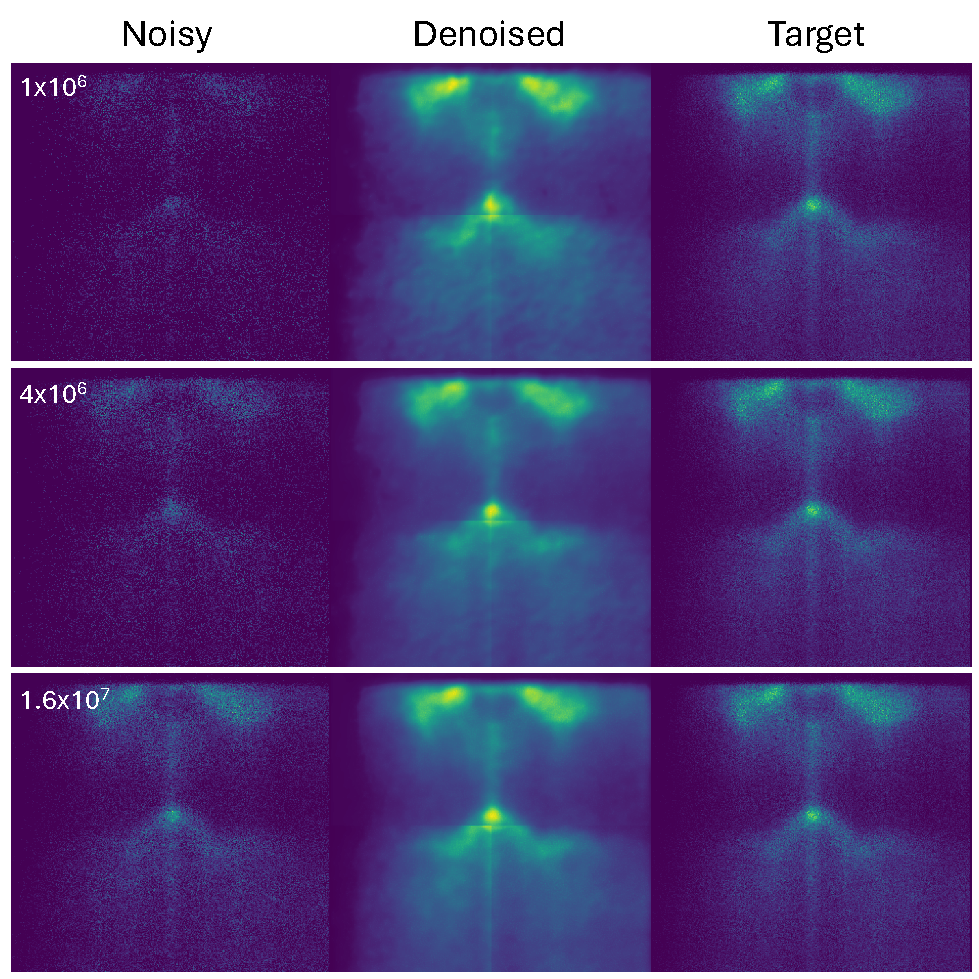
\includegraphics[width=1\linewidth]{images/nn_denoised_ex_20_slice.pdf}
    \caption{Noisy, denoised, and target \gls{E}-\gls{kx} cuts with window size $w=20$ shown for \gls{GdW} dataset. Each row corresponds \numlist{1e6;4e6;1.6e7} counts, respectively.}
    \label{fig:nn-denoised-ex-20-slice}
\end{figure}

\begin{figure}[h]
    \centering
    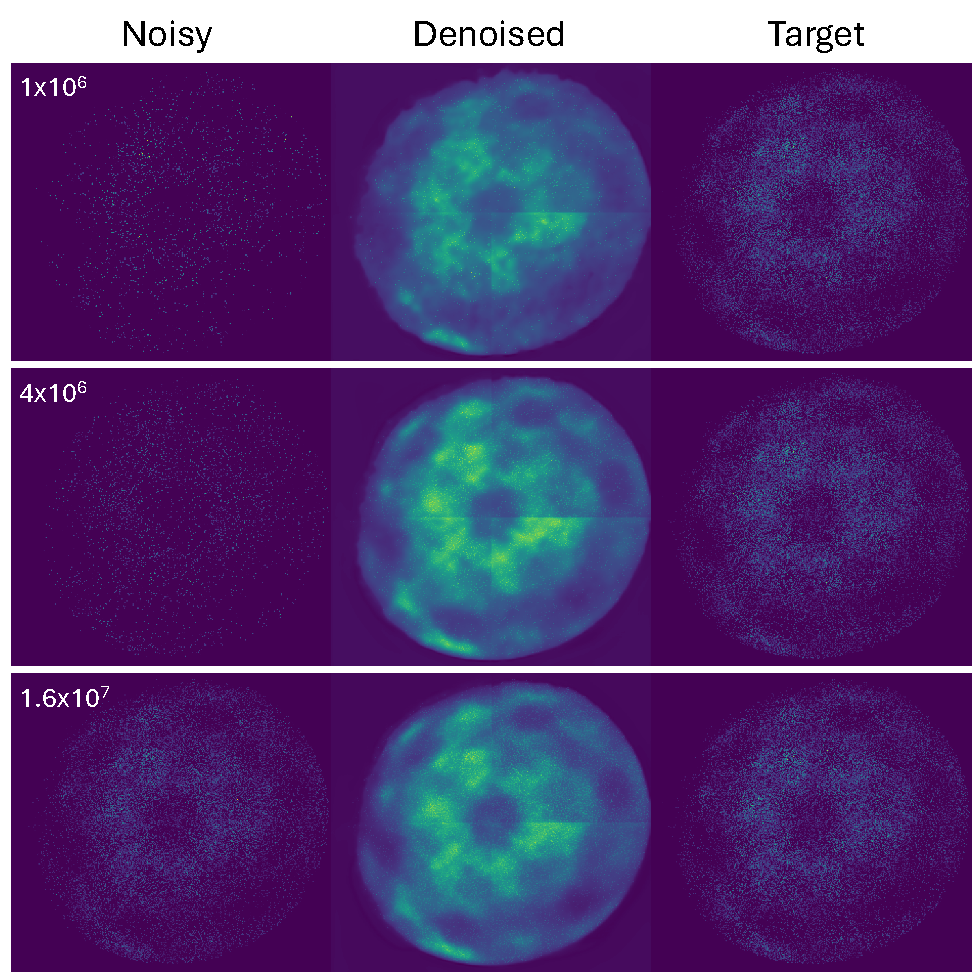
\includegraphics[width=1\linewidth]{images/nn_denoised_xy_single_slice.pdf}
    \caption{Noisy, denoised, and target \gls{ky}-\gls{kx} cuts with window size $w=1$ shown for \gls{GdW} dataset. Each row corresponds \numlist{1e6;4e6;1.6e7} counts, respectively.}
    \label{fig:nn-denoised-xy-single-slice}
\end{figure}

\begin{figure}[h]
    \centering
    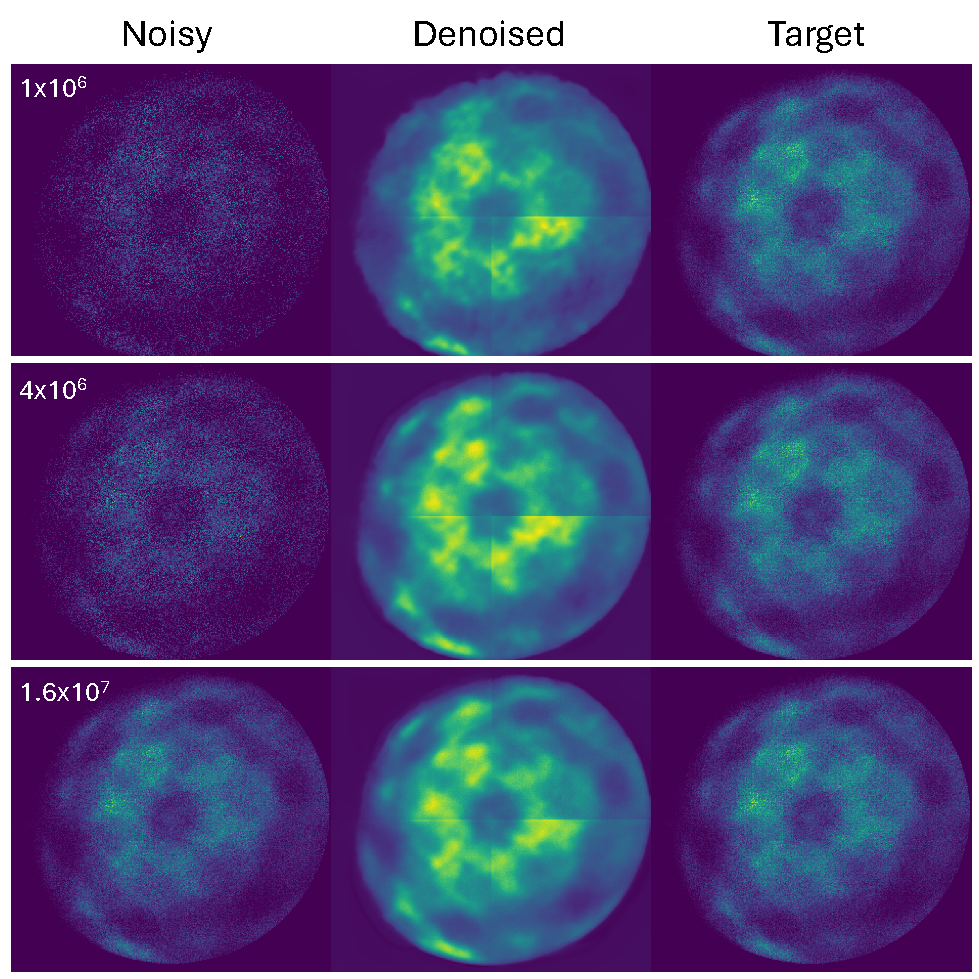
\includegraphics[width=1\linewidth]{images/nn_denoised_xy_20_slice.pdf}
    \caption{Noisy, denoised, and target \gls{ky}-\gls{kx} cuts with window size $w=20$ shown for \gls{GdW} dataset. Each row corresponds \numlist{1e6;4e6;1.6e7} counts, respectively.}
    \label{fig:nn-denoised-xy-20-slice}
\end{figure}

\break
\section{Supplementary Figures for Photoelectron Counting Statistics}
The following section outlines the counting statistics observed for \gls{PES} at two different light sources: a pulsed laser (\gls{WSe2} dataset), and a \gls{SASE} \gls{FEL} light source (\gls{GrIr} dataset). 

\cref{fig:wse2-stats-2} shows the distribution of photoelectron counts for different time intervals ($\Delta t$) within a volumetric subset of the full \gls{WSe2} dataset. The count distributions for smaller time intervals ($\Delta t = \qtylist{2;10;20}{ms}$) follow Poisson statistics, as expected from an uncorrelated photoemission process where spatial and temporal fluctuations are minimal. However, for longer time intervals ($\Delta t = \qty{50}{ms}$), the distribution starts to deviate from the Poisson distribution. This deviation suggests that spatial correlations, due to the material properties of the sample, become significant enough to impact the distribution. While the impact of pulse light source should be minimal since the time intervals we look at are much longer than the pulse durations, the spatial correlations could be due to the material properties of the sample.


The \gls{GrIr} dataset reveals more complex photoelectron count statistics over a broader range of time intervals. Figures \ref{fig:grir-stats-1}, \ref{fig:grir-stats-2}, and \ref{fig:grir-stats-3} show photoelectron count distributions for varying time windows ($\Delta t = \qtylist{10;50;100;500;1000;5000}{ms}$) in the acquisition time $T\approx\qty{30}{hour}$


\begin{figure}
    \centering
    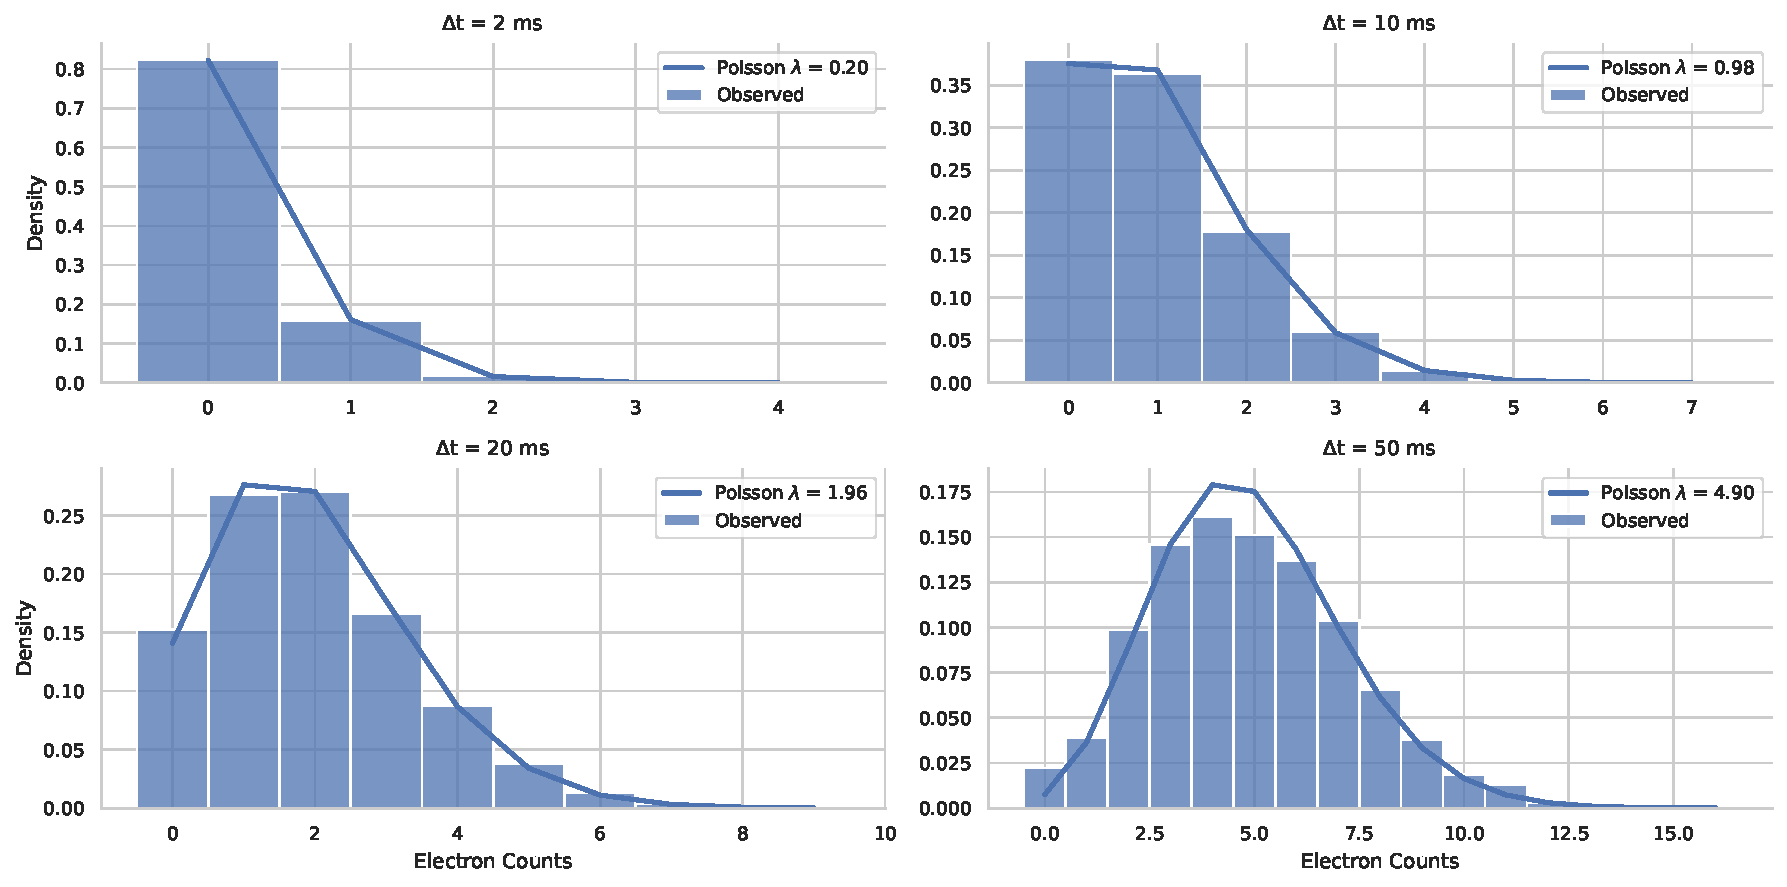
\includegraphics[width=1\linewidth]{images/hist_counts_facetgrid_2_wse2.pdf}
    \caption{Distribution of photoelectron counts at time intervals $\Delta t =$ \qtylist{2;10;20;50}{ms} for a different volumetric subset of the full \gls{WSe2} dataset. Poisson statistics are observed at smaller time intervals, but as the time window increases ($\Delta t =$ \qty{50}{ms}), the data starts to deviate from the Poisson distribution, as spatial correlations become apparent.}
    \label{fig:wse2-stats-2}
\end{figure}

\begin{figure}
    \centering
    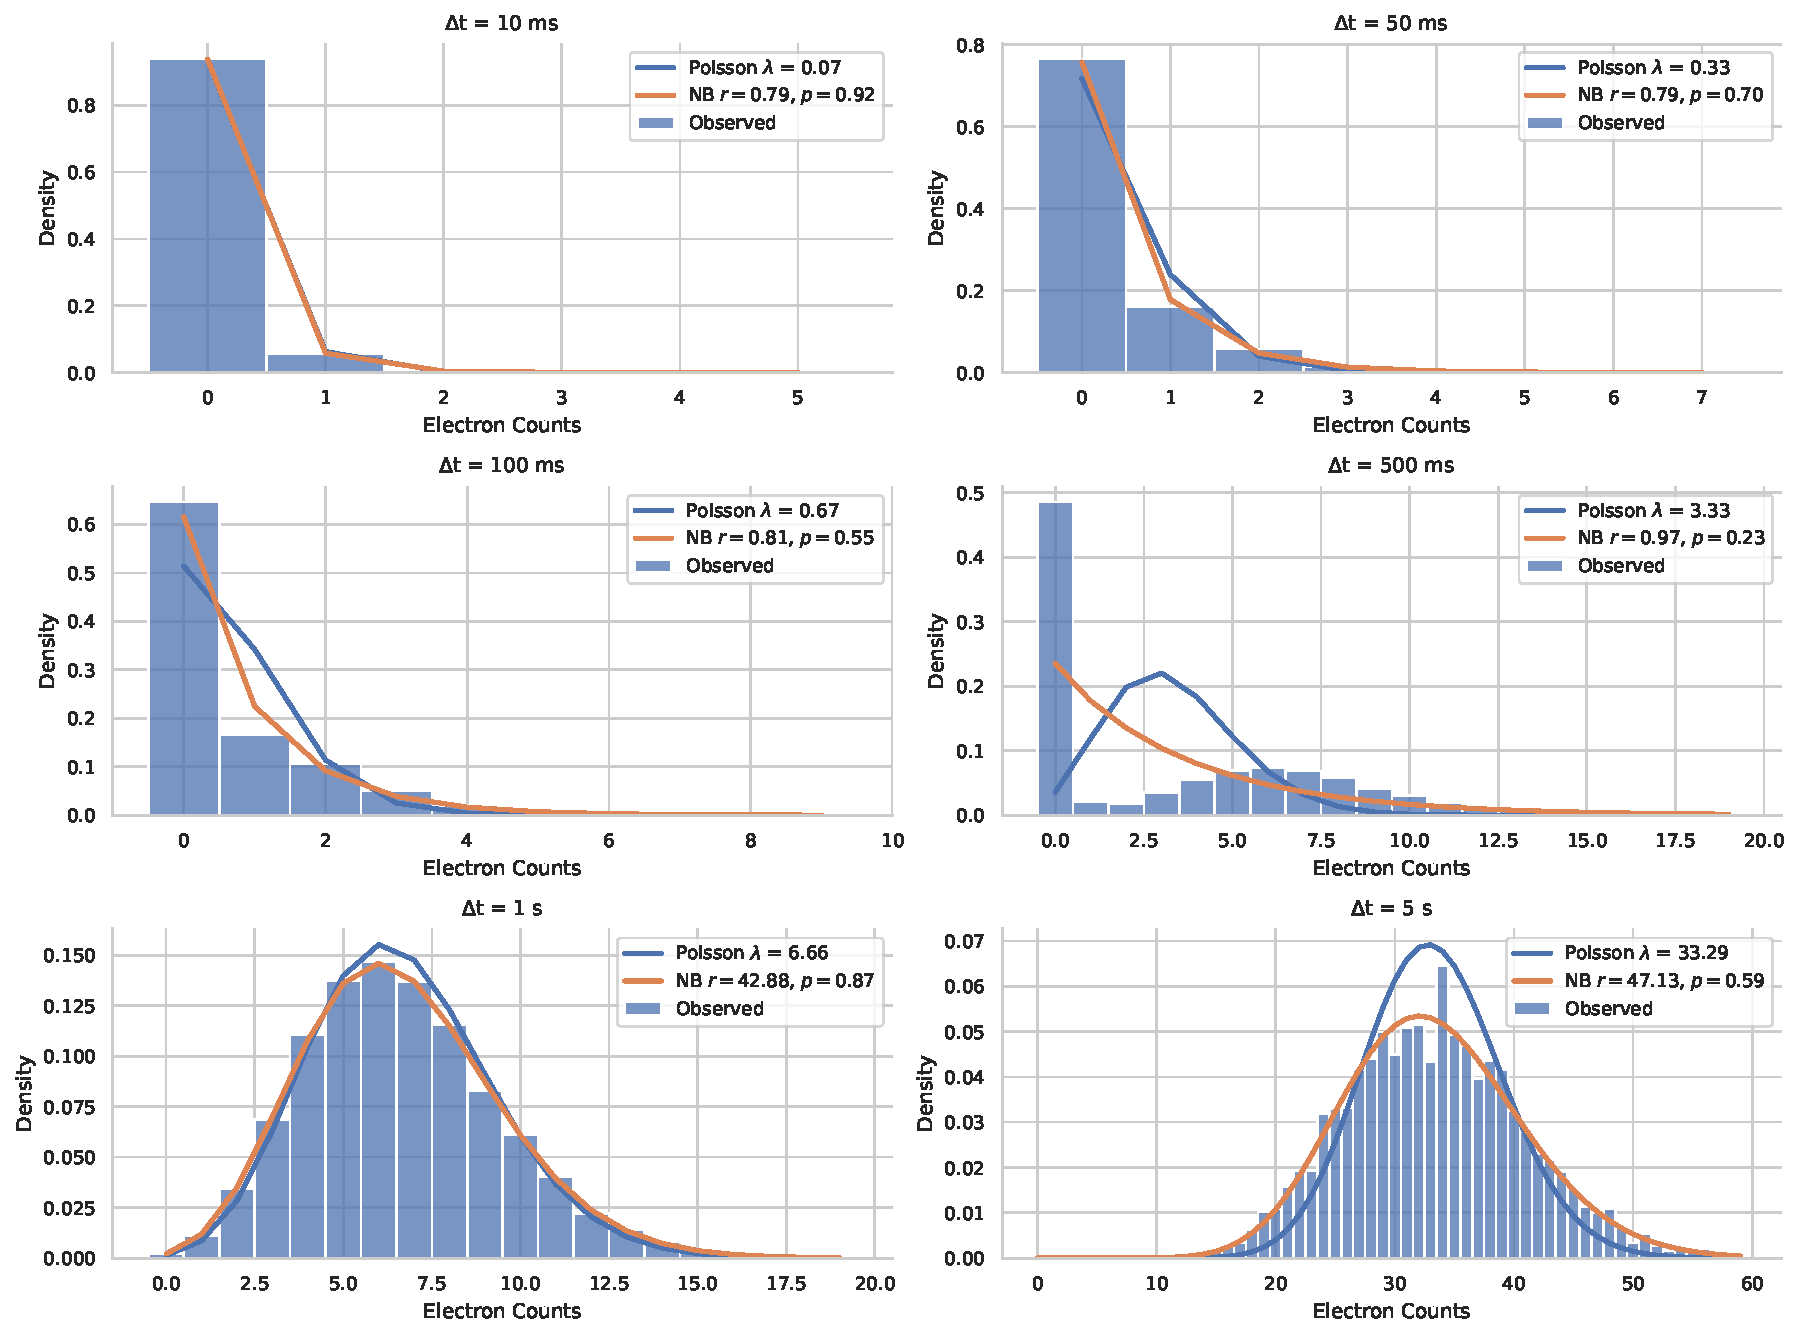
\includegraphics[width=1\linewidth]{images/hist_counts_facetgrid_3_grir.pdf}
    \caption{Distribution of photoelectron counts at time intervals $\Delta t =$ \qtylist{10;50;100;500;1000;5000}{ms} for a selected volumetric subset of the full \gls{GrIr} dataset. Poisson statistics provide a good fit at $\Delta t \leq \qty{100}{ms}$. However, for intervals $\Delta t =$ \qtylist{0.5;1;5}{s} the distribution exhibits over dispersion with a right-skewed tail, characteristic of the \gls{NB} distribution. The total counts in this selected region are $\gls{ncounts}=\num{1e6}$ with total observation time $T\approx\qty{4}{h}$  (See red region in \cref{fig:gmd-intensity}). The smaller $\Delta t$ values may represent the limiting case of the \gls{NB} distribution approaching Poisson statistics.}
    \label{fig:grir-stats-3}
\end{figure}
% \subsection{Mathematical Formulation}
% As shown in \cref{alg:bm3d} and \cref{fig:bm3d-schematic}, the \gls{BM3D} scheme is a two-stage image denoising algorithm that exploits non-local image similarities. The algorithm processes a noisy image $X$ to produce a denoised estimate $\hat{Y}$ through collaborative filtering of similar patches.

% Stage 1: Basic Estimate

% The first stage produces a basic estimate through the following steps:

% 1. **Block Matching**: For each reference block $B_r$ of size $N_1 \times N_1$ in the noisy image, similar blocks are found using the normalized $l^2$-distance:
   
%    $$d(B_r, B_k) = \frac{\|B_r - B_k\|_2^2}{N_1^2}$$

%    Blocks with distance below a threshold $\tau_{\text{match}}$ are grouped:
   
%    $$\mathcal{S}(B_r) = \{B_k : d(B_r, B_k) \leq \tau_{\text{match}}\}$$

% 2. **3D Block Formation**: Similar blocks are stacked into a 3D array $\mathcal{Z}$ of size $N_1 \times N_1 \times |\mathcal{S}(B_r)|$:
   
%    $$\mathcal{Z} = [B_r | B_{k_1} | B_{k_2} | ... | B_{k_n}]$$

% 3. **3D Transform**: A separable 3D transform $\mathcal{T}_{3D}$ is applied:
   
%    $$\mathcal{T}_{3D} = \mathcal{T}_{2D} \otimes \mathcal{T}_{1D}$$
   
%    where $\mathcal{T}_{2D}$ is typically a 2D DCT applied to each block, and $\mathcal{T}_{1D}$ is a 1D Haar transform along the similarity dimension.

% 4. **Hard Thresholding**: The transform coefficients are hard-thresholded:
   
%    $$\Gamma_{\lambda_{\text{3D}}}(\mathcal{T}_{3D}\mathcal{Z}) = 
%    \begin{cases} 
%    (\mathcal{T}_{3D}\mathcal{Z})_{i,j,k} & \text{if } |(\mathcal{T}_{3D}\mathcal{Z})_{i,j,k}| > \lambda_{\text{3D}} \\
%    0 & \text{otherwise}
%    \end{cases}$$

% 5. **Inverse Transform and Aggregation**: The filtered blocks are transformed back and aggregated with weights $w_{B_r}$ based on the number of non-zero coefficients after thresholding:
   
%    $$\hat{Y}_{\text{basic}} = \frac{\sum_{B_r} w_{B_r} \cdot \mathcal{T}_{3D}^{-1}(\Gamma_{\lambda_{\text{3D}}}(\mathcal{T}_{3D}\mathcal{Z}))}{\sum_{B_r} w_{B_r}}$$

% Stage 2: Final Estimate

% The second stage uses the basic estimate to perform Wiener filtering:

% 1. **Block Matching**: In the second stage, the block matching uses both the noisy image $X$ and the basic estimate $\hat{Y}_{\text{basic}}$. The distance between blocks is computed as:
% $$d_2(B_r, B_k) = |B_r^{\text{basic}} - B_k^{\text{basic}}|2^2 = \sum{i,j} (B_r^{\text{basic}}[i,j] - B_k^{\text{basic}}[i,j])^2$$
% where $B_r^{\text{basic}}$ and $B_k^{\text{basic}}$ are blocks from the basic estimate $\hat{Y}_{\text{basic}}$. The grouping in the second stage creates a set:
% $$B = {B_k : d_2(B_r, B_k) \leq \tau_2}$$
% where $\tau_2$ is the threshold for the second stage. The corresponding blocks from the noisy image $X$ are then used for the actual Wiener filtering, but their grouping is determined by the similarity of blocks in the basic estimate.
% This approach is more reliable than using the noisy image alone because the basic estimate has reduced noise, leading to more accurate block matching.

% 2. **Wiener Filtering**: For each 3D group $\mathcal{Z}$, the Wiener shrinkage coefficients are:

%    $$W_{i,j,k} = \frac{|(\mathcal{T}_{3D}\mathcal{Z}_{\text{basic}})_{i,j,k}|^2}{|(\mathcal{T}_{3D}\mathcal{Z}_{\text{basic}})_{i,j,k}|^2 + \sigma^2}$$

%    where $\mathcal{Z}_{\text{basic}}$ is the corresponding group from $\hat{Y}_{\text{basic}}$ and $\sigma^2$ is the noise variance.

% 3. **Final Estimate**: The final estimate is obtained by:

%    $$\hat{Y} = \frac{\sum_{B_r} w_{B_r} \cdot \mathcal{T}_{3D}^{-1}(W \cdot \mathcal{T}_{3D}\mathcal{Z})}{\sum_{B_r} w_{B_r}}$$

% This two-stage approach is particularly effective because the Wiener filter coefficients are computed using the basic estimate, which provides a more reliable power spectrum estimate than the noisy image alone.
% \begin{algorithm}
%     \caption{BM3D Denoising Algorithm}\label{alg:bm3d}
%     \begin{algorithmic}[1]
%     \Require Noisy image $X$, noise variance $\sigma^2$
%     \Ensure Denoised image $\hat{Y}$
%     \Statex
%     \State // Stage 1: Basic Estimate
%     \State $\hat{Y}_{\text{basic}} \gets \textsc{BasicEstimate}(X, \sigma^2)$
%     \State // Stage 2: Final Estimate
%     \State $\hat{Y} \gets \textsc{WienerFiltering}(X, \hat{Y}_{\text{basic}}, \sigma^2)$
%     \State \textbf{return} $\hat{Y}$
%     \end{algorithmic}
% \end{algorithm}

% \begin{algorithm}
%     \caption{Basic Estimate}\label{alg:basicestimate}
%     \begin{algorithmic}[1]
%     \Require Noisy image $X$, noise variance $\sigma^2$
%     \Ensure Basic estimate $\hat{Y}_{\text{basic}}$
%     \For{each reference block $B_r$ in $X$}
%         \State $\mathcal{S}(B_r) \gets \{B_k : d(B_r, B_k) \leq \tau_{\text{match}}\}$ \Comment{Block matching}
%         \State $\mathcal{Z} \gets \text{Stack}(B_r, \mathcal{S}(B_r))$ \Comment{3D array formation}
%         \State $\mathcal{T}_{3D}\mathcal{Z} \gets \textsc{3DTransform}(\mathcal{Z})$
%         \State $\mathcal{Z}_{\text{filtered}} \gets \Gamma_{\lambda_{\text{3D}}}(\mathcal{T}_{3D}\mathcal{Z})$ \Comment{Hard thresholding}
%         \State $\mathcal{Z}_{\text{spatial}} \gets \textsc{3DInverseTransform}(\mathcal{Z}_{\text{filtered}})$
%         \State Update $\hat{Y}_{\text{basic}}$ with weighted $\mathcal{Z}_{\text{spatial}}$
%     \EndFor
%     \State \textbf{return} $\hat{Y}_{\text{basic}}$
%     \end{algorithmic}
% \end{algorithm}
  % \input{jupyter_notebooks/notebooks.tex}
\end{appendices}

\end{document}
